\documentclass{article}

\usepackage{amsmath}
\usepackage{amsfonts}
\usepackage{amssymb}
\usepackage{multicol}
\usepackage{wrapfig}
\usepackage{mathenv}
\usepackage{multirow}
\usepackage{pdfpages}
\usepackage{vmargin}
\setmarginsrb{2.5cm}{2.5cm}{2.5cm}{2.9cm}{0cm}{0cm}{0cm}{0cm}

\usepackage[utf8]{inputenc}

\usepackage[french]{babel}
\selectlanguage{french}

\usepackage{color}
\usepackage{hyperref}
\hypersetup{pdfborder={0 0 0}, colorlinks=true, urlcolor=blue, linkcolor = darkred}
\usepackage{graphicx}
\graphicspath{{pdf/}}
\usepackage{listings}
\definecolor{colKeys}{rgb}{0.75,0,0}
\definecolor{colIdentifier}{rgb}{0,0,0}
\definecolor{colComments}{rgb}{0.75,0.75,0}
\definecolor{colString}{rgb}{0,0,0.7}

\usepackage{verbatim}
\usepackage{moreverb}
\usepackage{algorithmic,algorithm}

\lstset{
basicstyle=\ttfamily\small, %
identifierstyle=\color{colIdentifier}, %
keywordstyle=\color{colKeys}, %
stringstyle=\color{colString}, %
commentstyle=\color{colComments}, %
showspaces=false,
}
\lstset{language=java}

% Commandes personnelles %

\definecolor{darkred}{rgb}{0.85,0,0}
\definecolor{darkblue}{rgb}{0,0,0.7}
\definecolor{darkgreen}{rgb}{0,0.6,0}
\definecolor{darko}{rgb}{0.93,0.43,0}
\definecolor{maintitle}{rgb}{0.66,0,0.22}
\definecolor{title}{rgb}{0,0.5,0.5}
\definecolor{quote}{rgb}{0.7,0.7,0.7}
\definecolor{forestgreen}{rgb}{0.14,0.54,0.13}
\definecolor{cyan4}{rgb}{0,0.54,0.54}
\definecolor{firebrick4}{rgb}{0.54,0.1,0.1}
\newcommand{\maintitlecolor}[1]{\textcolor{maintitle}{#1}}
\newcommand{\titre}[1]{\textcolor{title}{#1}}
\newcommand{\tsect}[1]{\titre{\section{#1}}}
\newcommand{\tssect}[1]{\titre{\subsection{#1}}}
\newcommand{\tsssect}[1]{\titre{\subsubsection{#1}}}
\newcommand{\vect}[1]{\overrightarrow{#1}}
\newcommand{\dred}[1]{\textcolor{darkred}{\textbf{#1}}}
\newcommand{\dgre}[1]{\textcolor{darkgreen}{\textbf{#1}}}
\newcommand{\dblu}[1]{\textcolor{darkblue}{\textbf{#1}}}
\newcommand{\dora}[1]{\textcolor{darko}{\textbf{#1}}}
\newcommand{\gre}[1]{\textcolor{darkgreen}{#1}}
\newcommand{\blu}[1]{\textcolor{darkblue}{#1}}
\newcommand{\ora}[1]{\textcolor{darko}{#1}}
\newcommand{\rouge}[1]{\textcolor{darkred}{#1}}
\newcommand{\quotecolor}[1]{\textcolor{quote}{#1}}
\newcommand{\forest}[1]{\textcolor{forestgreen}{#1}}
\newcommand{\cyan}[1]{\textcolor{cyan4}{#1}}
\newcommand{\firebrick}[1]{\textcolor{firebrick4}{#1}}
\newcommand{\ceil}[1]{\left\lceil #1 \right\rceil}
\newcommand{\cdil}[1]{\left\lfloor #1 \right\rfloor}
\newcommand{\term}[1]{\textit{\textcolor{maintitle}{#1}}}
\newcommand{\image}[1]{\includegraphics{#1}}
\newcommand{\imageR}[2]{\includegraphics[width=#2px]{#1}}
\newcommand{\imageRT}[2]{\includegraphics[height=#2px]{#1}}
\newcommand{\img}[1]{\begin{center}\includegraphics[width=400px]{#1}\end{center}}
\newcommand{\imag}[1]{\begin{center}\includegraphics{#1}\end{center}}
\newcommand{\imgR}[2]{\begin{center}\includegraphics[width=#2px]{#1}\end{center}}
\newcommand{\imgRT}[2]{\begin{center}\includegraphics[height=#2px]{#1}\end{center}}
\newcommand{\point}[2]{\item \ora{\underline{#1}} : \textit{#2}}
\newcommand{\bfp}[2]{\item \textbf{#1} : \textit{#2}}
\newcommand{\sumparam}[3]{\sideset{}{_{#1}^{#2}}\sum{#3}}
\newcommand{\sumin}[3]{\sideset{}{_{i=#1}^{#2}}\sum{#3}}
\newcommand{\sumkn}[3]{\sideset{}{_{k=#1}^{#2}}\sum{#3}}
\newcommand{\intin}[3]{\sideset{}{_{#1}^{#2}}\int{#3}}
\newcommand{\stitre}[1]{\noindent\textbf{\underline{#1}} \\}
\newcommand{\R}{\mathbb{R}}
\newcommand{\Z}{\mathbb{Z}}
\newcommand{\N}{\mathbb{N}}
\newcommand{\ualpha}{\vect{u_\alpha}}
\newcommand{\valpha}{\vect{v_\alpha}}
\newcommand{\palpha}{\vect{\Psi_\alpha}}
\newcommand{\npcomp}{\term{$\mathcal{NP}$-complet}}
\newcommand{\npcompl}{\term{$\mathcal{NP}$-complet} }
\newcommand{\cqfd}{\begin{flushright}$\square$\end{flushright}}
\newcommand{\contrad}{\begin{flushright}$\boxtimes$\end{flushright}}
\DeclareMathAlphabet{\mathpzc}{OT1}{pzc}{m}{it}
\newtheorem{de}{D\'efinition}[section]
\newtheorem{note}{Note}[section]
\newtheorem{propriete}{Propri\'et\'e}[section]
\newtheorem{exemple}{Exemple}[section]
\newtheorem{corollaire}{Corollaire}[section]
\newtheorem{interlude}{Interlude}[section]
\newtheorem{rappel}{Rappel}[section]
\newtheorem{rem}{Remarque}[section]
\newtheorem{rems}{Remarques}[section]
\newtheorem{thm}{Th\'eor\`eme}[section]
\newtheorem{lemme}{Lemme}[section]
\newtheorem{illustration}{Illustration}[section]
\newtheorem{pbm}{Problème}[section]
\newtheorem{proof}{Preuve}[section]
\renewcommand{\theproof}{\empty{}}
\newenvironment{pblm}{\hbox{\raisebox{0.4em}{\vrule depth 1pt height 0.4pt width 5cm}}\begin{pbm}}
{\end{pbm}\hbox{\raisebox{0.4em}{\vrule depth 1pt height 0.4pt width 5cm}}}

%% ALGORITHME

\floatname{algorithm}{Algorithme}
\renewcommand{\algorithmicrequire}{\textbf{Entrée :}}
\renewcommand{\algorithmicensure}{\textbf{Sortie :}}
\renewcommand{\algorithmicif}{\textbf{Si}}
\renewcommand{\algorithmicthen}{\textbf{alors}}
\renewcommand{\algorithmicelse}{\textbf{Sinon}}
\renewcommand{\algorithmicwhile}{\textbf{Tant que}}
\renewcommand{\algorithmicdo}{\textbf{faire}}
\renewcommand{\algorithmicend}{\textbf{fin}}
\renewcommand{\algorithmicreturn}{\textbf{Retourner}}
\renewcommand{\algorithmicfor}{\textbf{Pour}}

%%%%%%%%%%%%%%%%%%%%%%%%%%%%%%%%%%%%%%%%%%%%%%%%%%%%%%%%%%%%%%%%%%%
%%%%%%%%%%%%%%%%%%%%%%%% DEBUT DU DOCUMENT %%%%%%%%%%%%%%%%%%%%%%%%
%%%%%%%%%%%%%%%%%%%%%%%%%%%%%%%%%%%%%%%%%%%%%%%%%%%%%%%%%%%%%%%%%%%

\begin{sffamily}
\title{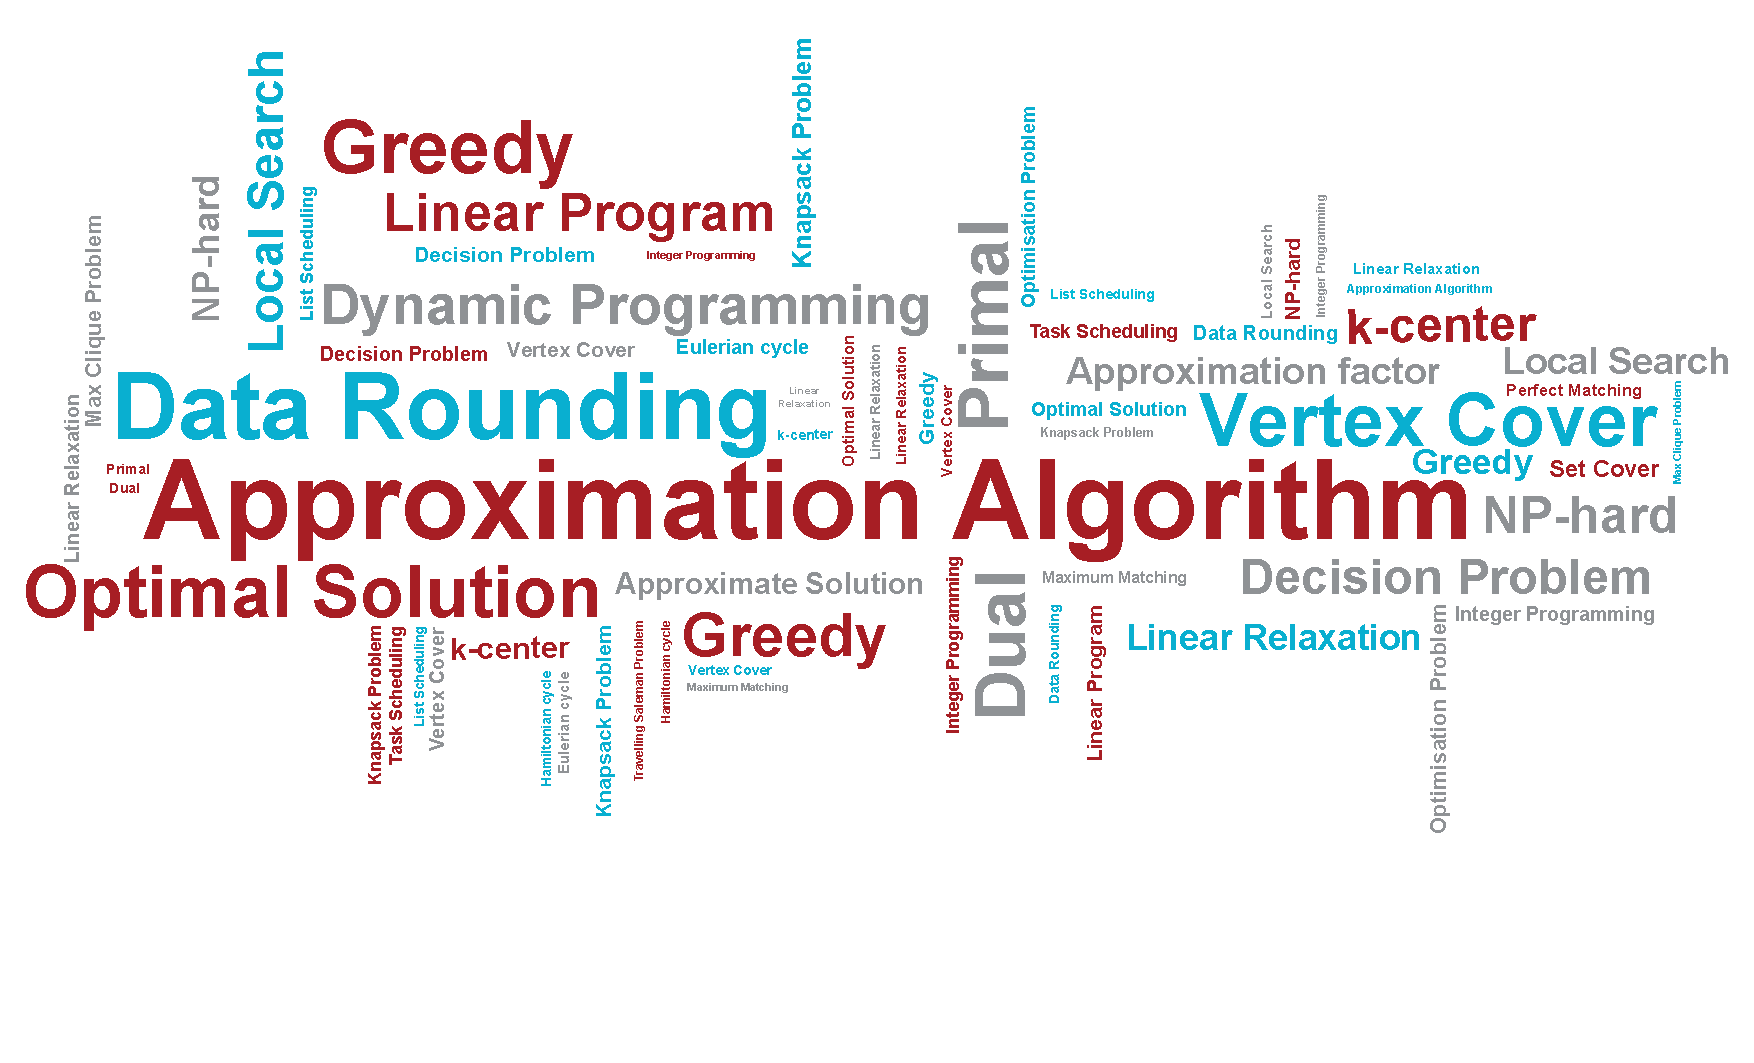
\includegraphics[scale=0.48]{approx.pdf} $ $\\
\hbox{\raisebox{0.4em}{\vrule depth 2pt height 0.4pt width \textwidth}} $ $ \\ $ $ \\
\begin{Huge}\maintitlecolor{Algorithmes d'approximation}\end{Huge} \\
$ $ \\
\begin{LARGE}\textit{Cours}\end{LARGE}}
\author{\textit{Xavier Dubuc} \\(\url{xavier.dubuc@umons.ac.be}) \\$ $ \\$ $\\$ $\\
\hbox{\raisebox{0.4em}{\vrule depth 1pt height 0.4pt width 5cm}} \\ $ $\\$ $ \\$ $\\

\includegraphics[scale=0.3]{UMONS.pdf}$\qquad \qquad$

\includegraphics[scale=0.1]{faculte.pdf}}
%\date{}
\end{sffamily}

\begin{document}\begin{sffamily}

\maketitle

\newpage

\textbf{Contributeurs:}
\renewcommand{\labelitemi}{$\bullet$}

\begin{itemize}
	\item 2016
	\begin{itemize}
		\item Benoit Debled
		\item Julien Delplanque (\url{julien.delplanque@student.umons.ac.be})
		\item Anthony Rouneau
	\end{itemize}
	\item 2017
	\begin{itemize}
		\item Florent Delgrange
	\end{itemize}
\end{itemize}

\newpage

\hbox{\raisebox{0.4em}{\vrule depth 1.5pt height 0.4pt width 10cm}}

\tableofcontents

$ $\\ \hbox{\raisebox{0.4em}{\vrule depth 1.5pt height 0.4pt width 10cm}}

\newpage

\section{Introduction}

\subsection*{Introduction au cours}

\begin{itemize}
	\item Examen oral $\rightarrow$ tirer une question et préparation de la question avec les notes, puis on présente.
	\item Travail personnel après Pâques (présentation).
\end{itemize}

\subsection*{Références}

\begin{itemize}
	\item \textbf{Williamson} \& \textbf{Shmoys} \\
	``\textit{The Design of Approximation Algorithms}''\\
	Cambridge University (version gratuite pdf  : \url{www.designofapproxalgs.com})
	\item \textbf{Vazirani}\\
	``\textit{Approximation Algorithms}''\\
	Springer, 2001 \textit{(difficile à comprendre)}
	\item \textbf{Ausiello}, \textbf{Cescenzi}, \textbf{Gambozi}, \textbf{Kann}, et al.\\
	``\textit{Complexity and Approximation : Combinatorial Optimization Problems  \\\indent \hspace{4.9cm} and their
	approximability properties}''\\
	Springer, 1999.
\end{itemize}

\subsection{Introduction à la matière}

On va voir les problèmes d'optimisation, en particulier les problèmes
\textit{NP-difficiles} ($\sim$\textit{NP-complets}, on verra  les différences
plus tard). A moins que $P = NP$, on ne peut résoudre ces problèmes
d'optimisation de manière optimale, c'est-à-dire qu'il n'existe pas (encore ?)
d'algorithme \textit{efficace} (càd polynomial) pour trouver une solution
optimale à ces problèmes. \\

\textbf{Que peut-on faire dans ces cas là ?}\textit{ (un des objectifs du cours)} \\

\noindent La première réponse est ``\textit{les heuristiques}''. Elles sont
\gre{rapides} mais elles donnent une solution qui est une \textit{``bonne"}
solution et pas \textbf{\underline{la solution optimale}} (en temps
polynomial).\\ Dans ce cours on va prouver que l'heuristique donne une solution
qui est proche de la solution optimale. \\

\noindent On utilise une analogie à la phrase bien connue :
\begin{quote}\begin{center}
\textit{\quotecolor{{\Huge ``}}
Rapide. Bon marché. Fiable. Choisissez-en deux
\quotecolor{{\Huge ''}}}
\end{center}\end{quote}

$\longrightarrow$ Il faut en effet sacrifier un des 3 critères, c'est-à-dire
que si $P \neq NP$, on ne peut pas avoir simultanément un algorithme qui :
\begin{enumerate}
\item trouve la solution optimale;
\item travaille en temps polynomial;
\item fonctionne pour toute instance du problème (toute entrée possible). \\
\end{enumerate}

\noindent Au moins un de ces 3 points doit être relaxé :
\begin{itemize}
\item \textbf{Laisser tomber $3$}\\
$\rightarrow$ Ce n'est pas toujours applicable en pratique car ça donne pas une
solution générale.\\
$\leadsto$ \underline{Ex} : la coloration d'un graphe où on s'intéresse qu'aux
graphes bipartis par exemple.
\item \textbf{Laisser tomber $2$}\\
$\rightarrow$ Ce n'est pas toujours une bonne idée.\\
$\leadsto$ \underline{Ex} : $A^*$ en \textbf{IA} ou encore le Branch \& Bound.
\item \textbf{Laisser tomber $1$}\\
$\rightarrow$ En utilisant les métaheuristiques et les heuristiques.\\
$\leadsto$ \underline{Ex} : la recherche Tabou.\\
\end{itemize}

\textbf{Dans ce cours on va s'intéresser aux heuristiques avec une garantie de
performance.}

\subsection{Objectifs du cours}

\begin{enumerate}
	\item Savoir que faire pour résoudre un problème NP-difficile.
	\item Découvrir et revoir des problèmes ``paradigmatiques'' \textit{(problèmes
		classiques, exemplaires, simplifiés, comme le voyageur de commerce par exemple;
		qui ont beaucoup d'applications}).
	\item Tous les problèmes intraitables ne sont pas les mêmes. Les problèmes
		\textit{NP-complet} sont identiques d'un point de vue ``résolution exacte'' mais
		peuvent être très différents d'un point de vue approximabilité
		\textit{(certains algorithmes peuvent donner une très bonne approximation,
		d'autres une moins bonne et d'autres encore, aucune)}. L'objectif consistera à
		savoir différencier ces algorithmes.
	\item Apprendre des techniques de conception et d'analyse d'algorithmes
		d'approximation. ($\leadsto$ avoir une ``boite à outils'', où les outils sont
		des algorithmes et heuristiques applicables à un grand nombre de problèmes).
	\item \^Etre capable de relier des nouveaux problèmes à des problèmes
		connus.
\end{enumerate}

\subsection{Problèmes d'optimisation}

\begin{de} \textbf{Problème d'optimisation} (informel) \\
C'est un type de problème où il est demandé de trouver la solution optimale
parmi les solutions réalisables.
\end{de}

\begin{de} \textbf{Problème d'optimisation} (formel) \\
Un problème d'optimisation $P$ est spécifié par $(I_P, SOL_P, m_P, goal_P)$ tels
que:
\begin{itemize}
	\item \term{$I_P$} est un ensemble d'instances de $P$, i.e., les données
		numériques prises en entrée de $P$. \\
    $\rightarrow$ e.g., pour la coloration de graphe, tous les couples
    (graphe,entier).
	\item \term{$SOL_P$} est une fonction qui associe à chaque instance
    $x \in I_P$ un ensemble de solutions réalisables de $x$, i.e., $SOL_P(x)$.\\
    $\rightarrow$ e.g., pour la coloration de graphe, ensemble des colorations
    légales possibles.
    \item \term{$m_P$} est une fonction de mesure ou fonction objectif définie
    pour les paires $(x,y)$ tq $x \in I_P$ et $y \in SOL_P(x)$. Pour toute paire
    $(x,y)$, $m_P(x,y)$ donne une valeur non-négative.
    \item \term{$goal_P \in \{ MIN,MAX \}$} spécifiant si $P$ est une problème de
    minimisation ou de maximisation.
\end{itemize}
$\leadsto$ Quand le contexte est clair, on peut laisser tomber le $_P$ dans les
notations.\\
$\leadsto$ $SOL^*_P(x)$ est l'ensemble des solutions optimales de $x \in I_P$.
\end{de}

\begin{pblm} \textbf{MIN VERTEX\_COVER (\titre{VC})}
\begin{itemize}
\item[*]\textbf{\underline{Instance}}: graphe $G=(V,E)$,
\item[*]\textbf{\underline{Solution}}: un ensemble de sommets $U \subseteq V$
tel que $\forall (v_i,v_j) \in E$, $v_i \in U$ ou
$v_j \in U$.
\item[*]\textbf{\underline{Mesure}} : $|U|$
\end{itemize}
\end{pblm}

\begin{exemple}
Graphe étoile à $n$ sommets, $S_n$.\\
\begin{figure}[h!]
    \begin{center}
    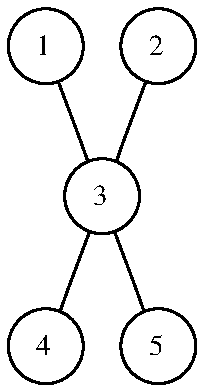
\includegraphics[scale=0.5]{g1.pdf}
    \caption{$S_n\ (n=5)$, exemple pour VC}
    $ $ \\
	$C = \{3\}$ est une solution réalisable. \\
	$VC(S_n)=1\ \forall n \geq 2$
    \end{center}
\end{figure}
\end{exemple}
\newpage
\begin{exemple}
Graphe complet à $n$ sommets, $K_n$.\\
\begin{figure}[h!]
    \begin{center}
    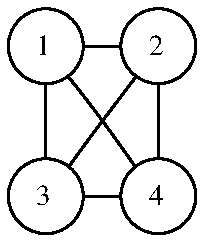
\includegraphics[scale=0.5]{g2.pdf}
    \caption{$K_n\ (n=4)$, exemple pour VC}
    $ $ \\
	$C = \{1,2,3\}$ est une solution réalisable. \\
	$VC(S_n)=n-1\ \forall n \geq 2$ \\
	Pour justifier cela, il suffit de voir que si on enlève toutes les arêtes
    concernant un sommet, on se retrouve à nouveau
	avec un graphe complet, on peut ainsi itérer récursivement jusqu'au cas de
    base $K_2$ où on sait que $VC(K_2) = 1$.
    \end{center}
\end{figure}
\end{exemple}

\begin{exemple}
Chemin à $n$ sommets, $P_n$.\\
\begin{figure}[h!]
    \begin{center}
    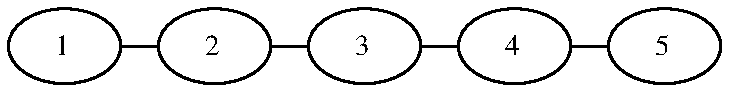
\includegraphics[scale=0.5]{pn.pdf}
    \caption{$P_n\ (n=5)$, exemple pour VC}
    $ $ \\
	$C = \{2,4\}$ est une solution réalisable. \\
	$VC(P_n)=\cdil{\frac{n}{2}}\ \forall n \geq 2$
    \end{center}
\end{figure}
\end{exemple}

\begin{exemple}
Cycle à $n$ sommets, $C_n$.\\
\begin{figure}[h!]
    \begin{center}
    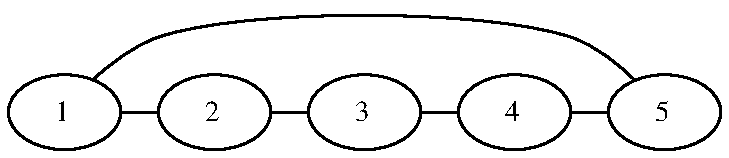
\includegraphics[scale=0.5]{cn.pdf}
    \caption{$C_n\ (n=5)$, exemple pour VC}
    $ $ \\
	$C = \{1,3,5\}$ est une solution réalisable. \\
	$VC(C_n)=\ceil{\frac{n}{2}}\ \forall n \geq 2$
    \end{center}
\end{figure}
\end{exemple}

\newpage

\begin{exemple}
Graphe biparti complet à $n+m$ sommets, $K_{n,m}$.\\
\begin{figure}[h!]
    \begin{center}
    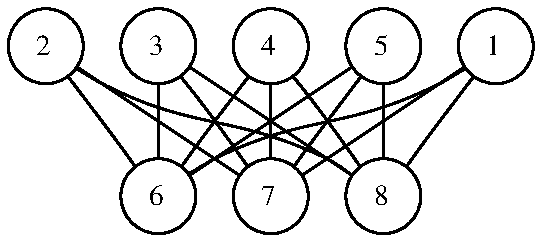
\includegraphics[scale=0.5]{knm.pdf}
    \caption{$K_{n,m}\ (n=5,\ m=3)$, exemple pour VC}
    $ $ \\
	$C = \{6,7,8\}$ est une solution réalisable. \\
	$VC(K_{n,m})=\min{(n,m)}\ \forall n,m \geq 1$
    \end{center}
\end{figure}
\end{exemple}

\begin{pblm} \textbf{MAX MATCHING (\titre{MM})}
\begin{itemize}
\item[*]\textbf{\underline{Instance}} : graphe $G=(V,E)$,
\item[*]\textbf{\underline{Solution}} : un ensemble d'arcs $F \subseteq E$ qui
est un \textit{matching}, c'est-à-dire qu'il n'y a pas 2 arêtes
\textit{incidentes} dans $F$ (extrémités communes).
\item[*]\textbf{\underline{Mesure}} : $|F|$
\end{itemize}
\end{pblm}

\begin{exemple} Valeurs pour \titre{MM} pour différents types de graphes :
\begin{itemize}
\item $MM(S_n) = 1$
\item $MM(C_n) = \cdil{\frac{n}{2}}$
\item $MM(P_n) = \cdil{\frac{n}{2}}$
\item $MM(K_{n,n}) = n$
\end{itemize}
\end{exemple}

\begin{rems}:
\begin{itemize}
\item Quand un graphe $G$ est biparti, $\titre{VC}(G) = \titre{MM}(G)$, sinon
$\titre{MM}(G) \leq \titre{VC}(G)$ avec égalité ssi $G$ est \textbf{biparti}.
\item \titre{VC} est \textbf{NP-Complet}, \titre{MM} ne l'est pas, c'est-à-dire
qu'il existe un algorithme polynomial pour calculer \titre{MM}. On va donc
pouvoir utiliser \titre{MM} pour approximer \titre{VC}.
\end{itemize}
\end{rems}

\subsection{Rappels et complexité des problèmes d'optimisation}
L'intuition que l'on suit est que \textbf{VERTEX COVER} est beaucoup plus
``difficile'' que \textbf{MAXIMUM MATCHING} (pour lequel il existe des
algorithmes polynomiaux).

\subsubsection*{Rappels}

\begin{itemize}
\item Un algorithme pour un problème est dit \textbf{polynomial} si le nombre
d'instructions pour résoudre ce problème peut être borné par un polynôme en la
taille de l'entrée.
\item Un \textbf{problème de décision} est un problème dont la sortie est soit
``Yes'' soit ``No''.
\item La classe $\mathcal{P}$ contient les problèmes de décisions qui admettent
des algorithmes polynomiaux pour les résoudre.
\item La classe $\mathcal{NP}$ est l'ensemble des problèmes de décision qui
peuvent être résolus en temps polynomial de manière non-déterministe
\textit{(c.f. cours de Calculabilité et Complexité)}.
\item De manière moins formelle, la classe $\mathcal{NP}$ est l'ensemble des
problèmes de décision tels que pour toute instance ``Yes'' il y a une preuve
``facile'' (algorithme polynomial) pour montrer que la réponse est ``Yes''
\textit{(c.f. métaphore avec la musique : ``Je suis capable de vérifier qu'une
musique est une bonne musique mais je suis incapable de la composer moi-même.'')
}.
\item Tout problème d'optimisation peut être exprimé sous la forme d'un problème
de décision. \\$ $\\
\begin{itemize}
\item[$\rightarrow$] Exemple : \\
\indent \hbox{\raisebox{0.4em}{\vrule depth 1pt height 0.4pt width 5cm}}
\begin{pbm}
\textbf{MIN VC-DECISION (\titre{VC-DEC})}
\begin{itemize}
\item[*]\textbf{\underline{Instance}} : Graphe $G=(V,E)$, $k \in \N$
\item[*]\textbf{\underline{Question}} : Existe-t-il une converture de $G$ de
taille $\leq k$?
\end{itemize}
\indent \hbox{\raisebox{0.4em}{\vrule depth 1pt height 0.4pt width 5cm}}
\end{pbm}
\item[$\rightarrow$] De manière générale, si $goal=min(\blu{max})$, demander,
pour un certain $k>0$, s'il existe une solution réalisable
$y$ pour une instance $x$ telle que $m(x,y) \leq (\blu{\geq}) k$ ($m$ étant
la mesure).
\end{itemize}
\end{itemize}

\subsection*{Définitions}
\begin{itemize}
\item Un problème de décision $A$ se \textbf{réduit polynomialement} en $B$,
noté $A\preceq B$, s'il existe un algorithme polynomial permettant de
transformer toute instance de $A$ en une instance de $B$ correspondante.
\item Un problème de décision $B$ est dit \textbf{$\mathcal{NP}$-complet} si
$B \in \mathcal{NP}$ et pour tout problème $A\ \mathcal{NP}$-complet, il existe
une réduction polynomiale $A\preceq B$.
\item Une \textbf{preuve par réduction} que $B$ est $\mathcal{NP}$-complet se
fait en 2 étapes :
\begin{enumerate}
\item Prouver que $B$ est dans $\mathcal{NP}$ \textit{(il faut donc prouver que
la vérification est polynomiale)};
\item Il existe un problème $A$ tel que $A\preceq B$ pour un problème $A$ connu
comme étant $\mathcal{NP}$-complet.
\end{enumerate}
\item Soit un problème de décision ou d'optimisation $A$. On dit qu'un
algorithme possède $A$ comme \textbf{oracle} si on suppose que l'algorithme peut
résoudre une instance de $A$ en une seule instruction ($O(1)$).
\item Un problème $A$ est \textbf{$\mathcal{NP}$-difficile}
\textit{($\mathcal{NP}$-hard)} s'il existe un algorithme polynomial pour un
problème $\mathcal{NP}$-complet $B$ quand cet algorithme possède $A$ comme
oracle. \\
\textit{(Intuition : Si $A$ était facile, alors $B$ le serait aussi})\\
\indent$\qquad$ Exemple : \textbf{VC} est $\mathcal{NP}$-difficile car si on
connait \textbf{VC(G)} en temps constant, alors le problème
\indent$\qquad\qquad\qquad\quad$\textbf{VC-décision} devient polynomial.
\end{itemize}

\subsection{Algorithmes d'approximation : qu'est-ce ? Pourquoi ?}
\begin{quote}\begin{center}
\textit{\quotecolor{{\Huge ``}}
\begin{Large}
\quotecolor{Probably close to optimal, but polynomial.}
\end{Large}
\quotecolor{{\Huge ''}}}
\end{center}\end{quote}

\subsubsection*{Définition}
Un \textbf{algorithme d'$\alpha$-approximation} pour un problème d'optimisation
est un algorithme polynomial qui \indent pour toutes les instances du problème
produit une solution dont la valeur est proche de la solution optimale \indent
à un facteur $\alpha$ près.

\subsubsection*{Remarques}
\begin{itemize}
\item On va suivre la convention suivante :
\begin{itemize}
\item[*]$\boxed{\alpha > 1}$ si \textbf{MIN}, par exemple, un algorithme de
$2$-approximation implique que la solution de l'algorithme est le double de
la solution optimale dans le pire des cas,
\item[*]$\boxed{\alpha < 1}$ si \textbf{MAX}, par exemple, un algorithme de
$\frac{1}{2}$-approximation implique que la solution de l'algorithme est la
moitié de la solution optimale dans le pire des cas.
\end{itemize}
\item $\alpha$ est la \textbf{garantie de performance}, aussi appelé
\textbf{facteur} ou \textbf{ratio d'approximation}.\\
Ce facteur n'est pas toujours constant, il peut dépendre de la taille de
l'entrée.
\end{itemize}

\subsubsection*{Pourquoi ?}
Nous donnons ici 6 raisons :
\begin{enumerate}
\item il y avait un certain besoin d'algorithmes pour obtenir des solutions
rapidement aux problèmes d'optimisation;
\item souvent la conception d'algorithmes se base sur des modèles idéalisés mais
peuvent donner des idées pour les "vrais"problèmes;
\item base mathématique rigoureuse pour étudier les heuristiques;
\item donne des garanties :
\begin{itemize}
\item à priori \textit{(facteur $\alpha$)},
\item à fortiori dans certains cas, \textit{(voir plus loin)};
\end{itemize}
\item donne un moyen de mesurer le niveau de difficultés des problèmes
d'optimisation;
\item c'est ``fun''.
\end{enumerate}

\subsubsection{Définitions}

\begin{itemize}
\item \textbf{Un schéma d'approximation en temps polynomial} \textit{(polynomial
time approximation scheme} (\textbf{PTAS})) est une famille d'algorithmes
$A_\epsilon$, où il y a un algorithme pour tout $\epsilon > 0$ tel que
$A_\epsilon$ est un algorithme de :
\begin{itemize}
\item[*] \textit{($1+\epsilon$)-approximation} si c'est une
\textbf{MIN}imisation,
\item[*] \textit{($1-\epsilon$)-approximation} si c'est une
\textbf{MAX}imisation.
\end{itemize}
$\qquad \rightarrow$ Exemple : problème du sac à dos et version euclidienne du
TSP (voyageur de commerce).

\item Il existe une classe (\textbf{MAX SNP}) de problèmes telle que :
\begin{thm} Pour tout problème \textit{$MAX SNP$-difficile}, il n'y a pas de
PTAS (sauf si $P = NP$).
\end{thm}

\item Il existe d'autres problèmes encore plus difficile. Par exemple :\\
\indent \hbox{\raisebox{0.4em}{\vrule depth 1pt height 0.4pt width 5cm}}
\begin{pbm} \textbf{MAX CLIQUE}
\begin{itemize}
\item[*]\textbf{\underline{Instance}} : graphe $G=(V,E)$,
\item[*]\textbf{\underline{Solution}} : un sous-ensemble de sommets $S
\subseteq V$ tel que $S$ est une \textbf{clique} \textit{(sous-graphe complet)},
\item[*]\textbf{\underline{Mesure}} : $|S|$
\end{itemize}
\indent \hbox{\raisebox{0.4em}{\vrule depth 1pt height 0.4pt width 5cm}}
\end{pbm}

\begin{thm}Soit $n = |V|$ et $0 < \epsilon < 1$ n'importe quelle constante,
alors il n'existe pas d'algorithme d'approximation avec un facteur
$O(n^{\epsilon-1})$ pour \textbf{MAX CLIQUE} \textit{(sauf si $P = NP$)}.
\end{thm}

\textbf{\underline{Commentaires}} :
\begin{enumerate}
\item si $\epsilon = 1$, $\exists$ un algorithme d'approximation en $O(1)$,
\item si $\epsilon = 0$, $\exists$ un algorithme d'approximation en
$O(\frac{1}{n})$,
\begin{itemize}
\item[$\rightarrow$] $OPT = n$ et $SOL = 1$ $\Rightarrow$ $\frac{SOL}{OPT} =
\frac{1}{n}$
\item[$\rightarrow$] \textbf{Algorithme idiot et très mauvais} mais
\rouge{\textbf{on ne peut pas faire mieux que lui !}} \\
\textit{Tout algorithme serait donc aussi bon que de prendre un seul sommet,
on ne peut pas améliorer ce facteur d'approximation.}
\end{itemize}
\end{enumerate}
\end{itemize}
\vspace{25em}
\begin{flushright}
$\hookrightarrow$ \begin{large}Voir exercices dans l'annexe~\ref{exochap1}.
\end{large}
\end{flushright}

\section{Set Cover et survol des techniques}

Ce problème possède diverses applications dans la vie de tous les jours. Par
exemple, les antivirus ou encore les ``\textit{Houses of Graphs}''.\\

\begin{pblm} \textbf{MIN SET\_COVER (\titre{SC})}
\begin{itemize}
\item[*]\textbf{\underline{Instance}} :
	\begin{itemize}
	\item Un ensemble $E = \{e_1, e_2, \ldots, e_n \}$ de $n$ éléments,
	\item des sous-ensembles $S_1$, $S_2$, $\ldots$, $S_m$ où chaque
    $S_j\subseteq E$,
	\item un poids non-négatif $w_j \geq 0$ pour chaque sous-ensemble $S_j$.
	\end{itemize}
\item[*]\textbf{\underline{Solution}} : Une collection $I$ de sous-ensembles qui
couvrent $E$. \\ C'est-à-dire $I\subseteq \{1,2,\ldots,n\}$ telle que
$\bigcup\limits_{j\in I}{S_j} = E$.
\item[*]\textbf{\underline{Mesure}} : $\sum\limits_{j\in I} w_j$
\end{itemize}
\end{pblm}

\begin{figure}[h!]
    \begin{center}
    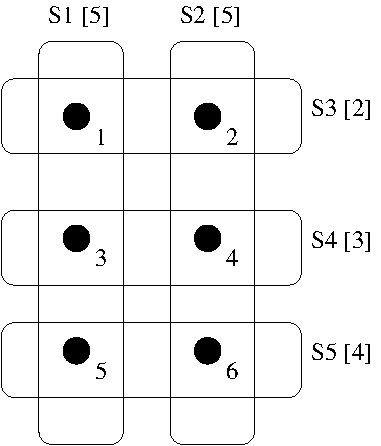
\includegraphics[scale=0.5]{inst_sc.pdf}
    \caption{Exemple d'instance de \titre{SC}}
    \end{center}
\end{figure}

$I_{OPT} = \{S_3,S_4,S_5\}$. \\
\indent Et si $w_j = 1, \forall j$ \textit{(version non-pondérée du problème)},
alors $I_{OPT} = \{S_1,S_2\}$.

\subsection{Programmation linéaire et Set Cover}

\begin{de}[Programme Linéaire]
Un programme linéaire (\titre{\textbf{PL}}) est spécifié par :
\begin{enumerate}
\item des variables de décision,
\item des contraintes sous la forme d'inégalités/égalités linéaires,
\item une fonction objectif linéaire.
\end{enumerate}
Un \textbf{\titre{PL} en nombres entiers (\titre{IP})} impose une contrainte
d'intégralité supplémentaire sur certaines variables.\\
Un \textbf{\titre{PL} 0-1} impose une contrainte supplémentaire de valeur
booléenne sur certaines variables.\\
\end{de}

\begin{propriete}
Un \textbf{\titre{PL}} où toutes les variables sont continues peut être résolus
en temps polynomial (non pas via le simplexe mais via la méthode des points
intérieurs ou via l'algorithme ellipsoïdale par exemple (il en existe
d'autres)).\\
\indent $\Rightarrow$ \textbf{Ils appartiennent donc à $\mathcal{P}$}. Un
\textbf{\titre{IP}} \textit{(Integer Programming)} par contre,
en général, est $\mathcal{NP}$-\textit{difficile}.
\end{propriete}

\begin{propriete}
Tout \textbf{\titre{IP}} peut être \textbf{relaxé}. \\
Par exemple : $x_j \in \{0,1\} \Rightarrow_{\text{relaxation}} x_j \geq 0$\\
(le $x_j \leq 1$ n'est pas utile car dès que c'est plus $0$, on sait qu'elle
n'est plus à la valeur booléenne $0$).
\end{propriete}
$ $\\$ $\\$ $\\$ $\\$ $\\$ $\\

Grâce à cette idée de relaxation on peut dégager un algorithme qui semble être
un algorithme d'approximation pour résoudre un problème \textbf{IP(*)} :
\begin{algorithm}[h!]
\caption{RelaxationApprox}
\begin{algorithmic}[1]
\STATE Résoudre le problème relaxé (\textbf{LP(**)})
\STATE Arrondir la solution optimale trouvée.
\end{algorithmic}
\end{algorithm}

Deux questions se posent alors: \textit{``Comment arrondir ?''} et
\textit{``Quel est le facteur $\alpha$ ?''}.\\
On sait que cet algorithme est polynomial si l'algorithme utilisé pour arrondir
est dans $\mathcal{P}$. \\
On sait également que \textbf{LP(**)} est une relaxation de \textbf{IP(*)}, ce
qui signifie que :
\begin{itemize}
\item toute solution réalisable d'\textbf{IP(*)} est une solution réalisable de
\textbf{LP(**)},
\item la valeur de toute solution réalisable dans \textbf{IP(*)} sera égale à la
même valeur dans \textbf{LP(**)}.
\end{itemize}
$\Rightarrow$ \textbf{LP(**)} a plus de solutions réalisables que
\textbf{IP(*)}.\\
En d'autres mots, dans le cas d'une \textbf{MIN}imisation, si :
\begin{itemize}
\item $Z^*_{LP}$ est la solution optimale pour le \textbf{LP}
\item $Z^*_{IP}$ est la solution optimale pour le \textbf{IP}
\end{itemize}
alors on a $\boxed{Z^*_{LP} \leq Z^*_{IP} = OPT}$.

\begin{exemple}$ $\\
$\max\ x_1+x_2$ \\
\indent $\text{\textbf{s.l.c }} 4x_1 + 3x_2 \leq 12\ (1)$ \\
\indent	$\qquad 2x_1 + 5x_2 \leq 10\ (2)$ \\
\indent $\qquad\ x_1, x_2 \in \N$

\begin{figure}[h!]
    \begin{center}
\setlength{\unitlength}{1.0cm}
\begin{picture}(6,5)(0,0)
% AXES
\linethickness{0.3mm}
\put(0, 0){\vector(0,1){5}}
\put(0, 0){\vector(1,0){6}}
% GRADUATIONS
\put(0, 4){\line(-1,0){0.1}}
\put(0, 3){\line(-1,0){0.1}}
\put(0, 2){\line(-1,0){0.1}}
\put(0, 1){\line(-1,0){0.1}}
\put(-0.4, 3.9){$4$}
\put(-0.4, 1.9){$2$}
\put(5,0) {\line(0,-1){0.1}}
\put(4,0) {\line(0,-1){0.1}}
\put(3,0) {\line(0,-1){0.1}}
\put(2,0) {\line(0,-1){0.1}}
\put(1,0) {\line(0,-1){0.1}}
\put(2.9,-0.4){$3$}
\put(4.9,-0.4){$5$}
% DROITES
\put(0, 4){\color{darkblue} \line(3, -4){3}}
\put(1, 3){\blu{$(1)$}}
\put(0, 2){\color{magenta} \line(5, -2){5}}
\put(4, 0.5){\textcolor{magenta}{$(2)$}}
% POINTS
\put(0,0){\color{green} \circle*{0.1}}
\put(0,1){\color{green} \circle*{0.1}}
\put(0,2){\color{green} \circle*{0.1}}
\put(1,0){\color{green} \circle*{0.1}}
\put(1,1){\color{green} \circle*{0.1}}
\put(2,0){\color{green} \circle*{0.1}}
\put(2,1){\color{green} \circle*{0.1}}
\put(3,0){\color{green} \circle*{0.1}}
% Z*_LP
\put(2.142857143,1.142857143) {\color{darkred} \circle*{0.15}}
\put(2.242857143,1.242857143) {\rouge{$Z^*_{LP}$}}
% Z*_IP
\put(2,1){\color{green} \circle*{0.15}}
\put(1.5,0.7){\gre{$Z^*_{IP}$}}
\end{picture}
    \end{center}
\end{figure}
\end{exemple}

$\rightarrow Z^*_{LP} = (\frac{15}{7},\frac{8}{7}) \simeq (2,1) = Z^*_{IP}$ \\
\indent \textit{(on a de la chance on trouve la solution optimale via notre
algorithme polynomial).}

\subsubsection*{Solution pour l'arrondi \titre{SC}}

Posons $f$ comme le nombre maximum de sous-ensembles dans lesquels n'importe
quel élément apparaît,
$$f = \max_{i=1,\ldots,n}{(f_i)}\text{ où }f_i = \left| \{j : e_i \in S_j \}
\right|$$

Soit $x^* = (x_1^*, x_2^*, .. x_n^*)$ la solution optimale du \textbf{LP},
on va arrondir en incluant $S_j$ dans la solution si et seulement si
$x_j^* \geq \frac{1}{f}$.

\begin{thm}
Cette manière de procéder est un algorithme de $f$-\textit{approximation}.
\end{thm}
\begin{corollaire}
L'adaptation de cet algorithme donne un algorithme de $2$-approximation pour le
\titre{VC}.
\end{corollaire}

\vspace{5em}

\begin{algorithm}[h!]
\caption{Det\_Rounding\_SC}
\begin{algorithmic}[1]
\STATE Résoudre le \textbf{LP} pour \textbf{\titre{SC}}
\STATE Soit $x^*$ la solution optimale pour \textbf{LP}
\STATE A partir de $x^* = (x^*_1,x^*_2, \ldots, x^*_m)$,\\
on inclut $S_j$ dans la solution ``arrondie'' ssi $x^*_j \geq \frac{1}{f}$
\end{algorithmic}
\end{algorithm}

où $f = \max_{i=1,...,n} (f_i)$ où $f_i = |\{j:e_i \in S_j\}|$ et $I =$ ensemble
des indices sélectionnés.

\begin{lemme}
La collection des $S_j$, $j \in I$ est une couverture.
\begin{proof}
On va montrer que tout $e_i$ est couvert.\\
Comme $x^*$ \textit{(la solution optimale du \textbf{LP})} est une solution
réalisable, on a :
$$\sum_{j : e_i\in S_j} (x^*_j) \geq 1\text{ pour un certain } e_i.$$
\begin{center}\textit{(une contrainte pour un élément donné)}\end{center}
Par définition, $f_i \leq f$, on a donc au maximum $f$ termes dans la somme. \\
Donc, il y a au moins un terme $x^*_j$ qui doit être $\geq \frac{1}{f}$ car si
ils sont tous $<\frac{1}{f}$, la somme n'est pas $\geq 1$.\\
$\Rightarrow$ Il existe un $j$ tel que $e_i \in S_j$ et $x^*_j \geq \frac{1}{f}$.
En conséquence, $j \in I$ par l'algorithme et $e_i$ est couvert.
\cqfd
\end{proof}
\end{lemme}

\begin{thm} Det\_Rounding\_SC est un algorithme de $f$-\textit{approximation}
pour \textbf{\titre{SC}}.
\begin{proof}
On voit que l'algorithme est polynomial.\\
Prouvons que la solution approché est égale à $f$ fois la solution optimale,
càd:
$$ \sum_{j\in I} w_j = APP \leq f * OPT  $$
Par construction, $1 \leq f*x^*_j,\ \forall j \in I$. \textbf{(**)}\\
Ensuite,
\begin{eqnarray}
\sum_{j\in I} (w_j) & \leq & \sum_{j=1}^m (w_j.1) \\
				    & \leq & \sum_{j=1}^m w_j . f . x^*_j
                    \text{ (par \textbf{(**)})} \\
				    &   =  & f \sum_{j=1}^m w_j . x^*_j \\
				%	&   =  & \text{($f \times$ valeur de la fonction objective pour la solution optimale du LP)} \\
					&   =  & f \cdot Z_{LP}^* \\
					& \leq & f \cdot OPT
\end{eqnarray}
\cqfd
\end{proof}
\end{thm}

Le facteur $f$ ainsi calculé est une \textbf{garantie à priori}, c'est-à-dire
qu'avant même de lancer l'algorithme, on est sûr que ce facteur d'approximation
sera vérifié. Cependant, l'algorithme \textbf{Det\_Rounding\_SC} permet d'avoir
également une \textbf{garanti à fortiori}, c'est-à-dire une garantie que l'on a
lorsque on a commencé à exécuter l'algorithme (dans ce cas-ci, lorsque l'on a
la réponse au problème relaxé). En effet, prenons
$\alpha = \frac{\sum_{j\in I}(w_j)}{Z^*_{LP}}$, de la preuve précédente on a que
$\sum_{j\in I}(w_j) \leq f.Z^*_{LP}$ et donc $\alpha \leq f$ (dans certain cas,
$\alpha$ peut être beaucoup plus petit que $f$). On a également
$\frac{APP}{OPT}\leq \alpha$, ce qui fait d'$\alpha$ un meilleur facteur
d'approximation que $f$ bien qu'il ne soit calculable qu'à partir de la solution
obtenue via la résolution du problème relaxé ($Z^*_{LP}$).

\vspace{4em}

\begin{exemple}[Voir feuilles des résultats obtenus avec CPLEX]$ $\\
\textbf{\titre{SC}} : $\alpha = \frac{9}{9} = 1$ \\
\textbf{\titre{VC}} : $APP = 5$, $Z^*_{LP} = 2.5 \Rightarrow \alpha = 2$. \\
\begin{multicols}{2}
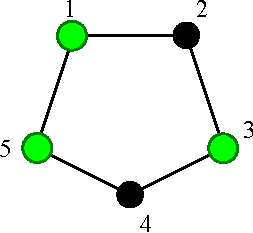
\includegraphics[scale=1]{vcSol.pdf}
$ $\\$ $\\$ $\\$ $\\
$OPT = 3$\\
$5 \leq 2*3=6$
\end{multicols}
\end{exemple}

\begin{corollaire}
L'algorithme \textbf{Det\_Rounding\_SC} peut être adapté au \textbf{\titre{VC}}
pour donner algorithme de 2-approximation (vu que $f = 2$ pour
\textbf{\titre{VC}}).
\end{corollaire}

\subsection{Primal $\leftrightarrow$ Dual}

\begin{de}[Problème dual]
Pour tout \textbf{\titre{LP}}, il existe un autre \textbf{\titre{LP}} appelé son
\textbf{dual} qui possède des propriétés intéressantes.
\end{de}

\begin{exemple}
Voir feuilles des résultats obtenus avec \textbf{CPLEX}.
\end{exemple}

L'intuition du \textbf{dual} est que l'on se met à la place de
l'\textit{entrepreneur} tandis que le \textbf{primal} correspond au point de vue
du \textit{client}. \\

Pour le \textbf{\titre{SC}}, chaque élément $e_i$ est \textit{``facturé''} d'un
prix $y_i \geq 0$ à payer pour le couvrir. Pour que les prix soient
raisonnables,
$$\sum_{i:e_i\in S_j} (y_i) \leq w_j\ (\forall j \in \{1,...,m\})$$
c'est-à-dire, en français que l'on n'accepte pas que la somme des prix à payer
pour couvrir les éléments d'un ensemble $S_j$ soit supérieur au poids de cet
ensemble. Le problème \textbf{dual} est défini comme suit :\\

$\max\ \sum_{i=1}^n y_i$ \\
\indent s.l.c.
\begin{itemize}
\item $\sum_{i:e_i \in S_j}(y_i) \leq w_j\, (\forall j \in \{1,\ldots ,m\})$ \\
\item $\qquad\ y_i \geq 0\, (\forall i \in \{1,\ldots ,n\})$
\end{itemize}

\subsubsection{Remarques et propriétés du dual}

\begin{rems}
\begin{itemize}
\item On appelle le \textbf{\titre{LP}} ``original'' le
\textbf{problème primal}.
\item Le \textbf{dual} du \textbf{dual} est le \textbf{primal}.
\item A chaque variable du \textbf{dual} correspond une contrainte du
\textbf{primal}.
\item A chaque variable du \textbf{primal} correspond une contrainte du
\textbf{dual}.
\end{itemize}
\end{rems}

\begin{thm}[\titre{Dualité faible}] Soit $x$ une solution réalisable du primal
(\textbf{MIN}) et $y$ une solution réalisable du dual (\textbf{$\Rightarrow$
MAX}), alors la valeur de $y \leq$ la valeur de $x$ (et $\geq$ si le primal est
une \textbf{MAX} et le dual une \textbf{MIN}).
\end{thm}

\begin{exemple}[Set Cover]
$$\sum_{i=1}^n(y_i) \leq \sum^m_{j=1} (x_j.w_j)$$
\end{exemple}

\begin{thm}[\titre{Dualité forte}] S'il existe des solutions qui sont
réalisables pour le primal \textbf{ET} pour le dual alors \textbf{les valeurs
optimales de ces 2 problèmes sont égales}.
\end{thm}

\begin{exemple}[Set Cover]
$x^*$ et $y^*$ sont des solutions optimales pour respectivement le
\textbf{primal} et le \textbf{dual} alors :
$$ \sum_{i=1}^n y^*_i = \sum_{j=1}^m x^*_j.w_j$$
\end{exemple}

\begin{algorithm}[h!]
\caption{Dual\_Rounding\_SC}
\begin{algorithmic}[1]
\STATE Résoudre le \textbf{dual} pour \textbf{\titre{SC}}
\STATE Soit $y^*$ la solution obtenue
\STATE Sélectionner $j$ dans $I'$ si l'inégalité correspondante dans le
\textbf{dual} est serrée \textit{(donc l'égalité)}.\\
\textit{(c'est-à-dire $\sum_{i : e_i \in S_j} (y^*_i) = w_j$)}
\end{algorithmic}
\end{algorithm}

\begin{exemple}[Set Cover] (Voir feuilles des résultats obtenus avec
\textbf{CPLEX}) \\
$y^* = (0,2,0,3,4,0)$ \\
$I = \{2,3,4,5\}$ (les contraintes serrées sont $c_2$, $c_3$, $c_4$ et $c_5$)\\
$APP=9+5=14$.
\end{exemple}

\begin{exemple}[Vertex Cover] (Voir feuilles des résultats obtenus avec
\textbf{CPLEX}) \\
$I' = \{1,2,3,4,5\}$
\end{exemple}

On peut montrer que cette $2^{\text{ème}}$ approche ne fait jamais mieux que la
première. En effet, $I \subseteq I'$ c'est-à-dire que les indices sélectionnés
par \textbf{Det\_Rounding\_SC} est un sous-ensemble des indices sélectionnés par
\textbf{Dual\_Rounding\_SC}.

\begin{lemme}
La collection des $S_j$ tq $j\in I'$ est une couverture.$ $\\
\begin{proof}[par l'absurde]
Supposons qu'il existe $e_k$ qui n'est pas couvert par les sous-ensembles $S_j$,
$j\in I'$.\\
Donc, par construction, et pour tout ensemble $S_j$ contenant $e_k$ :
$$\sum_{i : e_i \in S_j}(y^*_i) < w_j $$
\begin{center}
\textit{(contrainte non serrée, sinon on aurait sélectionné $S_j$)}
\end{center}

On définit $\epsilon$ comme la plus petite différence entre le \textbf{membre
droit} \textit{(rhs)} et le \textbf{membre gauche}
\textit{(lhs)} des contraintes/inégalités impliquant $e_k$.
C'est-à-dire
$\epsilon = \min_{j:e_k \in S_j} {(w_j - \sum_{i : e_i \in S_j} y^*_i)}$.
$\Rightarrow$ On a que $\boxed{\epsilon > 0}$. \\

On définit à présent
\begin{eqnarray}
y'_k & = & y^*_k+\epsilon \\
y'_i & = & y^*_i\qquad\qquad \forall i \neq k
\end{eqnarray}
$\Rightarrow y'$ est une solution réalisable car
\begin{itemize}
\item pour tout $j$ t.q. $e_k \in S_j$ :
$$\sum_{i:e_i\in S_j} y'_i = \sum_{i:e_i\in S_j}(y^*_i+\epsilon) \leq w_j$$
\begin{center} \textit{(par définition de $y'k$)} \end{center}
\item pour tout $j$ t.q $e_k \not\in S_j$ :
$$\sum_{i:e_i\in S_j} y'_i = \sum_{i:e_i\in S_j}(y^*_i) \leq w_j$$
\end{itemize}
Pourtant $\sum y'_i > \sum y^*_i \Rightarrow$ $y'$ est meilleure que la solution
optimale.
\contrad
\end{proof}
\end{lemme}

\begin{thm} L'algorithme \textbf{Dual\_Rounding\_SC} est un algorithme
d'approximation de facteur $f$.
\begin{proof}\textit{(idée)}
\noindent \begin{itemize}
\item[*] Quand on choisit un ensemble $S_j$ dans la couverture, on ``paye'' en
facturant $y^*_i$ \\ à chacun de ses éléments $i$.
\item[*] Chaque élément est facturé au plus une fois pour chaque ensemble qui
le contient \\ \textit{(et donc au plus $f$ fois, par définition de $f$)}.
\item[*] Le coût total est au plus $f$ fois le cout de la solution optimale,
c'est-à-dire \textit{(dualité forte)}:
$$\text{COUT\_TOTAL} = f.\sum_{i=1}^n(y^*_i) = f.Z^*_{LP} \leq f.OPT$$
\end{itemize}
\end{proof}
\end{thm}

\subsection{La méthode primale-duale}

\noindent On a vu 2 algorithmes avec facteur $f$ (sections 2.1 et 2.2) mais ils
nécessitent de résoudre un \textbf{\titre{LP}}.\\
\indent $\Rightarrow$ On va utiliser la preuve du lemme de la section 2.2
\textit{(dual rounding)} pour en tirer un algorithme.

\begin{algorithm}[h!]
\caption{Primal\_Dual\_SC}
\begin{algorithmic}[1]
\STATE $\forall i,\ y_i \leftarrow 0$
\STATE $I\leftarrow \{\}$
\WHILE{il existe un $e_i$ non couvert}
\FOR{chaque $S_k \ni e_i$}
\STATE $\Delta_k \leftarrow w_k - \sum_{j:e_j\in S_k}(y_j)$
\ENDFOR
\STATE $l \leftarrow arg\min_{k:e_i\in S_k}(\Delta_k)$
\STATE $y_i \leftarrow y_i+\Delta_l$
\STATE $I\leftarrow I\cup \{l\}$
\ENDWHILE
\end{algorithmic}
\end{algorithm}

\begin{rem}
$arg\min_{i\in A}(x_i)$ donne le $k$ tel que $x_k$ est le minimum des $x_i$.
\end{rem}

\begin{exemple}
Voir section $1.4$ de la feuille ``Resultats obtenus avec CPLEX''. Appliquons
l'algorithme : \\
\indent $y \leftarrow 0$, $I \leftarrow \{\}$
\begin{itemize}
\item \textbf{Itération $1$} ($e_i = e_1$) :\\
on considère toutes les contraintes $c_k$ correspondant aux $S_k \ni e_1$ et on
calcule $\Delta_k$ :
	\begin{itemize}
	\item $c_1\ :\ y_1+y_3+y_5 \leq 5\ \Leftrightarrow 0+0+0\leq 5 \Rightarrow
    \Delta_1 = 5$
	\item $c_3\ :\ y_1+y_2 \leq 2\ \Rightarrow \Delta_3 = 2$
	\end{itemize}
	$\hookrightarrow l = 3$ \\
	$\hookrightarrow y = (2,0,0,0,0,0)$\\
	$\hookrightarrow I = \{3\}$\\
\item \textbf{Itération $2$} ($e_i = e_3$ car $e_2$ est couvert par $S_3$) :\\
on considère toutes les contraintes $c_k$ correspondant aux $S_k \ni e_3$ et on
calcule $\Delta_k$ :
	\begin{itemize}
	\item $c_1\ :\ 2+y_3+y_5 \leq 5\ \Rightarrow \Delta_1 = 3$
	\item $c_4\ :\ y_3+y_4 \leq 3\ \Rightarrow \Delta_4 = 3$
	\end{itemize}
	$\hookrightarrow l = 1$ (choix aléatoire ici)\\
	$\hookrightarrow y = (2,0,3,0,0,0)$\\
	$\hookrightarrow I = \{1,3\}$\\
\item \textbf{Itération $3$} ($e_i = e_4$) :\\
on considère toutes les contraintes $c_k$ correspondant aux $S_k \ni e_4$ et on
calcule $\Delta_k$ :
	\begin{itemize}
	\item $c_2\ :\ y_2+y_4+y_5 \leq 5\ \Rightarrow \Delta_2 = 5$
	\item $c_4\ :\ 3+y_4 \leq 3\ \Rightarrow \Delta_4 = 0$
	\end{itemize}
	$\hookrightarrow l = 4$\\
	$\hookrightarrow y = (2,0,3,0,0,0)$\\
	$\hookrightarrow I = \{1,3,4\}$ \\
\item \textbf{Itération $4$} ($e_i = e_6$) :\\
on considère toutes les contraintes $c_k$ correspondant aux $S_k \ni e_6$ et on
calcule $\Delta_k$ :
	\begin{itemize}
	\item $c_2\ :\ \ldots\ \Rightarrow \Delta_2 = 5$
	\item $c_5\ :\ \ldots\ \Rightarrow \Delta_4 = 0$
	\end{itemize}
	$\hookrightarrow l = 5$\\
	$\hookrightarrow y = (2,0,3,0,0,4)$\\
	$\hookrightarrow I = \{1,3,4,5\}$
\end{itemize}
\indent$\quad$ \textbf{fin.} \textit{(tout est couvert)}
\end{exemple}

\begin{rem}
Cet algorithme est intéressant car il est simple à implémenter et qu'il ne
nécessite pas de résoudre le \titre{\textbf{LP}}.
\end{rem}

\begin{thm}
L'algorithme Primal\_Dual\_SC est un algorithme de $f$-approximation.
\end{thm}

\subsection{Algorithme d'approximation glouton}

\begin{algorithm}[h!]
\caption{Greedy\_SC}
\begin{algorithmic}[1]
\STATE $i\leftarrow \{\}$
\STATE $\forall j,\ \hat{S}_j \leftarrow S_j$ \textit{// Cette variable
représente les éléments non-couverts de $S_j$}
\WHILE{$I$ n'est pas une couverture}
\STATE $l\leftarrow arg\min_{j:\hat{S}_j \neq \{\}} \dfrac{w_j}{|\hat{S}_j|}$
\STATE $I \leftarrow I\cup \{l\}$
\STATE $\forall j,\ \hat{S}_j \leftarrow \hat{S}_j \setminus S_l$
\ENDWHILE
\end{algorithmic}
\end{algorithm}

\begin{exemple} Appliquons l'algorithme :\\
\begin{multicols}{2}
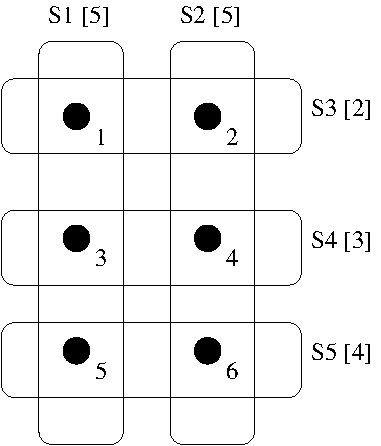
\includegraphics[scale=0.5]{inst_sc.pdf}
\begin{itemize}
\item[] $I \leftarrow \{\}$
\item[] $\hat{S}_j \leftarrow S_j$
\item[] \textbf{iteration 1} : $l = 3\ \left(\dfrac{2}{2} < \dfrac{3}{2} <
\dfrac{5}{3} = \dfrac{5}{3} < \dfrac{4}{2}\right)$
\item[] \textbf{iteration 2} : $l = 4\ \left(\dfrac{3}{2} < \dfrac{4}{2} <
\dfrac{5}{2} = \dfrac{5}{2}\right)$
\item[] \textbf{iteration 3} : $l = 5\ \left(\dfrac{4}{2} < \dfrac{5}{1} <
\dfrac{5}{1}\right)$
\item[] $I \leftarrow \{3,4,5\}$ $\Longrightarrow$ \textbf{solution optimale !}
\end{itemize}
\end{multicols}
\end{exemple}

Cet algorithme est beaucoup plus simple et en fait le meilleur pour
\textbf{\titre{SC}} \textit{(on peut pas faire meilleur algorithme
d'approximation)} mais ce qu'on gagne en simplicité dans l'algorithme, on va le
perdre dans le calcul du facteur d'approximation.

\begin{rappel}
Pour le \textbf{\titre{VC}}, nous avons déjà appliqué ce type d'algorithme.
Pour rappel, il donnait un facteur d'approximation $\sim\log{k}$ ce qui n'est
pas un facteur borné. Cet algorithme ne donne donc pas toujours de très bons
résultats mais c'est en général assez bon.
\end{rappel}

\begin{interlude}[Nombre harmonique]
On note $H_k$ le $k^{\text{ème}}$ nombre harmonique qui est calculé comme :
$$ H_k = 1 + \frac{1}{2} + \frac{1}{3} + \frac{1}{4} + \ldots + \frac{1}{k} =
\sum_{i=1}^k \frac{1}{i} \sim \ln{(k)} $$

\begin{center}
\begin{tabular}{|l|l|l|l|l|l|l|l|l|l|}
\hline
$k$		& $1$ & $2$	& $3$ 	  & $\ldots$ & $6$    & $\ldots$ & $100$  & $\ldots$
& $10000$ \\
\hline
$H_k$		& $1$ & $1.5$  & $1.83$ & $\ldots$ & $2.45$ & $\ldots$ & $5.19$
& $\ldots$ & $9.79$ \\
\hline
$\ln{(k)}$	& $0$ & $0.69$ & $1.09$ & $\ldots$ & $1.79$ & $\ldots$ & $4.6$
& $\ldots$ & $9.21$ \\
\hline
\end{tabular}
\end{center}
\end{interlude}

\newpage

\begin{thm}L'algorithme \textbf{Greedy\_SC} est un algorithme
d'$H_n$-approximation où $n$ est le nombre d'éléments à couvrir.
\begin{proof}$ $\\
\begin{itemize}
\item L'algorithme est \textbf{polynomial} car $O(m)$ itérations (à chaque
itération on sélectionne un sous-ensemble et il y en a maximum
$m$) et pour chaque itération, un travail en $O(m)$ est effectué (calcul des
ratios et du minimum) $\Rightarrow O(m^2)$.
\item On définit :
	\begin{itemize}
	\item[$\blacktriangle$] $n_k$ comme le nombre d'éléments non-couverts au
    début de la $k^{\text{ème}}$ itération,
	\item[$\blacktriangle$] $l$ comme le nombre d'itérations utilisées pour
    \textbf{Greedy\_SC},\\
	$\Rightarrow$ ainsi,
		\begin{itemize}
		\item[$\vartriangle$] $n_1 = n$
		\item[$\vartriangle$] $n_{l+1} = 0$
		\item[\rouge{$\blacktriangle$}] \rouge{$\mathbf{n_k > n_{k+1}}$
        \textbf{(*)}}
		\end{itemize}
	\item[$\blacktriangle$] $I_k$ (pour une itération $k$) comme l'indice des
    ensembles sélectionnés jusque là (donc lors des itérations
	$1$, $\ldots$, $k-1$),
	\item[$\blacktriangle$] $\hat{S}_j$ comme l'ensemble des éléments non
    couverts dans $S_j$ au début de l'itération $k$,
	$$\hat{S}_j = S_j - \bigcup_{p\in I_k}{S_p}$$
	\end{itemize}
\item On suppose que (on le prouvera par après), pour l'ensemble $S_j$ choisi à
l'itération $k$ :
$$ w_j \leq \frac{(n_k - n_{k+1})}{n_k}OPT = \frac{|\hat{S}_j|}{n_k}OPT\
\text{\textbf{(1)}}$$
\item Sous l'hypothèse que \textbf{(1)} est vraie, on a :
$$ \begin{eqnarray}
APP & = & \sum_{j\in I}(w_j) \leq \sum_{k=1}^l \frac{(n_k -n_{k+1})}{n_k}OPT\\
	& = & OPT \sum_{k=1}^l \frac{(n_k -n_{k+1})}{n_k}\\
	& = & OPT \sum_{k=1}^l \left(\frac{1}{n_k} + \frac{1}{n_k} + \ldots +
	  \frac{1}{n_k}\right) \text{ (car $n_k > n_{k+1}$)}\\
	& \leq & OPT \sum_{k=1}^l \left(\frac{1}{n_k} + \frac{1}{(n_k-1)} +\ldots +
          \frac{1}{(n_{k+1}+1)}\right)\\
	& = & OPT \sum_{i=1}^l \frac{1}{i} \\
	& = & OPT.H_l
\end{eqnarray}$$ $$\Rightarrow \frac{APP}{OPT} \leq H_n$$
\begin{exemple}($n_k=6$ et $n_{k+1}=2$) \\
$\frac{n_k - n_{k+1}}{n_k}=\frac{6-2} 6 \leq \frac 1 6 +\frac 1 6 +\frac 1 6 +
\frac 1 6 \leq \frac 1 6 +\frac 1 5 +\frac 1 4 +\frac 1 3$
\end{exemple}
\end{itemize}
\end{proof}
\end{thm}

Il ne reste donc qu'à prouver l'inégalité \textbf{(1)}. \\

\newpage

\begin{proof}[$w_j \leq \frac{(n_k - n_{k+1})}{n_k}OPT$]$ $\\
A l'itération $k$, on a
$$ \min_{j:\hat{S}_j \neq \{\}} \left(\frac{w_j}{|\hat{S}_j|}\right) \leq
\frac{OPT}{n_k}\qquad \text{\textbf{(2)}}$$
On observe :
\begin{itemize}
\item il existe une solution optimale qui couvre $n$ éléments pour un coût
\textbf{OPT},
\item au début, il existe un sous-ensemble qui couvre ses éléments avec un poids
moyen $\frac{w_j}{|S_j|} \leq \frac{OPT}{n}$
\item de manière similaire, quand $p$ éléments ont été couverts, à l'itération
$k$, la même solution \textbf{OPT} peut couvrir les
$n-p$ éléments non-couverts avec poids $\leq$ \textbf{OPT}.
\end{itemize}
$\Rightarrow$ il existe un sous ensemble qui couvre ses propres éléments
non-couverts avec un poids $\leq \frac{OPT}{n-p}$ et $n-p = n_k$ $\Rightarrow$
\textbf{(2)} est prouvée. \\

\noindent Donc, on choisit $S_j$ à l'itération $k$ tel que:
$\frac{w_j}{|\hat{S}_j|} \leq \frac{OPT}{n_k}$ (par \textbf{(2)}).\\
$\Longrightarrow$ Il y aura donc $|\hat{S}_j|$ éléments nouvellement couverts ce
qui signifie $n_{k+1} = n_k-|\hat{S}_j| $. \\
Dès lors $\dfrac{w_j}{|\hat{S}_j|} \leq \frac{OPT}{n_k}$ devient
$$w_j \leq \frac{(OPT.|\hat{S}_j|)}{n_k} = \frac{(n_k-n_{k+1})}{n_k}.OPT$$

\cqfd
\end{proof}

\begin{thm} L'algorithme \textbf{Greedy\_SC} est un algorithme de
$H_g$-approximation où $g = \max_{j}(|S_j|)$\\ ($g$ est en fait le maximum
d'éléments dans un sous-ensemble).
\end{thm}

\subsection{Conclusion du chapitre}

On a testé plusieurs types d'algorithmes d'approximation et on peut en conclure
qu'il n'y en a pas un qui est meilleur que tous les autres, cela dépendant des
instances \textit{(bien que pour le \titre{\textbf{SC}} on a très peu d'espoir
de faire mieux que l'algorithme glouton)}. On terminera cette section par
l'énoncé d'un résultat bien connu sur lequel on va se baser pour conjecturer
que $\mathcal{P} \neq \mathcal{NP}$.

\begin{thm}[Hardness result]
Sous l'hypothèse que la conjecture ``jeux uniques'' (conjecture disant que le
problème des ``jeux uniques'' est $\mathcal{NP}$-difficile, ce qui n'est pas
encore prouvé) est vraie et s'il existe un algorithme
d'$\alpha$-approximation (général, évidemment) pour \textbf{\titre{VC}} avec
$\alpha < 2$, alors $\mathcal{P} = \mathcal{NP}$.
\end{thm}

\vspace{22em}
\begin{flushright}
$\hookrightarrow$
\begin{large}Voir exercices dans l'annexe~\ref{exochap2}.\end{large}
\end{flushright}

\newpage

\section{Algorithmes gloutons et de recherche locale}

Pour rappel, on a utilisé ce type d'algorithme au chapitre 2 pour résoudre le
\textbf{\titre{SC}} avec un facteur d'approximation de $H_n$ (et même $H_g$).
Dans ce chapitre nous allons changer d'approche, au lieu de définir un problème
et d'utiliser plusieurs approches pour l'approximer, nous allons voir plusieurs
problèmes que l'on va uniquement considérer via l'approche gloutone ou de la
recherche locale. Mais qu'est-ce exactement un algorithme glouton ? et un
algorithme de recherche locale ?

\begin{de}[Algorithme glouton]
Algorithme où la solution est construite \textbf{pas à pas}. A chaque pas la
\textbf{partie} suivante est construite en prenant une décision qui est
localement la meilleure possible.
\end{de}

\begin{exemple}[Chapitre 2] \textbf{Greedy\_SC} est un algorithme où le choix
local consiste à prendre le sous-ensemble avec le meilleur ratio
$\dfrac{poids}{\#\text{éléments que l'on couverait en prenant le sous-ensemble}
}$.
\end{exemple}

\begin{de}[Algorithme de recherche locale]
\begin{multicols}{2}
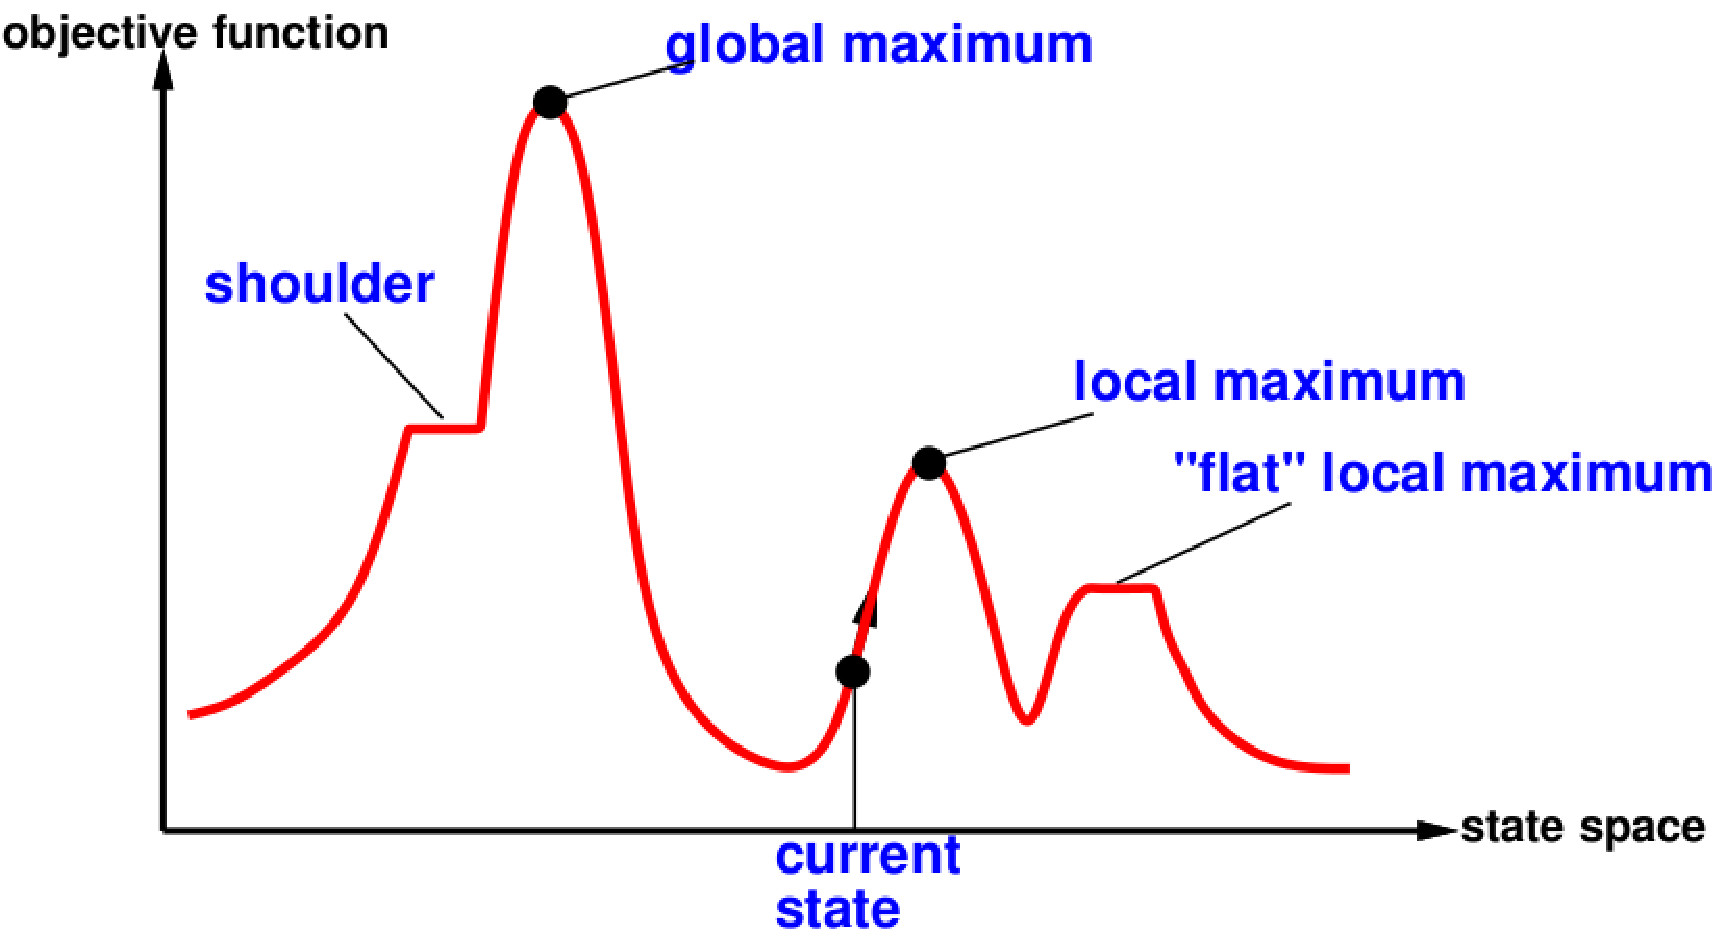
\includegraphics[scale=0.25]{graphique.pdf}
$ $\\$ $\\$ $\\$ $\\
Algorithme commençant avec une \textbf{solution initiale réalisable} qui est
améliorée \textbf{pas à pas} en considérant le \textbf{voisinage} de cette
solution. Dès que ce n'est plus possible, l'algorithme s'arrête.
\end{multicols}
\end{de}
Comme on peut le voir sur le dessin, si on est bloqué dans un optimum local,
on obtient une solution qui n'est pas l'optimum global.
\begin{exemple}[Chapitre 2]
Pour le \textbf{\titre{SC}} on peut prendre comme voisinage
``Sélectionner un ensemble et en désélectionner un autre''.
\end{exemple}

\subsection*{Comparaison}

\begin{enumerate}
\item Les points communs :
	\begin{itemize}
	\item ils prennent tous deux des décisions qui optimisent un choix local,
	\item la solution obtenue est une solution approchée,
	\item ils sont très facilement implémentables $\rightarrow$ ils sont souvent
    très populaires.
	\end{itemize}
\item Les différences :
	\begin{itemize}
	\item \begin{itemize}
		   \item[\textbf{Glouton} :] solution partielle qui sera réalisable à la
           fin,
		   \item[\textbf{Recherche locale} :] solution réalisable tout au long
           de l'exécution;
		  \end{itemize}
	\item \begin{itemize}
		   \item[\textbf{Glouton} :] souvent évident de prouver que l'algorithme
           est polynomial,
		   \item[\textbf{Recherche locale} :] rarement polynomial avec une
           implémentation simple mais dans certains cas elle l'est. Ces cas
           nécessitent en général certaines restrictions sur les changements
           possibles pour assurer un temps polynomial.
		  \end{itemize}
	\end{itemize}
\end{enumerate}

\newpage

\subsection{Ordonnancement de tâches sur une seule machine}

\begin{flushright}
\textit{(De l'anglais ``Scheduling jobs on single machine (\textbf{SSM})'')}
\end{flushright}
\textbf{Scénario :}
\begin{itemize}
\item Vous disposez d'une machine qui ne peut exécuter qu'une seule tâche à la
fois.
\item $A$,$B$ et $C$ sont $3$ tâches à exécuter.
\item L'ordonnancement commencera au temps $t = 0$.
\item Chaque tâche prend un certain temps pour être réalisée : $A = 2$, $B = 1$,
$C = 4$ \textit{(unités de temps)}.
\item Les tâches ne sont pas interruptibles.
\item Chaque tâche n'est pas accessible dès le début, elles ont un temps de
release(release date) :\\ $A = 0$, $B = 2$, $C = 1$.
\item Chaque tâche a une deadline : $A = -1$, $B = 1$, $C = 10$
\item[$\hookrightarrow$] On cherche à minimiser le retard maximal ($L_{MAX}$)
\textit{(maximum lateness)}.
\end{itemize}

Quel ordonnancement est optimal ? ($ABC$, $ACB$, $BAC$, $BCA$, $CAB$ ou $CBA$ ?)

\begin{figure}[h!]
    \begin{center}
    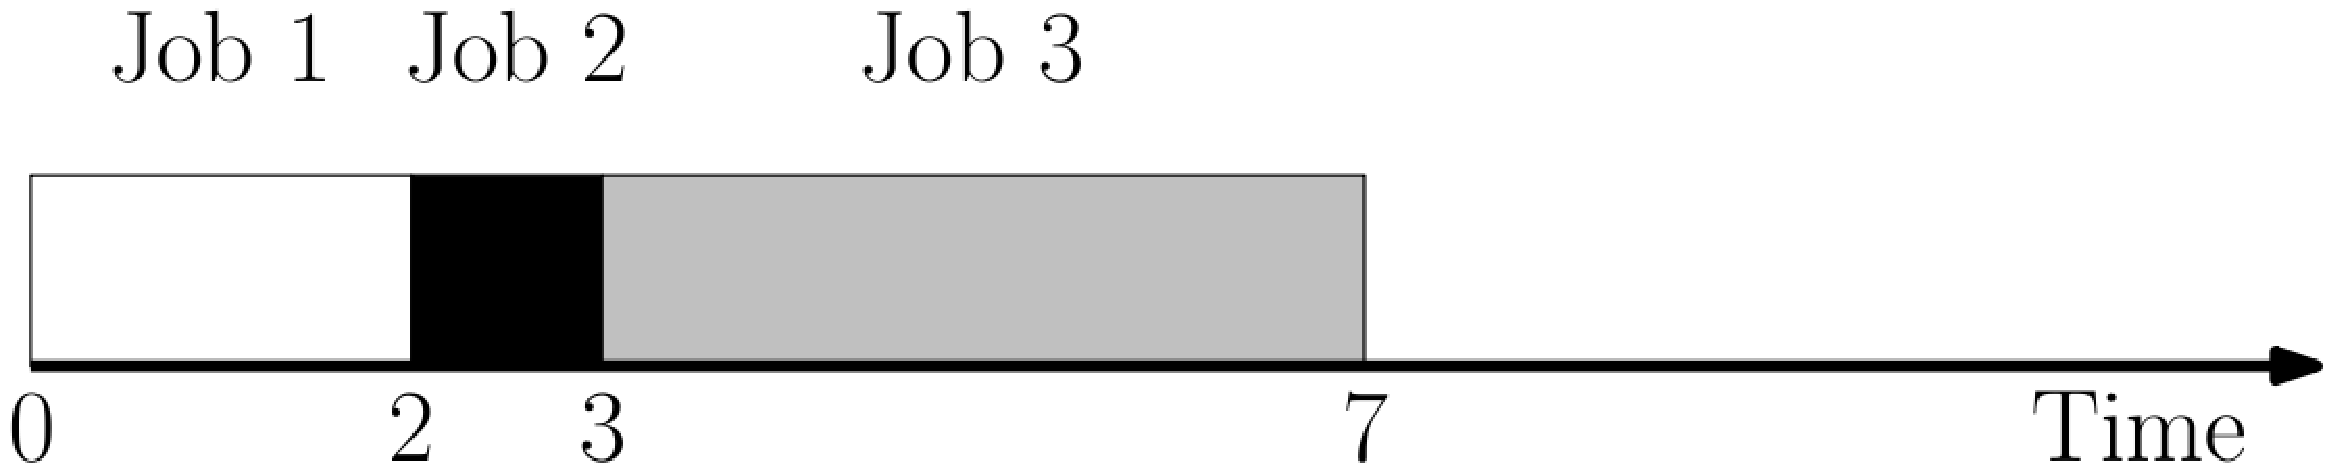
\includegraphics[scale=0.2]{ordo.pdf}
    \caption{Ordonnancement optimal \textit{(Job $1 = A$, Job $2 = B$,
    Job $3 = C$)}}
    \end{center}
\end{figure}
\noindent En effet, on a :
\begin{itemize}
\item $retard(A) = 2 - (-1) = 3$
\item $retard(B) = 3 - 1 = 2$
\item $retard(C) = 7 - 10 = -3$, dans ce cas-ci on est en avance.
\end{itemize}

$\hookrightarrow L_{MAX} = 3$ et on ne peut faire mieux, et ce, pour 2 raisons :
\begin{itemize}
\item C'est la tâche $A$ qui cause le retard maximum de $3$,
\item pour $A$, on ne peut pas faire mieux car on l'a faite le plus tôt
possible.
\end{itemize}

\noindent Ceci était un exemple, nous généralisons à présent le problème. En
général, on a :
\begin{itemize}
\item $n$ tâches,
\item chaque tache $j$ possède :
	\begin{itemize}
	\item[$\bigstar$]un \textbf{temps de complétion} : $p_j$,
	\item[$\bigstar$]une \textbf{release date} : $r_j$,
	\item[$\bigstar$]une \textbf{deadline} : $d_j$,
   \end{itemize}
\end{itemize}

\noindent Aussi, pour chaque solution réalisable, nous introduisons certaines
notations:
\begin{itemize}
\item $c_j$ $=$ instant ou $j$ est finie,
\item $L_j$ \textit{(lateness)} $= c_j - d_j$,
\item $L_{MAX}$ = $\max_{j}(L_j)$.
\end{itemize}

\begin{exemple}[Pour la même instance] On a :
\begin{itemize}
\item $p_1 = 2,\ r_1 = 0,\ d_1 = -1$
\item $p_2 = 1,\ r_1 = 2,\ d_1 = 1$
\item $p_3 = 4,\ r_1 = 1,\ d_1 = 10$
\end{itemize}
\indent $\quad$ Et pour l'ordonnancement \textbf{ABC}:
$L_{MAX} = L_1 = c_1 - d_1 = 2-(-1) = 3$
\end{exemple}

\begin{pblm}
\textbf{MIN Schedule Single-Machine(\titre{SSM})}
\begin{itemize}
\item[*]\textbf{\underline{Instance}} : $n$ jobs (triplets ($p_j$,$r_j$,$d_j$)),
\item[*]\textbf{\underline{Solution}} : schedule des $n$ jobs ($\simeq\ c_j$ et
$L_j$),
\item[*]\textbf{\underline{Mesure}} : $L_{MAX}$
\end{itemize}
\end{pblm}

\newpage

\noindent Pour simplifier, pour tout $j$, on émet les hypothèses suivantes :
\begin{enumerate}
\item[$\mathbf{Hyp_1}$ :] $r_j$ et $p_j \geq 0$
\item[$\mathbf{Hyp_2}$ :] $d_j < 0$ \textit{(pour être sur que $L_{MAX}$ soit
$> 0$, et pour simplifier les choses vu qu'une seule deadline dans le passé
suffirait)}
\end{enumerate}

\begin{rem}
Imaginons un algorithme de $f$-\textit{approximation} et que la solution
optimale est $=0$. Par la définition, on a $APP.f=OPT$, c'est-à-dire $0.f = 0$
ce qui est gênant par rapport à la définition\dots~alors
$\mathcal{P} = \mathcal{NP}$ ? \\
$\Rightarrow$ On suppose que l'optimal est toujours $> 0$.
\end{rem}

\begin{exemple}
$p_j$ et $r_j$ identiques que précédemment, on pose :
		  $$d'_j = d_j - (\max_j (d_j + 1))$$
$\rightarrow (\max_j (d_j + 1)) = 11$\\
$\rightarrow d'_1 = -12, d'_2 = -10, d'_3 = -1 \Rightarrow L'_{MAX} = L_{MAX} +
11 = 3+11 = 14$ \\
$\hookrightarrow$ on ne fait qu'une translation dans le temps, on peut retomber
sur l'instance initiale simplement en soustrayant l'écart utilisé.
\end{exemple}

Nous allons maintenant élaborer un premier algorithme permettant d'approcher la
solution optimale. Il s'agit d'un algorithme privilégiant la tâche de deadline
la plus proche ou en anglais \textit{``Earliest Due Date (\textbf{EDD})''}
$\rightarrow$ on commence par celle la plus en retard dans le cas où il y a des
deadlines négatives.

\begin{algorithm}[h!]
\caption{EDD\_SSM}
\begin{algorithmic}[1]
\STATE $t\leftarrow 0$
\STATE $todo \leftarrow \{1,2,\ldots,n\}$
\WHILE{$todo$ n'est pas vide}
\IF{au moins une tâche est disponible ($r_j \leq t$ ?)}
\STATE $j\leftarrow arg\min_j{d_j}$
\STATE $t\leftarrow t+p_j$ \textit{// le temps d'exécution est ajouté au temps
courant}
\STATE $c_j \leftarrow t$ \textit{// le temps à laquelle la tâche est terminée
est mis à jour}
\STATE $todo \leftarrow todo \setminus \{j\}$
\ELSE
\STATE $t\leftarrow \min_{j\in todo}(r_j)$ \textit{// On avance à la tâche la
plus rapidement disponible}
\ENDIF
\ENDWHILE
\STATE Calculer et retourner $L_{MAX}$
\end{algorithmic}
\end{algorithm}

Soit $S$ un sous-ensemble de tâches, on définit
\begin{itemize}
\item $r(S) = \min_{j\in S} r_j$ \textit{(la date de dispo au plus tôt pour S)}
\item $p(S) = \sum_{j\in S} p_j$ \textit{(temps pour tout accomplir sans
``trou'')}
\item $d(S) = \max_{j\in S} d_j$ \textit{(la deadline la + éloignée)}
\item $L^*_{MAX} = OPT$.
\end{itemize}
\newpage
\begin{lemme} Pour tout sous-ensemble de tâches $S$,
$$ L^*_{MAX} \geq r(S) + p(S) - d(S) $$
\begin{proof}
Soit un ordonnancement optimal pour toutes les tâches ($n$ tâches), voyons le
simplement comme un ordonnancement pour $S$.

\begin{exemple} (exemple précédent)
\begin{figure}[h!]
    \begin{center}
    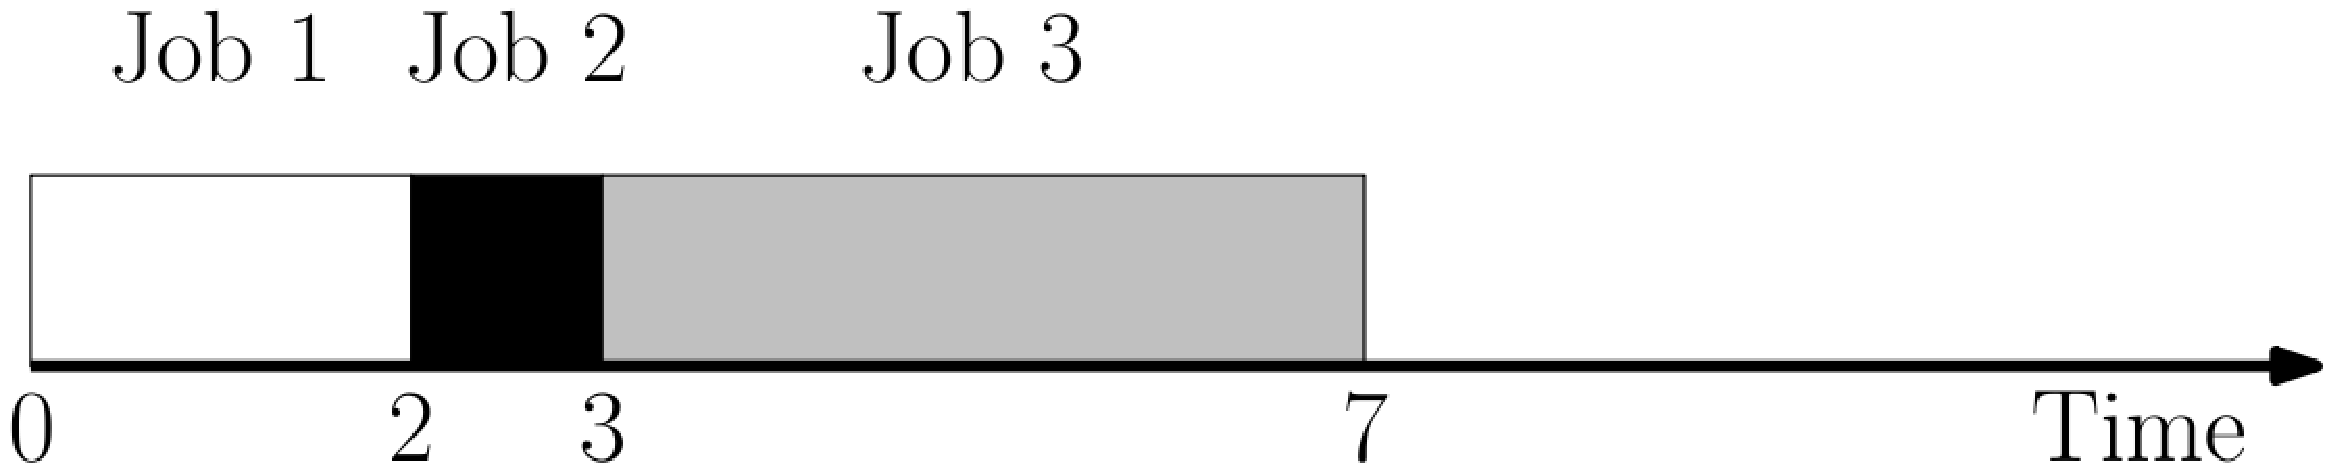
\includegraphics[scale=0.2]{ordo.pdf}
    \caption{Ordonnancement optimal \textit{(Job $1 = A$, Job $2 = B$,
    Job $3 = C$)}}
    \end{center}
\end{figure}

Si on prend $S = \{A,C\}$ :
\begin{figure}[h!]
    \begin{center}
    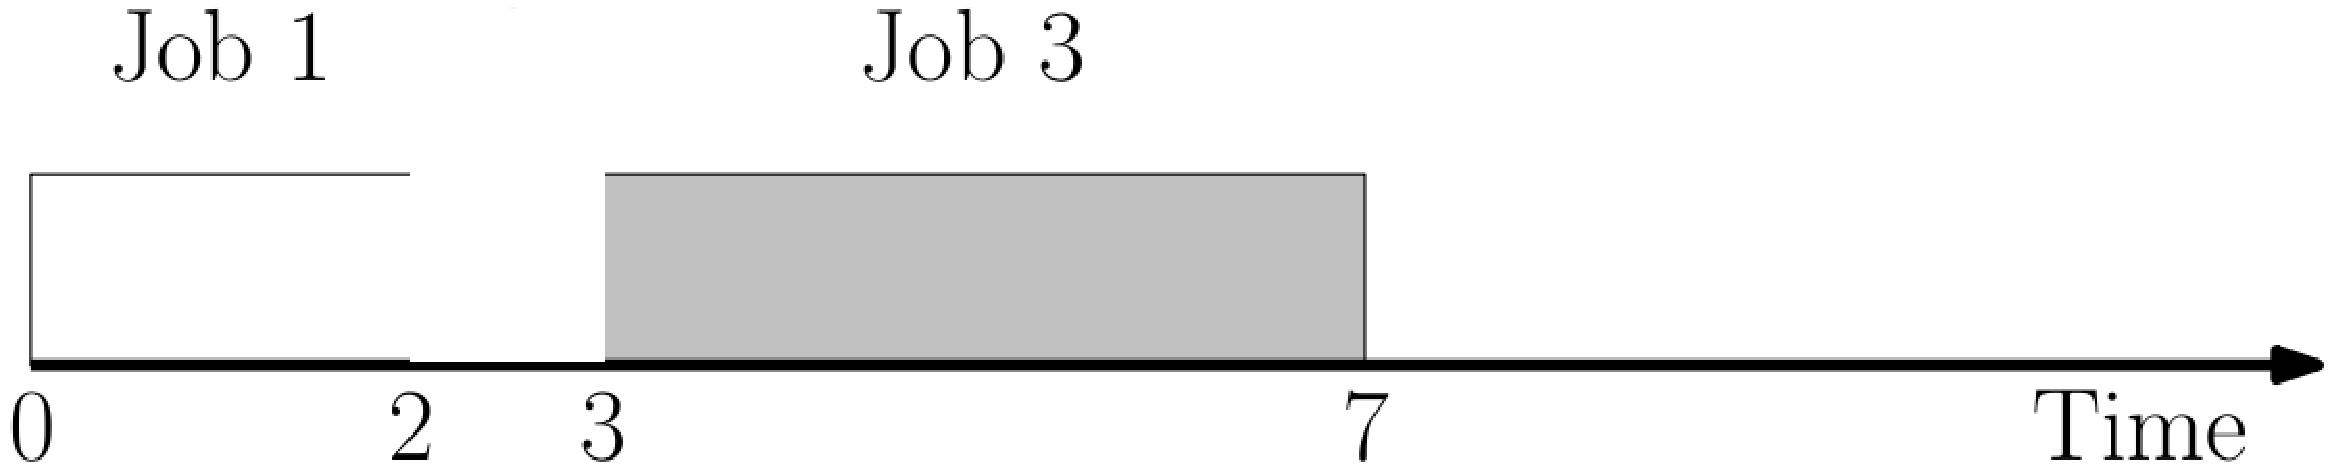
\includegraphics[scale=0.2]{ordoPart.pdf}
    \caption{Ordonnancement optimal concentré sur $S$ \textit{(Job $1 = A$,
    Job $3 = C$)}}
    \end{center}
\end{figure}
\end{exemple}
Soit $j$ la dernière tâche traitée dans $S$ :
\begin{itemize}
	\item[\textbf{(1)}] aucune tâche ne peut être exécutée avant $r(S)$,
	\item[\textbf{(2)}] au total on a besoin de minimum $p(s)$ unité de temps.
	\item[$\rightarrow$] de \textbf{(1)} et \textbf{(2)} on tire que $j$ ne peut
    pas être finie avant $r(S)+p(S)$,
  	\item[$\rightarrow$] on sait également, par définition de $d(S)$, que
    $d(j) < d(S)$.
  	\item[$\rightarrow$] le retard pour la tâche $j$ est au moins
    $r(S)+p(S) - d(S)$
  	\item[$\hookrightarrow$] $L^*_{MAX} \geq r(S)+p(S)-d(S)$ (vu que
    $L^*_{MAX}$ est le retard maximal)
 \end{itemize}
 \cqfd
\end{proof}
\end{lemme}

\begin{thm}[EDD\_SSM est un algorithme de 2-approximation pour le problème SSM]
(si les hypothèses $\mathbf{Hyp_1}$ et $\mathbf{Hyp_2}$ sont vérifiées)
\begin{proof}
Soit l'ordonnancement donné par \textbf{EDD\_SSM} et soit $j$ la tâche ayant le
plus grand retard, on a donc : $$L_{MAX} = c_j - d_j\qquad\qquad
\text{\textbf{(1)}}$$ Faisons un focus sur $c_j$, soit $t \leq c_j$ l'instant le
plus tôt tel que la machine est utilisée sans interruption pour toute la
période $[t,c_j[$, c'est-à-dire la situation suivante :

\begin{figure}[h!]
    \begin{center}
    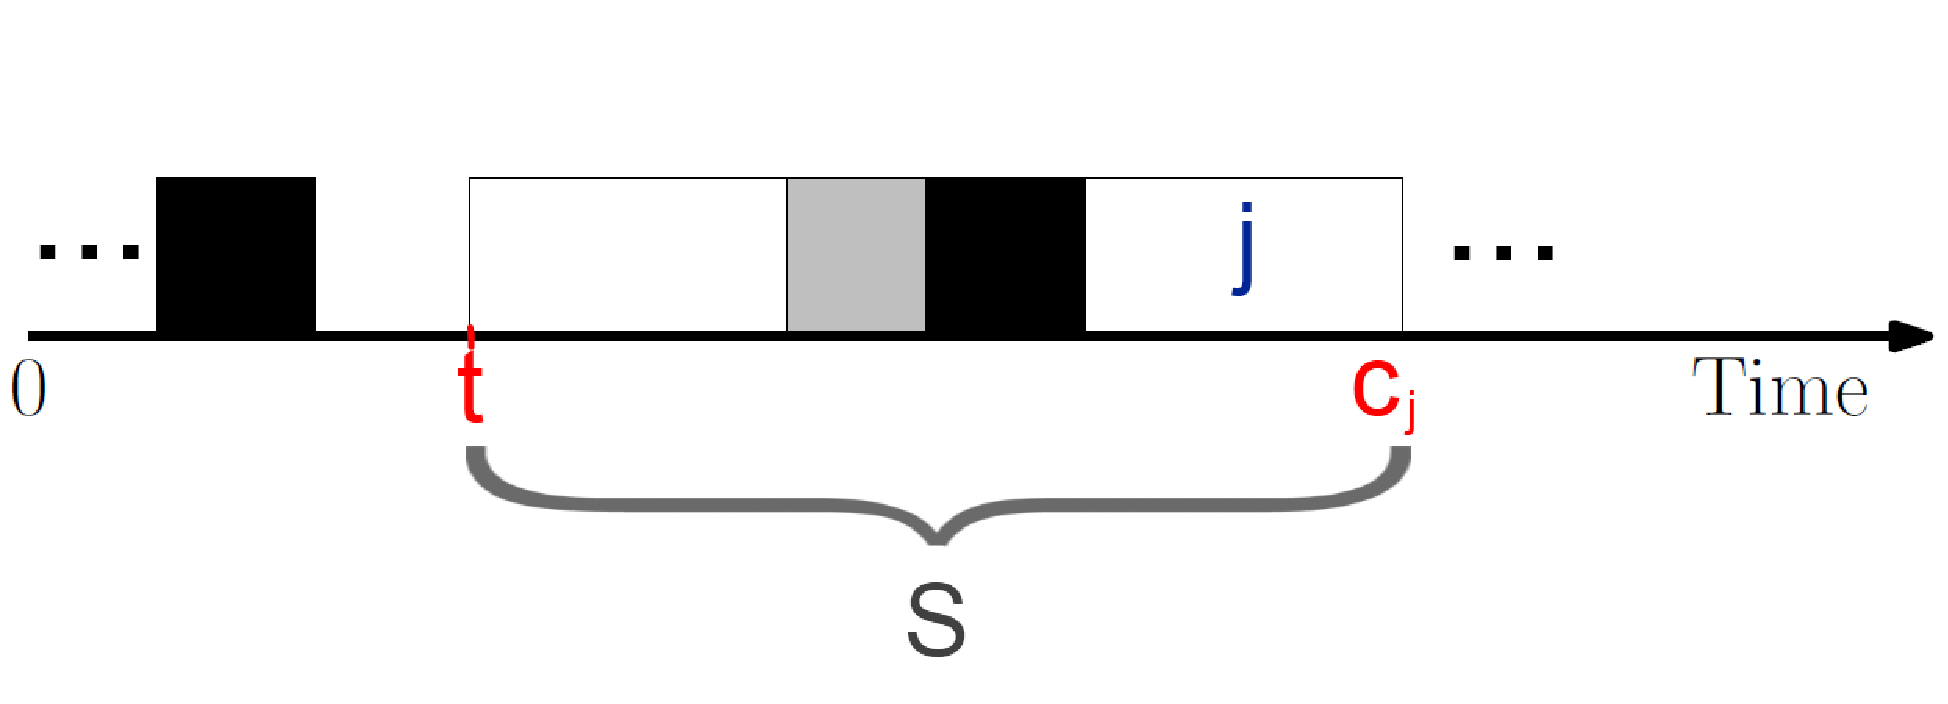
\includegraphics[scale=0.25]{ssm.pdf}
    \caption{Exemple général}
    \end{center}
\end{figure}
\newpage
\noindent Sur l'intervalle $[t,c_j[$ et $S$ on sait :
\begin{itemize}
\item[$\bigstar$] $r(S) = t$, en effet, juste avant $t$ il y a un repos
(par définition), donc aucune tâche de $S$ n'était disponible avant $t$ (et donc
tous les $r_j$ de $S$ sont $\geq t$ (au moins une est égale à $t$, par
définition de $t$ toujours).
\item[$\bigstar$] $p(S) = c_j - t$ (vu qu'il n'y a pas de pause par
construction) $= c_j - r(S)$
$$\Longrightarrow c_j = r(S)+p(S) \qquad\qquad \text{\textbf{(2)}}$$
\end{itemize}
Comme $d(S) < 0$ \textit{(par les hypothèses faites précédemment)}, par le
lemme, on a $$L^*_{MAX} \geq r(S) + p(S) - d(S) \geq r(S)+p(S) = c_j\
\text{\textit{par (2)}}\qquad\qquad \text{\textbf{(3)}}$$

Si on applique à nouveau le lemme avec $S = \{j\}$, on a :
$$L^*_{MAX} \geq r_j + p_j - d_j \geq -d_j\qquad\qquad \text{\textbf{(4)}}$$

En combinant (3) et (4) (en sommant les 2 cotés) on a :
$$L_{MAX} =_{(1)} c_j - d_j \leq 2L^*_{MAX}\qquad\qquad
\text{\textit{(par (3) et (4))}}$$

et donc $$\frac{L_{MAX}}{L^*_{MAX}} \leq 2$$
\cqfd
\end{proof}
\end{thm}

\subsection{Le problème ``$k$-\textit{centre}''}

La motivation de ce problème est de faire du clustering, c'est-à-dire diviser
un ensemble de données en plusieurs sous-groupes contenant des données
``proches'' au sens d'une certaine distance à définir. Dans notre cas nous
utiliserons la distance euclidienne.

\begin{pblm}
\textbf{MIN $k$-centre}
\begin{itemize}
\item[*]\textbf{\underline{Instance}} :
\begin{itemize}
\item graphe non-dirigé complet $G = (V,E)$ pondéré avec une distance $d_{ij}
\geq 0$ entre toute paire $i$, $j$ de sommets (on a donc
une matrice des distances),
\item un entier $k$ ;
\end{itemize}
\item[*]\textbf{\underline{Solution}} : $S\subseteq V$ tel que $|S|=k$,
sous-ensemble d'éléments appelés les centres.
\item[*]\textbf{\underline{Mesure}} : distance maximum entre un sommet et son
centre (le plus proche), cette distance est appelée le rayon.
\end{itemize}
\end{pblm}

On fait l'hypothèse que la distance utilisée est bien une distance au sens
mathématique, c'est-à-dire qu'elle réunit les 3 propriétés :
\begin{itemize}
\item $\forall i \in V,\ d_{ii} = 0$
\item $\forall i,j\in V,\ d_{ij}=d_{ji}$
\item $\forall i,j,k \in V,\ d_{ij} \leq d_{ik} + d_{kj} \qquad$
\textit{(inégalité triangulaire)}
\end{itemize}

\newpage

\begin{exemple}$ $\\

\begin{figure}[h!]
    \begin{center}
    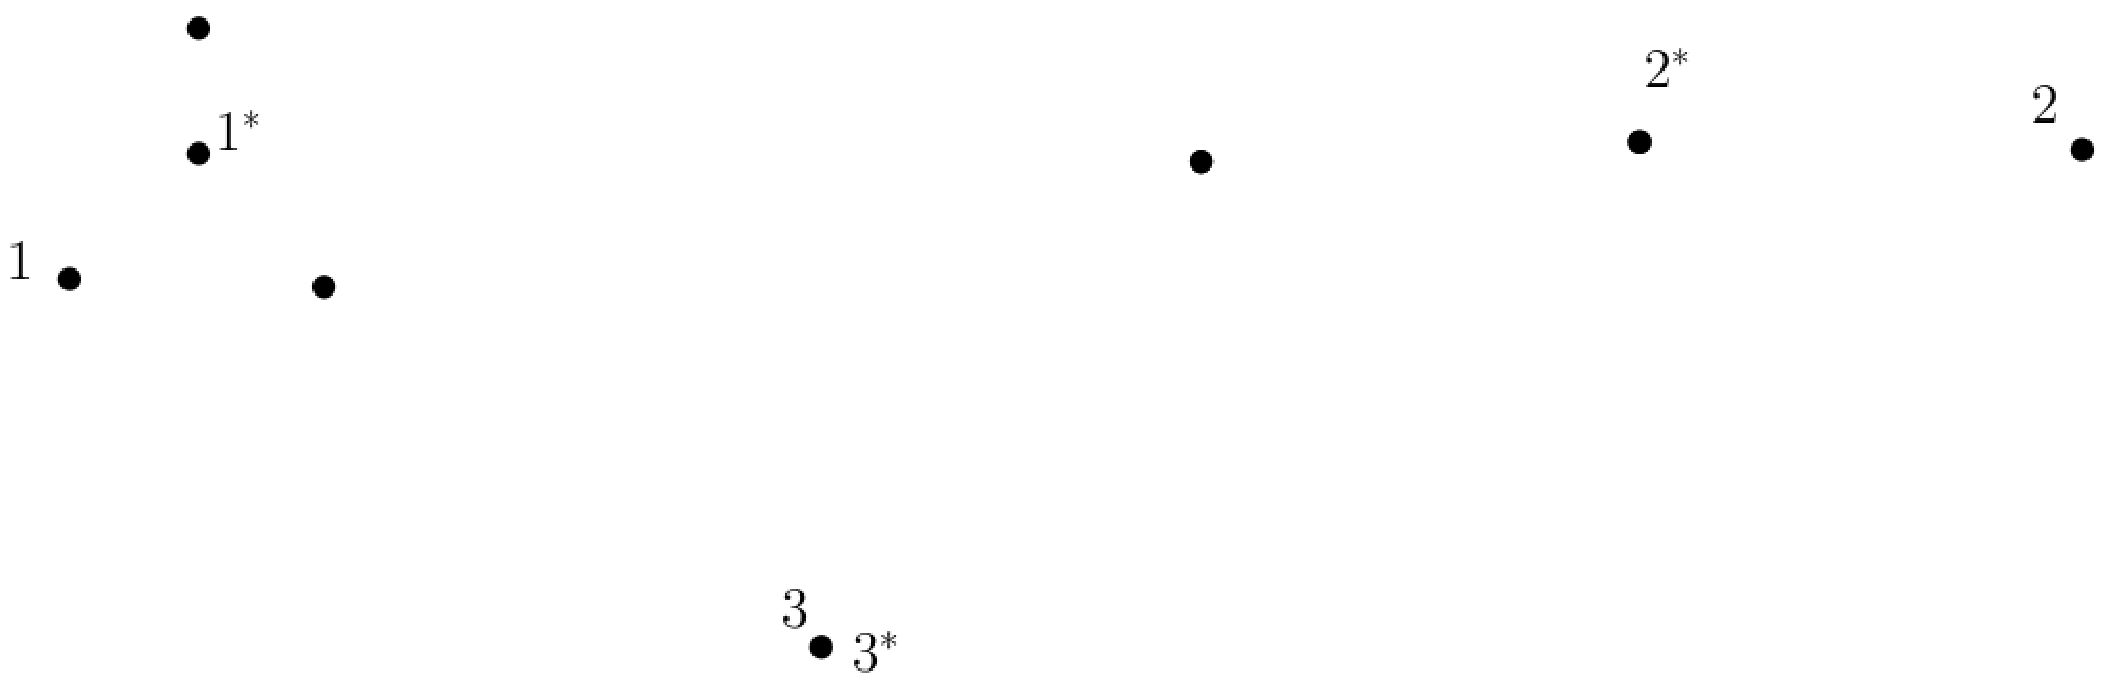
\includegraphics[width=0.6\textwidth]{inst_kcentre.pdf}
    \caption{Exemple de solution optimale d'une instance avec $k=3$}
    \end{center}
\end{figure}
\textit{(les nombres avec une étoile sont ceux représentant les centres des
groupes)}\\
Dans cet exemple, la distance maximale (le rayon), et donc la mesure de cette
solution, est la distance entre le point $2$ et le point $2^*$.
\end{exemple}

Nous allons à présent essayer d'élaborer un algorithme glouton permettant de
définir au moins les bons groupes, même s'il ne trouve pas forcément le bon
point comme centre de chaque groupe. Nous proposons de commencer l'algorithme
par sélectionner un point au hasard comme centre puis on va itérer en prenant
à chaque fois le point le plus loin des centres déjà sélectionné. Pour ce faire,
nous introduisons une notation : soit $S$ l'ensembles des centres, on note
$d(i,S) = \min_{j\in S}(d_{ij})$, on a donc : $$rayon = \max_{i\in V} d(i,S)$$

\begin{algorithm}[h!]
\caption{Greedy\_k\_center}
\begin{algorithmic}[1]
\STATE Choisir $i\in V$ au hasard.
\STATE $S\leftarrow \{i\}$
\WHILE{$|S| < k$}
\STATE $j\leftarrow arg\max_{j\in V}d(j,S)$
\STATE $S\leftarrow S \cup \{j\}$
\ENDWHILE
\end{algorithmic}
\end{algorithm}

Quel est le pire des cas pour cet algorithme ? Voici un exemple serré
(``tight'') du pire des cas (ce qui signifie qu'il montre que le
facteur d'approximation est atteint).

\setlength{\unitlength}{1.0cm}
\begin{exemple}$ $\\
\begin{picture}(10,4)(0,0)
% CLUSTER 1
\put(2,2){\circle*{0.1}}
\put(3,2){\color{red} \circle*{0.1}}
\put(4,2){\circle*{0.1}}
\put(3,3){\circle*{0.1}}
% CLUSTER 2
\put(8,3){\circle*{0.1}}
\put(9,2.5){\circle*{0.1}}
\put(10,3){\color{red} \circle*{0.1}}
% CLUSTER 3
\put(6,0){\color{red} \circle*{0.1}}
\end{picture}

Sur le dessin \textit{(les centres sont en rouges)} on a:
$$d_{ab} = 2 d_{ac} = 2 d_{bc} $$

Dans ce cas, on fait $2$ fois moins bien. L'algorithme peut donc faire
\textbf{au moins} $2$ fois pire\\
\indent (et en fait $2$ est le facteur d'approximation).
\end{exemple}

\newpage

\begin{thm} \textbf{Greedy\_$k$\_center} est un algorithme de $2$-approximation
pour le problème \textbf{$k$-center}.
\begin{proof}$ $\\
\begin{itemize}
\item \textbf{L'algorithme s'effectue-t-il en temps polynomial ?}
$\hookrightarrow$ oui, de manière triviale.
\item \textbf{L'algorithme a-t-il un facteur d'approximation égal à 2 ?} \\
Soit $S^* = \{j_1,\ldots ,j_k\}$ une solution optimale et $r^*$ le rayon de
$S^*$.\\
$\Rightarrow$ cette solution partitionne $V$ en groupes $V_1,...,V_k$ où chaque
sommet $j\in V$ est placé dans un groupe $V_i$ s'il est le plus proche du centre
$j_i$ parmi tous les centres $S^*$ (égalités brisées arbitrairement). \\
\begin{center}
	\textbf{Fait (1)} : chaque paire de points $j,j'$ dans un même groupe $V_i$
    est telle que $d_{jj'} \leq 2r^*$.\\
\end{center}

Ce fait est logique vu que $r^*$ est le rayon du plus gros cluster, les 2 points
les plus éloignés possibles sont donc de part et d'autres  du centre de ce
cluster à une distance exacte de $r^*$.
\begin{enumerate}
\item Supposons d'abord que chaque centre de $S$ est sélectionné par
l'algorithme parmi chacun des groupes $V_1,\ldots V_k$ déterminés par $S^*$.
Par le \textbf{fait (1)}, tout sommet de $V$ est à distance $\leq 2r^*$ d'un des
centres de $S$ $\Rightarrow$ le théorème est prouvé.
\item Supposons maintenant que ce ne soit pas le cas, c'est-à-dire que
l'algorithme sélectionne $2$ points dans le même groupe $V_i$.
Cela veut dire que lors d'une certaine itération $j\in V_i$ est choisi alors
que $j'\in V_i$ avait déjà été choisi. Par le \textbf{fait (1)}, on sait que
$$d_{jj'} \leq 2r^*$$
Or l'algorithme choisit $j$ car il est actuellement \textbf{le point le plus
éloigné} des centres contenus dans $S$ à cette itération.
Donc, tous les points sont à distances $\leq 2r^*$ d'un des centres déjà dans
$S$. Cette observation reste vraie à la fin de l'algorithme (le fait d'ajouter
des centres dans $S$ n'augmente pas la distance maximale).
\end{enumerate}
\end{itemize}
\cqfd
\end{proof}
\end{thm}

Nous allons maintenant prouver qu'il n'est pas possible de faire mieux comme garantie théorique. En effet, il existe des heuristiques
effectuant des meilleurs choix que notre algorithme glouton mais elles n'ont pas de meilleure garantie théorique que ce facteur $2$. Ceci
signifie que, même si elles donnent de meilleurs résultats en moyenne, il existe des instances pour lesquelles elles fourniront une
solution équivalente à $2$ fois la solution optimale. \\
Afin d'effectuer cette preuve, nous allons nous ramener à un problème de décision connu pour être $\mathcal{NP}$-difficile, le problème
du \textbf{Dominating Set}.

\begin{pblm}
\textbf{Dominating Set (decision) (\titre{DS})}
\begin{itemize}
\item[*]\textbf{\underline{Instance}} :
\begin{itemize}
\item Graphe $G=(V,E)$,
\item entier positif $k$;
\end{itemize}
\item[*]\textbf{\underline{Question}} : Existe-t-il un ensemble $S\subseteq V$ de taille $k$ tel que chaque sommet de $V$ est soit dans
$S$ soit adjacent à un sommet de $S$ ?
\end{itemize}
\end{pblm}

\newpage

\begin{exemple}$ $\\

\begin{figure}[h!]
    \begin{center}
    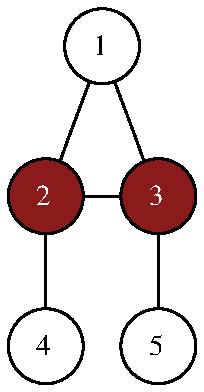
\includegraphics[scale=0.5]{inst_ds.pdf}
    \caption{Exemple d'instance du \textbf{\titre{DS}}}
    \end{center}
\end{figure}
\noindent Si $k=1 \Rightarrow$ \textbf{NO} \\
Si $k=2 \Rightarrow$ \textbf{YES} \textit{(en prenant l'ensemble $S=\{2,3\}$)}
\end{exemple}

Comment peut-on transformer une instance de \textbf{\titre{DS}} en une instance de $k$-center ? Pour le graphe, rien de bien particulier,
la notion importante à définir ici est la distance à utiliser, prenons :
\begin{itemize}
\item $d_{ij} = 1$ si $(i,j) \in E$
\item $d_{ij} = 2$ sinon \\
\end{itemize}

En imaginant qu'il existe un algorithme d'approximation de facteur $f < 2$ pour résoudre \textbf{$k$-center}, alors si la réponse est $2$
pour cet algorithme cela veut dire que la réponse est \textbf{NO} pour le \textbf{\titre{DS}}. On aurait alors là un algorithme
polynomial capable de résoudre un problème $\mathcal{NP}$-difficile de manière exacte$\ldots$ ce qui signifierait que $\mathcal{P=NP}$ !
On peut utiliser cet argument pour prouver qu'on ne peut faire mieux qu'un facteur $2$ pour résoudre \textbf{$k$-center}.

\begin{thm}Il n'y a pas d'algorithme d'$\alpha$-approximation pour le \textbf{$k$-center} avec $\alpha <2$.\\ (à moins que $\mathcal{P} =
\mathcal{NP}$)
\begin{proof}$ $\\
Soit $A$ un algorithme d'approximation de facteur $<2$, montrons qu'on peut utiliser $A$ pour résoudre \textbf{\titre{DS}} en temps
polynomial. A partir d'une instance $(G,k)$ du \textbf{\titre{DS}}, on définit une instance pour le \textbf{$k$-center} comme suit :
\begin{itemize}
\item [$\bigstar$]$d_ij = 1$ si $(i,j) \in E$
\item [$\bigstar$]$d_ij = 2$ sinon.
\end{itemize}
$\Rightarrow$ il y a un ensemble dominant de taille $k$ ssi le rayon optimal est $1$ pour le \textbf{$k$-center}.\\
$\Rightarrow$ comme l'algorithme $A$ possède un facteur $< 2$, la mesure du problème du $k$-center doit obligatoirement trouver une
solution ayant un rayon égal à 1 si une telle solution existe \textit{(car la solution est un entier)}.
\cqfd
\end{proof}
\end{thm}

\newpage

\subsection{Ordonnancement de tâches sur des machines identiques parallèles}

\begin{flushright}\textit{(un des deux premiers algorithmes d'approximation : années 60)}\end{flushright}

Il s'agit d'une variation du \textbf{\titre{SSM}} :
\begin{itemize}
\item il y a maintenant plusieurs machines,
\item pas de \textit{release date} ni de \textit{deadline},
\item but : minimiser le temps utilisé pour terminer toutes les tâches.
\end{itemize}

\begin{pblm}
\textbf{MIN Schedule Parralel Machine (\titre{SPM})}
\begin{itemize}
\item[*]\textbf{\underline{Instance}} :
\begin{itemize}
\item entiers $m$ (machines) et $n$ (tâches),
\item pour chaque tâche $j$, un temps de complétion $p_j$ (unités de temps sans
interruption).
\end{itemize}
\item[*]\textbf{\underline{Solution}} : Scheduling des $n$ tâches sur les $m$
machines.
\item[*]\textbf{\underline{Mesure}} : $c_{MAX} = \max_j c_j$
\end{itemize}
\end{pblm}

\subsubsection{Approche par la recherche locale}

\begin{exemple}[$m=5$ et $n=10$]$ $\\
\begin{figure}[h!]
    \begin{center}
    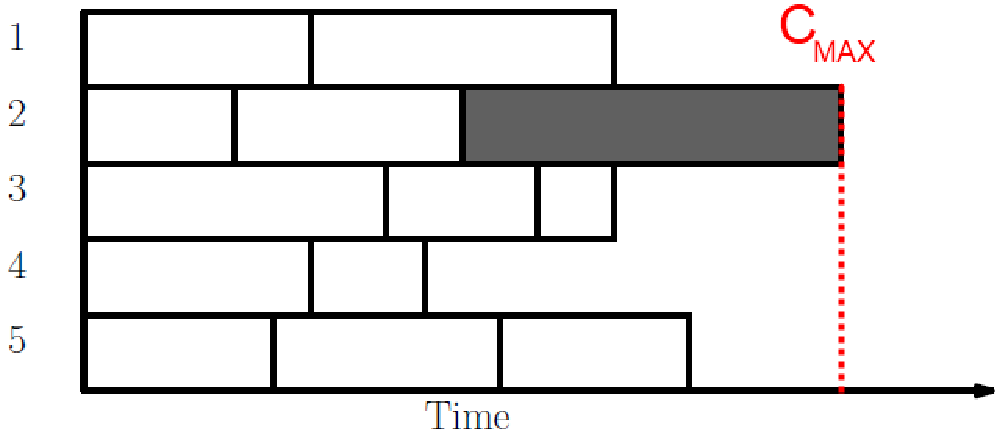
\includegraphics[scale=0.5]{spm1.pdf}
    \caption{Exemple de solution d'une instance du \textbf{\titre{SPM}}}
    \end{center}
\end{figure}

Via un algorithme de recherche locale que l'on appellera \textbf{LocalSearch\_SPM}, on pourrait choisir comme voisinage par exemple le
fait de prendre la tâche qui se finit le plus tard pour la mettre sur la machine qui n'est plus utilisé le plus tôt. On va même
simplifier en déplaçant la tâche vers une machine permettant de diminuer $C_{MAX}$. Imaginons que cette tâche est la tâche $l$, on va la
déplacer vers une machine qui se termine avant $c_l-p_l$. Appliquons l'algorithme (une seule itération) :

\begin{figure}[h!]
    \begin{center}
    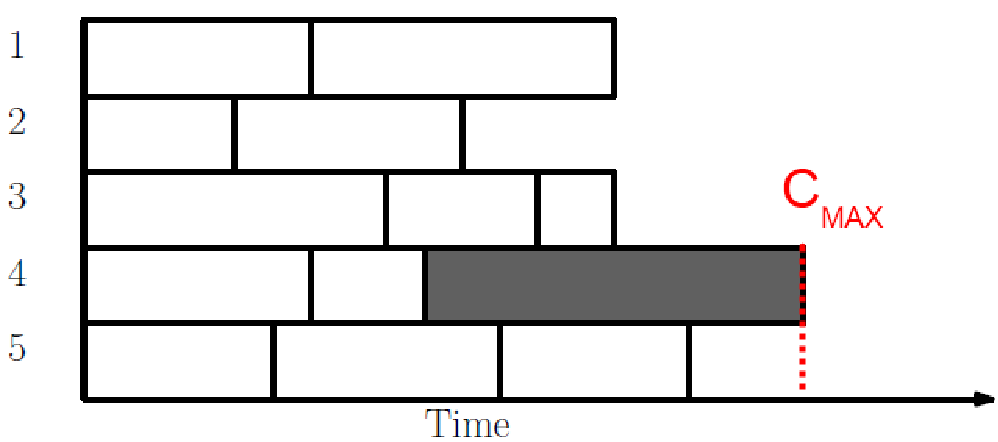
\includegraphics[scale=0.5]{spm2.pdf}
    \caption{Exemple de solution d'une instance du \textbf{\titre{SPM}}}
    \end{center}
\end{figure}

$\Longrightarrow$ \textbf{Optimum local.}
\end{exemple}

\newpage

Notons $c^*_{MAX}$ la longueur d'un schedule optimal, on peut alors dire que ce schedule prendra au moins le temps d'exécution de la plus
longue des tâches soumises :
$$\boxed{c^*_{MAX} \geq \max_{j=1,\ldots,n} p_j} \qquad\qquad \text{\textbf{(1)}}$$
D'autre part, il y a au total un temps de travail $P = \sum_{j=1}^n p_j$ et $m$ machines ; donc en
moyenne une machine travaille $\frac{P}{m}$ unité de temps. Il y a donc au moins
une machine qui travaille pendant un temps $t \geq \frac{P}{m}$ (sinon la moyenne n'est pas la moyenne $\ldots$ !) et donc :
$$\boxed{c^*_{MAX} \geq \frac{P}{m} = \frac{\sum_{j=1}^n p_j}{m}} \qquad\qquad \text{\textbf{(2)}}$$

Prouvons à présent que l'algorithme que nous avons montré sur l'exemple plus haut est bien un algorithme d'approximation.

\begin{thm}L'algorithme LocalSearch\_SPM est un algorithme de $2$-approximation pour le problème \textbf{\titre{SPM}}.
\begin{proof}$ $\\
\begin{enumerate}
\item \textbf{L'algorithme s'exécute-t-il en temps polynomial ?}\\ (Voir preuve plus formelle dans livre de référence, chapitre 2) \\
$\hookrightarrow$ Intuitivement : l'algorithme est polynomial car le nombre d'itérations est borné par une fonction polynomiale.

\begin{figure}[h!]
    \begin{center}
    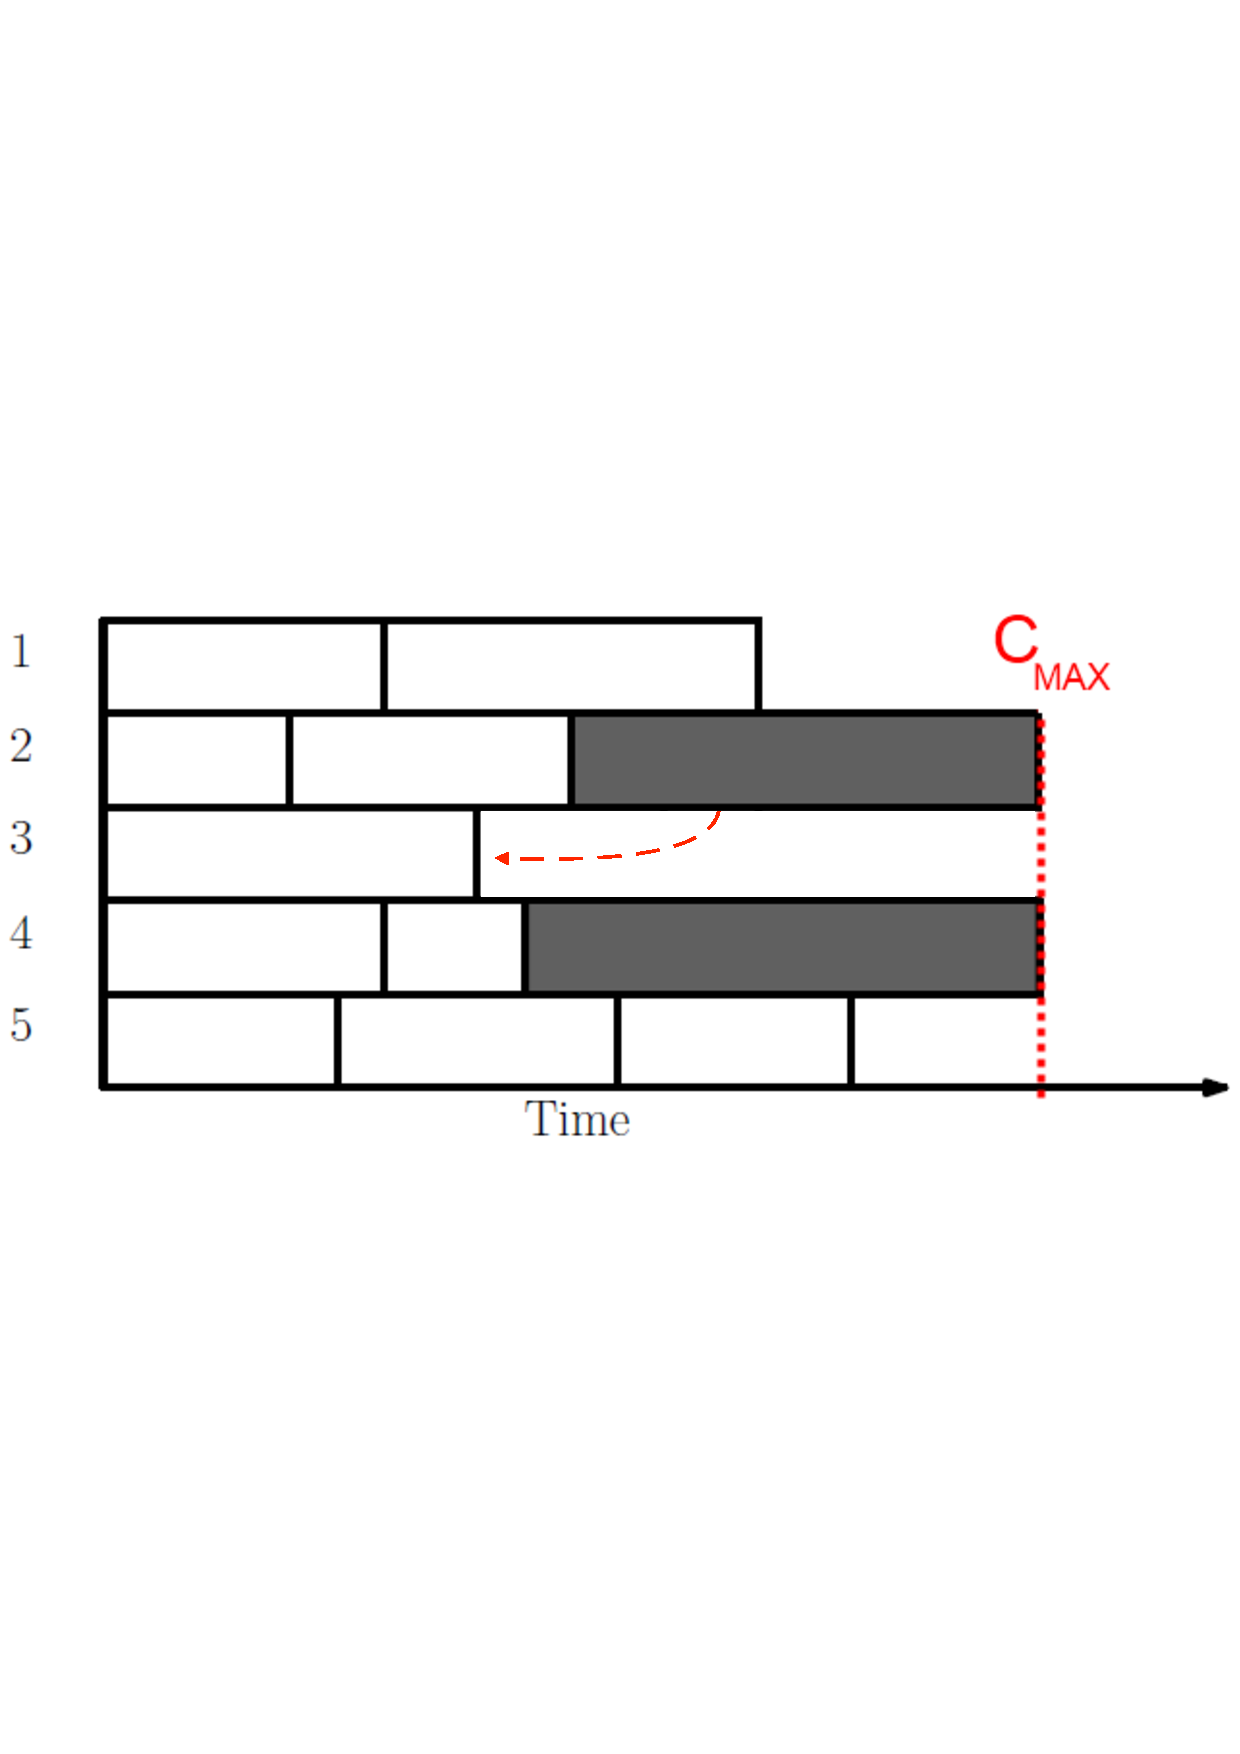
\includegraphics[scale=0.5]{spm3.pdf}
    \caption{Exemple où 2 machines atteignent $c_{MAX}$}
    \end{center}
\end{figure}

A chaque itération on va soit réduire $c_{MAX}$, soit diminuer le nombre de machines atteignant $c_{MAX}$ \\ $\Rightarrow$ nombre limité
d'étapes.\\

\item \textbf{L'algorithme possède-t-il un facteur d'approximation égal à 2 ?}\\
Soit une solution produite par \textbf{LocalSearch\_SPM}, soit $l$ la tâche se terminant en dernière, càd que $c_l = c_{MAX}$. On est
donc dans un cas comme suit (l'algorithme est terminé) :

\begin{figure}[h!]
    \begin{center}
    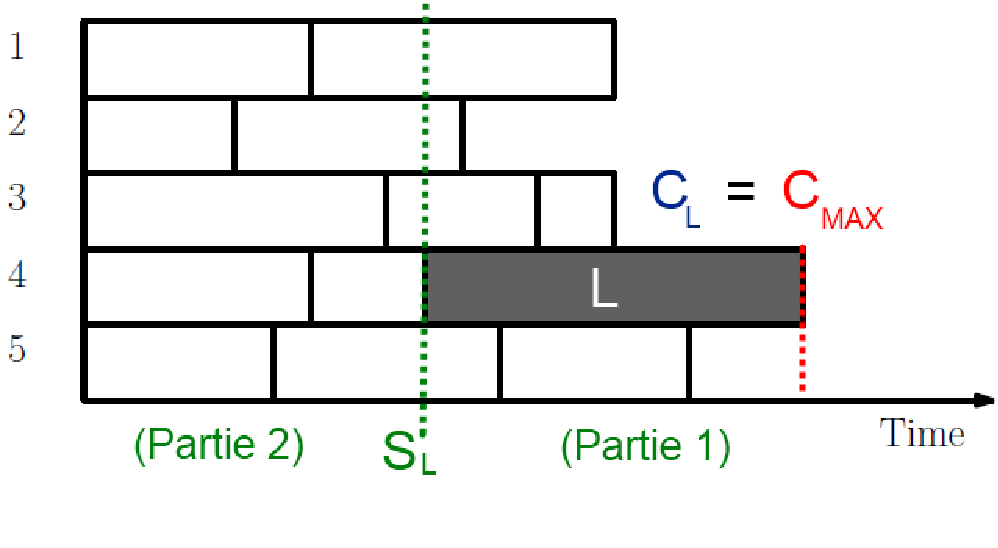
\includegraphics[scale=0.45]{spm4.pdf}
    \caption{Exemple de solution donnée par l'algorithme}
    \end{center}
\end{figure}

\newpage
Par le fait que l'algorithme est terminé, \textbf{toutes les machines sont au travail entre le temps $0$ et le début de la tâche $l$},
c'est-à-dire jusqu'en $S_l = c_l-p_l$.

\begin{itemize}
\item Le temps pris dans la \textit{(partie 1)} est égal à $p_l$ et par \textbf{(1)} ce temps est $\leq c^*_{MAX}$.
\item Le temps pris dans la \textit{(partie 2)} est égale à $m.S_l$ car toutes les machines sont au travail. Et on sait que $m.S_l \leq
P$ \textit{(plus petit que le travail total)} et donc $$S_l \leq \frac{P}{m} \leq c^*_{MAX} \qquad\qquad \text{\textit{(par
\textbf{(2)})}}$$
\end{itemize}
On conclut en observant que la fin du schedule se situe en $c_{MAX} \leq 2.c^*_{MAX}$ (en sommant les 2 parties du schedule qui sont
majorées par $c^*_{MAX}$).
\end{enumerate}
\cqfd
\end{proof}
\end{thm}

\subsubsection{Approche gloutone}

L'idée dans cette approche gloutone est de considérer les tâches dans un certain ordre et de les ajouter au schedule les unes à la suite
des autres. On peut alors imaginer trier les tâches dans un ordre aléatoire soit par ordre décroissant des $p_i$ et donc de considérer
d'abord les plus grandes et garder les plus petites pour la fin.

\begin{exemple}$m=2$ et $n=3$
$p_1 = 2$, $p_2 = 3$ et $p_3=4$

Si on les place selon l'ordre dans lequel les tâches sont données \textit{(``ListScheduling'')}, on obtient :

\begin{figure}[h!]
    \begin{center}
    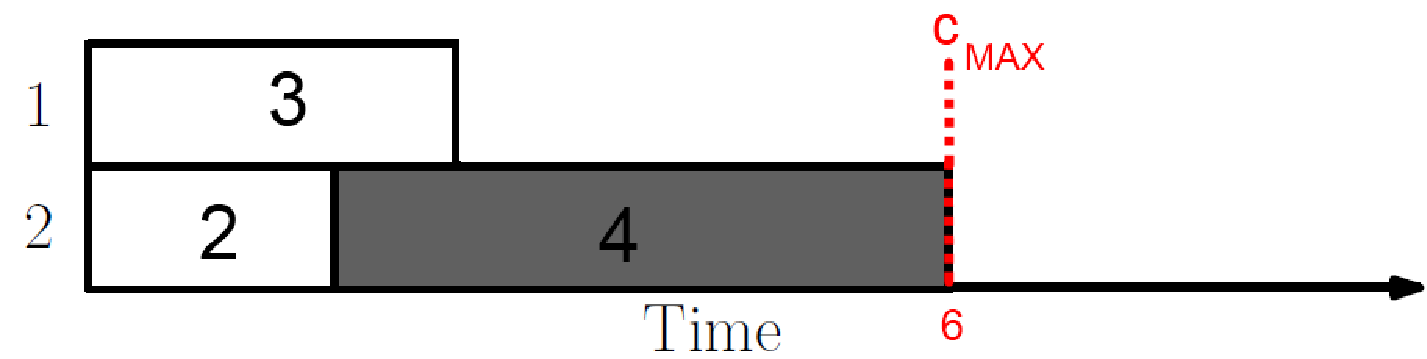
\includegraphics[scale=0.3]{spm5.pdf}
    \caption{Résultat du ListScheduling}
    \end{center}
\end{figure}

On remarque rapidement que cela dépend de l'ordre dans lequel on donne les tâches.  \\ Par exemple, l'ordre $3$, $1$, $2$ donne la solution
optimale :

\begin{figure}[h!]
    \begin{center}
    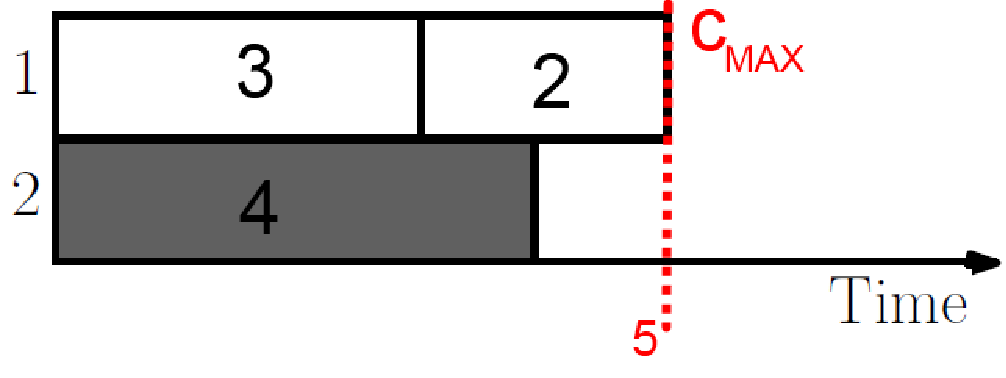
\includegraphics[scale=0.3]{spm6.pdf}
    \caption{Résultat du ListScheduling avec l'ordre $3$, $1$, $2$}
    \end{center}
\end{figure}

\end{exemple}

\begin{algorithm}[h!]
\caption{ListScheduling}
\begin{algorithmic}[1]
\STATE $todo$ $\leftarrow$ liste des tâches (liste = séquence ordonnée)
\FOR{chaque tâche $t$ dans todo}
\STATE Attribuer $t$ à une machine dont le temps de complétion est minimum
\ENDFOR
\end{algorithmic}
\end{algorithm}

De cet algorithme on pourrait tirer un algorithme naïf exact pour ce problème, il suffirait d'énumérer chaque permutation (ordre) possible
pour la liste et appliquer \textbf{ListScheduling} pour chacune de ces permutations et prendre celle qui donne la valeur la plus petite. Le
problème est que cet algorithme a une complexité factorielle (si liste de $n$ éléments, $n!$ permutations).

\newpage

\begin{thm} L'algorithme \textbf{ListScheduling} est un algorithme de $2$-approximation pour \textbf{\titre{SPM}}.
\begin{proof}$ $\\
Soit une solution donnée par l'algorithme \textbf{ListScheduling}, notons $l$ la tâche qui termine ce scheduling, càd $$c_l = c_{MAX}$$

\begin{figure}[h!]
    \begin{center}
    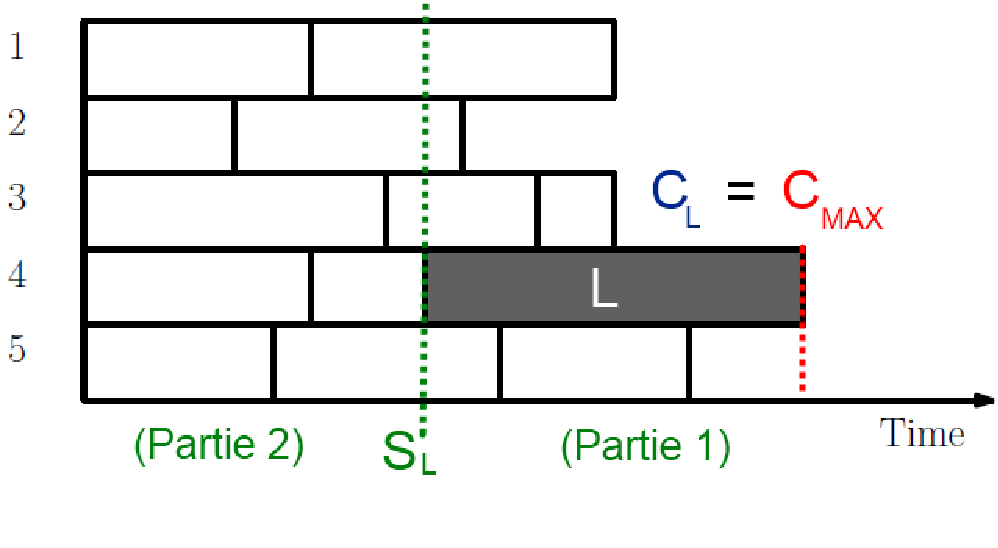
\includegraphics[scale=0.45]{spm4.pdf}
    \caption{Exemple de solution donné par l'algorithme}
    \end{center}
\end{figure}

\noindent (Exactement le même cas que pour LocalSearch vu que l'on place $l$ dans la
machine dont le temps de complétion est minimum, donc on aura jamais une tâche
$l$ que l'on pourrait placer plus tôt dans le scheduling courant)

\noindent \begin{itemize}
\item[$\Rightarrow$] Chaque machine est en activité jusque $S_l$, sinon on aurait pu
attribuer $l$ à une autre machine.
\item[$\Rightarrow$] Et donc, cela signifie que si on utilise \textbf{ListScheduling} pour la
solution initiale du \textbf{LocalSearch\_SPM}, ce dernier n'appliquera aucune itération car il se trouvera dans un optimum local. \\
\end{itemize}

\noindent Le facteur d'approximation $2$ est donc valable ici aussi (car on a finalement utilisé que l'algorithme glouton
\textbf{ListScheduling} dans cette ``recherche locale'').
\cqfd
\end{proof}
\end{thm}

\noindent A présent, nous allons considérer que :
\begin{itemize}
\item la liste est triée par ordre décroissant de $p_j$ $\Longrightarrow$ $p_1\geq p_2 \geq \ldots \geq p_n$
\item $n > m$ (car sinon $n\leq m$ et tout ordre est optimal vu que \textbf{ListScheduling} \\\indent $\qquad\quad$ va placer exactement
une tâche par machine) \\
\end{itemize}

Cette approche s'appelle \textbf{LPT} \textit{(Longest Processing Time rule)}, l'idée de manière formelle est :
\begin{itemize}
\item trier les tâches par ordre décroissant de $p_j$ $\Longrightarrow$ \textbf{polynomial},
\item appliquer \textbf{ListScheduling} sur ces tâches $\Longrightarrow$ \textbf{polynomial}.
\end{itemize}

\begin{exemple} Appliquons l'algorithme \textbf{LPT} sur l'exemple précédent.\\
$\Rightarrow p_1 = 4$, $p_2 = 3$, $p_3 = 2$ (on a retrié)
\begin{figure}[h!]
    \begin{center}
    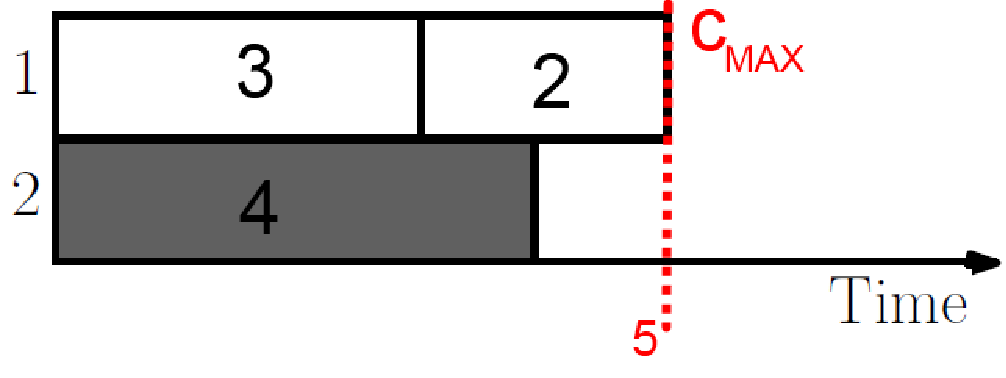
\includegraphics[scale=0.3]{spm6.pdf}
    \caption{Solution donnée par l'algorithme}
    \end{center}
\end{figure}
\end{exemple}

\begin{lemme}
Pour toute instance d'un \textbf{\titre{SPM}} telle que $p_1\geq p_2\geq \ldots \geq p_n > \dfrac{c^*_{MAX}}{3}$, l'algorithme \textbf{LPT}
calcule un schedule optimal.
\end{lemme}

\newpage

\begin{thm} L'algorithme \textbf{LPT} est un algorithme de $\frac 4 3$-approximation pour \textbf{\titre{SPM}}.
\begin{proof}[par contradiction]$ $\\
Supposons que le théorème est faux, c'est-à-dire qu'il existe une instance $p_1\geq p_2\geq \ldots \geq p_n$ qui est un contre exemple. \\
Soit un shedule obtenu par l'application de \textbf{LPT} sur cette instance, on peut supposer que la dernière tâche de la liste, $p_n$, est
également la tâche $l$ qui termine le schedule.
\begin{itemize}
\item[$\hookrightarrow$] Si on ne pouvait supposer cela, alors il existe un autre contre-exemple plus petit (= moins de tâches) qui
respecte cette hypothèse. En effet, soit $l$ la dernière tâche du schedule, il suffit alors d'ignorer toutes les tâches $l+1$, $l+2$,
$\ldots$ (on ne modifie pas la valeur de $c_{MAX}$ vu que c'est $l$ qui cause sa valeur).\\
	 $\rightarrow l$ est maintenant la tâche la plus petite. \\
	 \textit{(ceci est vrai car $n>m$)}
	 \begin{exemple}$ $
\begin{figure}[h!]
    \begin{center}
    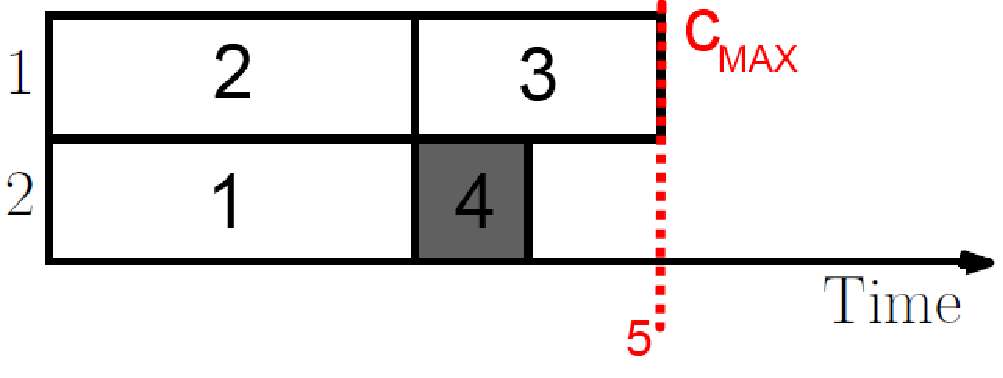
\includegraphics[scale=0.3]{spm8.pdf}
    \caption{Situation considérée}
    \end{center}
\end{figure}
	Ici $l=3$, on ignore donc $4$.
	 \end{exemple}
\end{itemize}
\textbf{Que savons nous de $p_n$ ?}
\begin{enumerate}
\item[a)] si $p_n \leq \frac{C^*_{max}}{3}$

\begin{figure}[h!]
    \begin{center}
    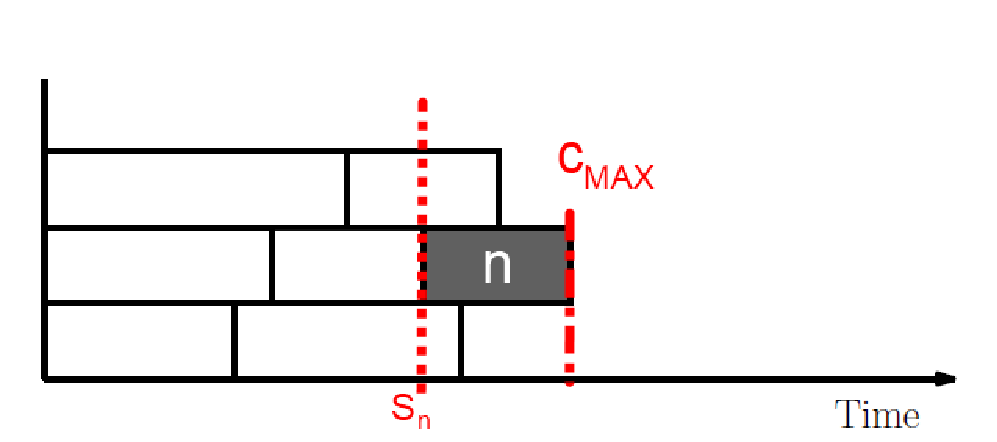
\includegraphics[scale=0.45]{spm7.pdf}
    \caption{Situation considérée}
    \end{center}
\end{figure}
Et donc on a :
\begin{eqnarray}
\nonumber c_{MAX} & = & S_n + p_n \\
\nonumber        &\leq & c^*{MAX} + p_n \\
\nonumber        & < & c^*{MAX} + \frac{c^*{MAX}}{3} = \frac{4}{3}c^*{MAX}
\end{eqnarray}
\item[b)] si $p_n > \frac{c^*_{MAX}}{3}$, par le lemme précédent, \textbf{LPT} donne la solution optimale.
\end{enumerate}
\cqfd
\end{proof}
\end{thm}

\newpage

\subsection{Traveling Saleman Problem (TSP)}

\begin{pblm} \textbf{MIN Traveling Saleman Problem (\titre{TSP})}
\begin{itemize}
\item[*]\textbf{\underline{Instance}} : ensemble de ville = $\{1,2,\ldots,n\}$
ainsi qu'une matrice de distances (ou coûts) $C = C_{ij}$.\\
$\quad\hookrightarrow$ \textbf{\underline{Hypothèses} :} coûts \textbf{symétriques} et \textbf{non négatifs} ($\forall i,j\  C_{ij} =
C_{ji} \geq 0$) et $\forall i,\ C_{ii} = 0$.
\item[*]\textbf{\underline{Solution}} : Un tour de villes, i.e. une permutation
des nombres de 1 à n (on note k(1),k(2), ..., k(n)).
\item[*]\textbf{\underline{Mesure}} : $\left[\sum_{i=1}^{n-1}C_{k(i)k(i+1)}\right] + C_{k(n)k(1)}$
\end{itemize}
\end{pblm}

\begin{rem} De manière équivalente, on peut décrire une instance via un graphe
complet non dirigé et pondéré avec les coûts/distances.
\end{rem}

\begin{exemple}$ $\\
\begin{figure}[h!]
    \begin{center}
    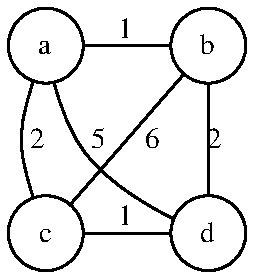
\includegraphics[scale=0.65]{TSPex1.pdf}
    \caption{Exemple d'instance de \textbf{\titre{TSP}} sour forme de graphe pondéré}
    \end{center}
\end{figure}
\begin{itemize}
\item le tour optimal est $a b d c$ et son coût est $6$,
\item $(n-1)!$ possibilités (pas $n!$ car on peut considérer que la première ville est fixée),
\item l'instance n'est pas métrique, c'est-à-dire qu'elle ne respecte pas l'inégalité triangulaire.\\
(En effet, $C_{ab} + C_{bd} \geq C_{ad}$ est faux car $1+2 = 3 < 5$)
\end{itemize}
\end{exemple}

Ce problème nous fait penser à un problème déjà vu lors des années précédentes, le problème de décision consistant à savoir si un graphe
possède un cycle hamiltonien \textit{(cycle passant une et une seule fois par tous les sommets)}. Voyons si on peut effectuer un
rapprochement entre les deux. \\

\begin{pblm} \textbf{Problème Cycle-Hamiltonien?}
\begin{itemize}
\item[*]\textbf{\underline{Instance}} : Graphe $G=(V,E)$ non dirigé.
\item[*]\textbf{\underline{Question}} : $G$ possède-t-il un cycle hamiltonien ?
\end{itemize}
\end{pblm}

\begin{exemple} Existe-t-il un cycle hamiltonien dans un cube ? \\
\begin{figure}[h!]
    \begin{center}
    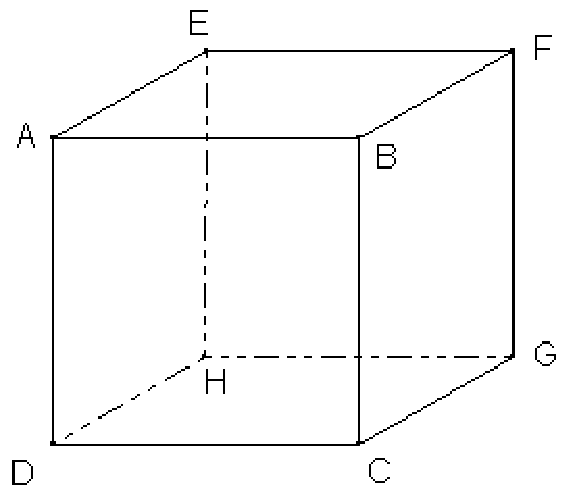
\includegraphics[scale=0.3]{cube.pdf}
    \caption{Cube}
    \end{center}
\end{figure}
$\Longrightarrow$ oui, voir figure~\ref{chcube}.
\begin{figure}[h!]
    \begin{center}
    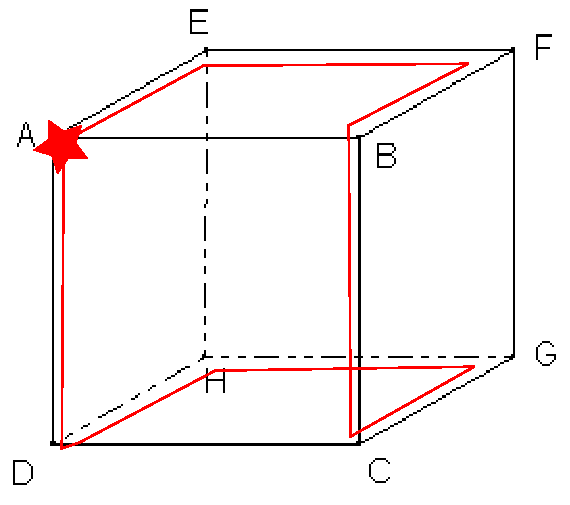
\includegraphics[scale=0.3]{cubehc.pdf}
    \caption{Chemin hamiltonien dans un cube}
    \label{chcube}
    \end{center}
\end{figure}

(il en existe plusieurs)

\end{exemple}

Comment pourrait-on passer du problème du cycle Hamiltonien au \textbf{\titre{TSP}} ? \\
$\hookrightarrow$ A partir de $G=(V,E)$ \textit{(instance du problème Hamiltonien)}, on construit une instance \textbf{\titre{TSP}} comme
ceci :
\begin{itemize}
\item $c_{ij} = 1$ si $(i,j)\in E$
\item $c_{ij} = n+2$ sinon
\end{itemize}
La valeur optimale du \textbf{\titre{TSP}} sur cette instance devrait être égal à $n$, cela signifiant qu'il existe un cycle hamiltonien.
Sinon la solution optimale du \textbf{\titre{TSP}} $\geq (n-1)+(n+2) = 2n+1$ vu qu'il faut au moins sélectionner une arête qui n'existait
pas dans l'instance du cycle. \\

Cette remarque nous dit qu'avec un algorithme de $2$-approximation pour le \textbf{\titre{TSP}}, on pourrait résoudre un problème
\textbf{NP-complet} ! Ce facteur $2$ vient du cout que l'on a placé pour les arêtes inexistantes. On peut donc le faire croître
arbitrairement $\Rightarrow$ il n'existe donc pas d'algorithmes d'approximation pour le \textbf{\titre{TSP}}. Pour s'en convaincre, il
suffit de modifier l'instance précédente en plaçant comme coût pour les arêtes inexistantes un coût égal à $(\alpha-1)n+2$ et ce $\forall
\alpha>1$. On obtient donc :
\begin{eqnarray}
\nonumber OPT & = & n \text{ s'il existe un cycle hamiltonien} \\
\nonumber & = & (n-1) + (\alpha-1)n+2 = \alpha n +1 \text{ sinon}
\end{eqnarray}

Ceci nous amène à une conclusion plutôt décevante, décrite dans le théorème suivant.

\begin{thm}
Pour tout $\alpha > 1$, il n'y a pas d'algorithme d'approximation pour \textbf{\titre{TSP}}, à moins que $\mathcal{P=NP}$.
\end{thm}

\begin{rem}
Ce résultat est dû au fait que les instances considérées ne sont pas métriques. Nous allons donc nous restreindre au \textbf{\titre{TSP}}
métrique.
\end{rem}

\begin{exemple}(\textbf{\titre{TSP}} métrique)
\begin{itemize}
\item $c(i,j) = 1$
\item $c(j,k) = 1$
\item $c(i,k) = 2$
\end{itemize}
$\Rightarrow$ on ne peut mettre plus de $2$ pour $c(i,k)$ sinon on ne respecte pas l'inégalité triangulaire.\\
Dans le cas du \textbf{\titre{TSP}} non métrique, on mettait $(\alpha-1)n+2$ ... !
\end{exemple}

Développons une approche gloutone pour résoudre \textbf{\titre{TSP}}.\\
On note $S$ la permutation finale et $S_i$ la permutation partielle contenant que $i$ villes.\\
Nous allons construire la solution $S$ en ajoutant à chaque itération la ville la plus proche de l'ensemble des villes déja construite.\\
Voici cet algorithme, il est polynomial.

\begin{algorithm}[h!]
\caption{NearestAddition}
\begin{algorithmic}[1]
\STATE $i,j \leftarrow arg\min_{i,j\in S} C_{ij}$
\STATE $tour \leftarrow [i,j]$
\STATE $reste \leftarrow S \setminus \{i,j\}$
\WHILE{$reste \neq \emptyset$}
\STATE $i,j \leftarrow arg\min_{i\not\in reste,j\in reste} C_{ij}$
\STATE insérer $j$ dans $tour$ après $i$
\STATE $reste\leftarrow reste\{j\}$
\ENDWHILE
\end{algorithmic}
\end{algorithm}

\begin{exemple}Les villes de Belgique\\
\begin{figure}[h!]
    \begin{center}
    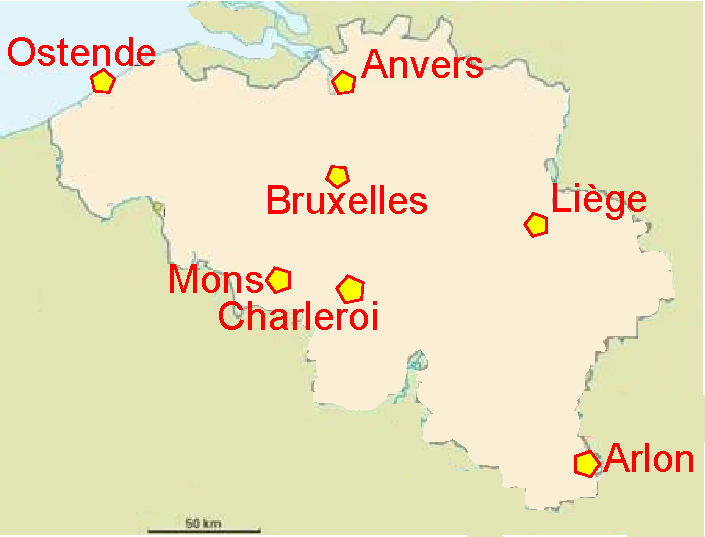
\includegraphics[scale=0.5]{belgique.pdf}$ $\\$ $\\
    \begin{tabular}{r|c|c|c|c|c|c|}
	 & Arlon & Bruxelles & Charleroi & Liège & Mons & Ostende \\
	\hline
	Anvers & 230 & 47 & 105 & 133 & 110 & 119 \\
	& Arlon & 187 & 172 & 127 & 209 & 308 \\
	& & Bruxelles & 60 & 97 & 67 & 113 \\
	& & & Charleroi & 94 & 50 & 167 \\
	& & & & Liège & 127 & 211 \\
	& & & & & Mons & 145
	\end{tabular}
    \caption{Carte et distances de la Belgique}
    \end{center}
\end{figure}
$ $\\
Appliquons l'algorithme \textbf{NearestAddition} : \\
On commence par $S_2 = [Anvers,Bruxelles]$, et on cherche la distance $d_{ij}$ la plus petite telle que $i\in S_k$ et $j \not\in S_k$.\\
On trouve $d_{ij} = 60$ pour Bruxelles-Charleroi. On a donc $S_3 = [Anvers,Bruxelles,Charleroi]$.\\
On itère et on trouve :
\begin{itemize}
\item $S_4 = [Anvers,Bruxelles,Charleroi,Mons]$
\item $S_5 = [Anvers,Bruxelles,Charleroi,Liege,Mons]$
\item $S_6 = [Anvers,Bruxelles,Ostende,Charleroi,Liege,Mons]$
\item $S_7 = S = [Anvers,Bruxelles,Ostende,Charleroi,Liege,Arlon,Mons]$
\end{itemize}
La valeur de la solution est : \textbf{867}. \\
\textit{(La valeur optimale est de \textbf{757}, en prenant $S^* = [Anvers,Bruxelles,Liege,Arlon,Charleroi,Mons,Ostende]$)}
\end{exemple}
\begin{figure}[h!]
    \begin{center}
    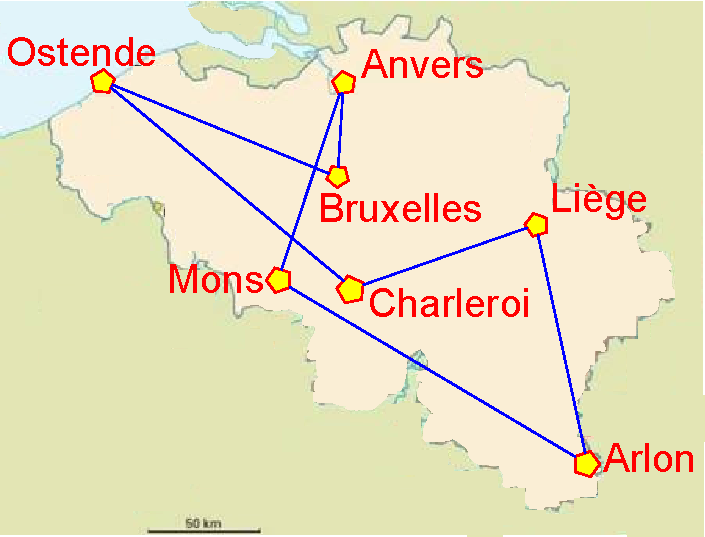
\includegraphics[scale=0.5]{belgiqueNA.pdf}
    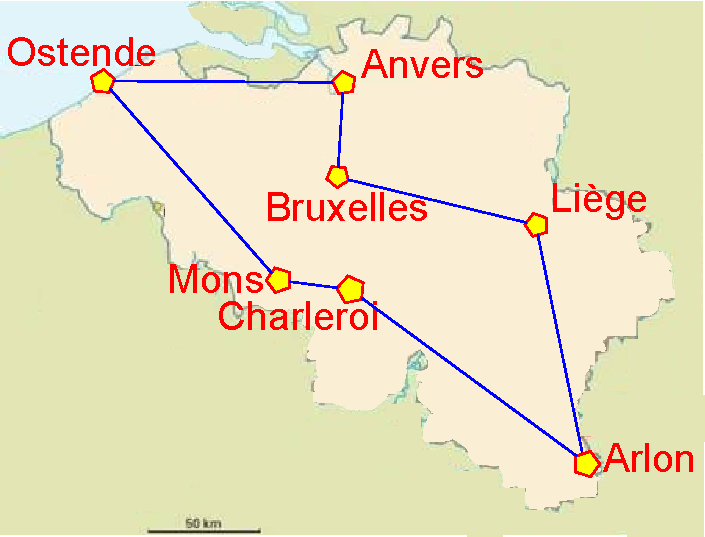
\includegraphics[scale=0.5]{belgiqueOPT.pdf}
    \caption{Solution approchée par \textbf{NearestAddition} et solution optimale}
    \end{center}
\end{figure}

Le coeur de l'analyse de cette algorithme nous amènera à une relation avec la notion d'\textit{arbre couvrant minimum} \textit{(Min
Spanning Tree (\textbf{\titre{MST}}))}. Un arbre couvrant d'un graphe connexe $G=(V,E)$ est un sous-ensemble minimal d'arêtes $F\subseteq
E$ tel que $\forall i,j \in V$, il existe un chemin n'utilisant que des arêtes de $F$ allant de $i$ à $j$. Ce problème appartient à $P$ et
l'algorithme de \textbf{Prim} est un algorithme exact polynomial permettant de le résoudre.

\begin{exemple}$ $
\begin{figure}[h!]
    \begin{center}
    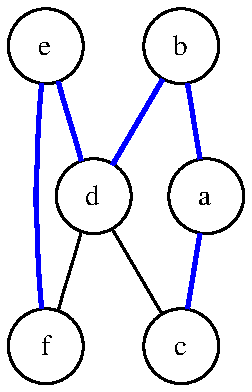
\includegraphics[scale=0.5]{spanningtree.pdf}
    \caption{Graphe et arbre couvrant}
    \end{center}
\end{figure}
\end{exemple}

\begin{pblm}
\textbf{MIN Spanning Tree (\titre{MST})}
\begin{itemize}
\item[*]\textbf{\underline{Instance}} : Graphe $G=(V,E)$ pondéré,
\item[*]\textbf{\underline{Solution}} : Arbre couvrant $F\subseteq E$,
\item[*]\textbf{\underline{Mesure}} : $\sum_{(i,j)\in F} C_{ij}$
\end{itemize}
\end{pblm}

\begin{algorithm}[h!]
\caption{Prim (pour \titre{MST})}
\begin{algorithmic}[1]
\STATE $S\leftarrow\{v\}$ où $v$ est un noeud arbitraire.
\STATE $F \leftarrow \emptyset$
\WHILE{$|S|<|V|$}
\STATE $i,j \leftarrow arg\min_{i\in S,j\not\in S} C_{ij}$
\STATE $F\leftarrow F\cup \{(i,j)\}$
\STATE $S\leftarrow S\cup \{j\}$
\ENDWHILE
\end{algorithmic}
\end{algorithm}

\begin{exemple}
Appliquons l'algorithme de \textbf{Prim} sur l'algorithme de la Belgique.
Il va sélectionner les arêtes :
$$\text{(Ostende,BXL), (Anvers,BXL), (BXL,Charleroi), (Charleroi,Mons), (Charleroi,Liège), (Liège,Arlon)}$$
soit exactement les mêmes que \textbf{NearestAddition}.
\end{exemple}

\begin{lemme}\label{optgeqmst}
Pour toute instance du \textbf{\titre{TSP}} métrique, $OPT \geq \titre{\mathbf{MST}}$.
\begin{proof}
Soit $n\geq 2$, une instance de TSP métrique et son tour optimal :
\begin{figure}[h!]
    \begin{center}
    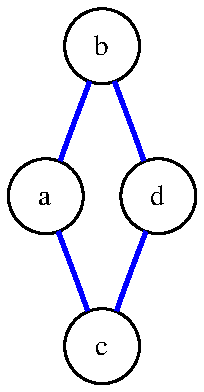
\includegraphics[scale=0.42]{optTSP.pdf}
    \caption{Instance \textbf{\titre{TSP}} métrique et son tour optimal}
    \end{center}
\end{figure}
Supprimer une arête du tour \textbf{OPT} donne un arbre couvrant de poids $w\leq OPT$, or $MST\leq w$ par définition du problème
\textbf{\titre{MST}} et donc $MST\leq OPT$.
\end{proof}
\cqfd
\end{lemme}

\begin{thm}
L'algorithme \textbf{NearestAddition} est un algorithme de $2$-approximation pour le problème \textbf{\titre{TSP}} métrique.
\begin{proof}$ $\\
Soient
\begin{itemize}
\item $S_2$, $S_3$, $\ldots$, $S_n=\{1,\ldots,n\}$ où $S_k$ est le sous ensemble de sommets inclus dans le tour à une itération telle que
$|S_k|=k$,
\item $F = \{ (i_2,j_2), (i_3,j_3), \ldots, (i_n,j_n)\}$ où $(i_l,j_l)$ sont les ``$i$'' et ``$j$'' identifiés dans la boucle de \\
\textbf{NearestAdd} \textit{(ce sont les mêmes que pour \textbf{Prim})}. \\
\end{itemize}

\noindent $T = (S,F)$ est un arbre couvrant de $G=(S,E)$ et on sait que $co\hat{u}t(T) = \sum_{l=2}^n C_{i_lj_l} = MST$.\\
$\hookrightarrow$ Quel est le coût maximimal du tour construit par \textbf{NearestAdd} ?
\begin{itemize}
\item[$\rightarrow$] le premier tour sur $i_2$ et $j_2$ = $2C_{i_2j_2}$ (aller-retour).
\item[$\rightarrow$] Soit une itération où $j$ est inséré entre $i$ et $k$. La différence de coût est donnée par :
$$C_{ij}+C_{jk}-C_{ik}\quad (\star )$$
\begin{center}\textit{(ajout des 2 nouvelles arêtes, suppression de l'ancienne)}\end{center}
Par l'inégalité triangulaire, on sait que $C_{jk}\leq C_{ji} + C_{ik}$ et donc que
$$C_{jk}-C_{ik} \leq C_{ij}\quad (\star\star )$$

Le coût supplémentaire de cette itération est alors : $C_{ij}+C_{jk}-C_{ik}$ qui est borné par $2C_{ij}$ par $(\star\star )$. \\
\end{itemize}

\noindent $\Rightarrow$ En conclusion, $APP$ (coût du tour final donné par \textbf{NearestAdd}) est tel que :
\begin{eqnarray}
\nonumber APP &\leq& 2\ \sum_{l=2}^n C_{i_lj_l} \\
\nonumber     & =  & 2\ MST \\
\nonumber     & \leq & 2\ OPT \text{\textit{(par le lemme \ref{optgeqmst})}}
\end{eqnarray}
\end{proof}
\cqfd
\end{thm}

On peut également imaginer une autre approche avec les \textbf{multigraphes}, c'est-à-dire des graphes autorisant l'existence de plusieurs
arêtes (ici $2$) entre $2$ sommets.

\begin{exemple}$ $\\
\begin{figure}[h!]
    \begin{center}
    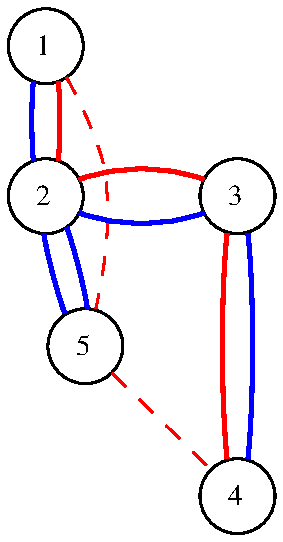
\includegraphics[scale=0.45]{multig.pdf}
    \caption{Exemple de multigraphe}
    \end{center}
\end{figure}

\noindent Ce multigraphe est \textbf{Eulérien}, c'est-à-dire qu'il existe une chemin empruntant chaque arête 1 et une seule fois.\\
Essayons de trouver un tour sur ce graphe (en rouge) :
\begin{itemize}
\item on part de $1$ et on va en $2$, de $2$ à $3$, de $3$ à $4$,
\item on veut retourner en $3$ mais déjà visité, on va donc prendre un \textbf{raccourci} et aller directement en $5$,
\item on veut retourner en $2$ mais déjà visité $\rightarrow$ aller directement en $1$, bouclant ainsi le tour.
\end{itemize}
\end{exemple}

\newpage

Revenons sur la théorie des \textit{cycles Eulériens}, via le problème de \textbf{Konïgsberg}.
\begin{exemple}$ $ \\
\begin{figure}[h!]
    \begin{center}
    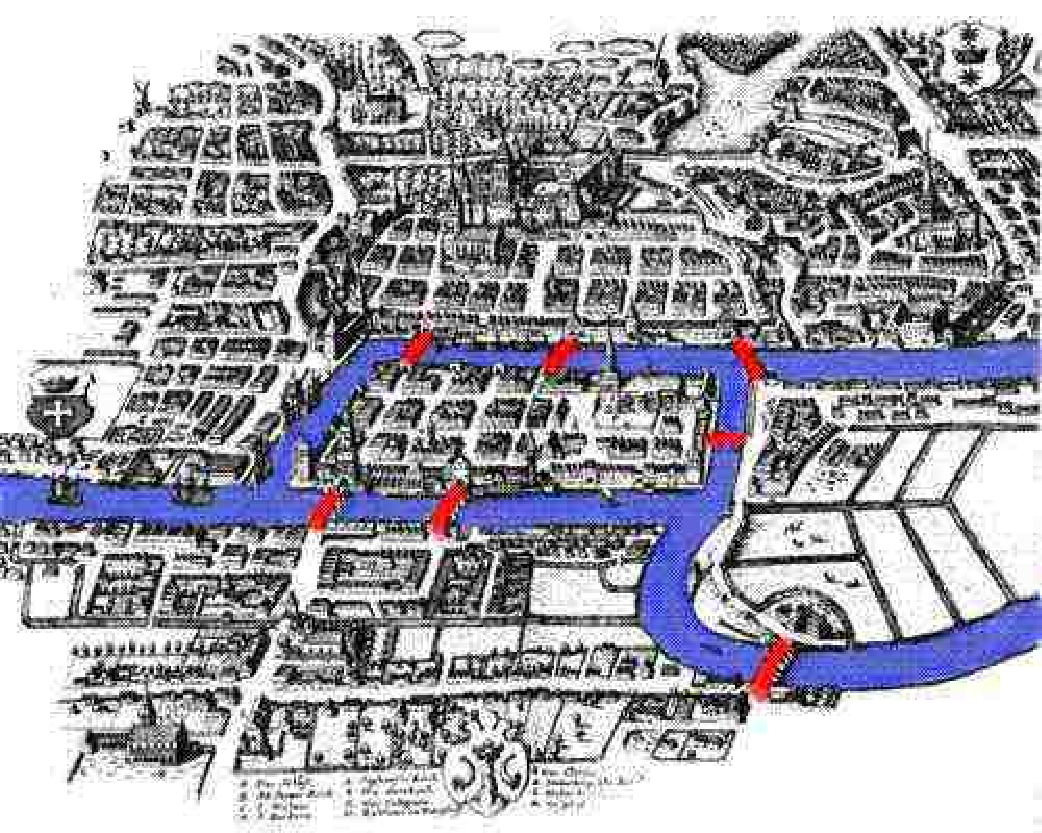
\includegraphics[scale=0.4]{konigsberg.pdf}$\qquad\qquad$
    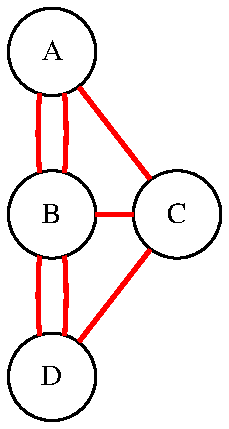
\includegraphics[scale=0.5]{konig.pdf}
    \caption{Plan de la ville de Konïgsberg et le multigraphe associé}
    \end{center}
\end{figure}

Euler a dit en \textbf{1736} qu'une promenade passant une et une seule fois par chacun des ponts est impossible.
Celui-ci n'avait pas utilisé la théorie des graphes pour prouver cela mais cela est facilement visible via un multigraphe où un noeud
correspond à une île/rive et chaque pont est une arête.
\end{exemple}

\begin{de}
Un graphe est \textbf{eulérien} si et seulement si tous les sommets du graphes ont un degré pair et que le graphe est connexe.
\end{de}

\noindent Le problème Eulérien $\in \mathcal{P}$, on peut donc l'utiliser pour approximer \textbf{\titre{TSP}}.\\
Pour trouver un ``bon'' tour pour le \textbf{\titre{TSP}} nous allons :
\begin{enumerate}
\item[a)] calculer un \textbf{\titre{MST}},
\item[b)] remplacer chaque arête par 2 copies $\Rightarrow$ multigraphe eulérien dont le coût est égal à $2\ MST\leq 2\ OPT$
(il est eulérien vu que tous les degrés sont multipliés par 2)
\item[c)] créer un tour qui utilise des "raccourcis" s'il le faut. \\
$\Rightarrow$ à partir d'un cycle eulérien, ne garder que les villes/sommets du parcours quand elles apparaissent pour la première fois
$\Rightarrow$ ``\textbf{Shortcut}''\\
\end{enumerate}
On peut calculer une borne sur la longueur du tour obtenu en c). Les villes ommises n'augmentent pas le coût du multigraphe eulérien. \\
\textit{(via l'inégalité triangulaire, si on prend un raccourci, on diminue (ou conserve) le coût)} \\
$\Rightarrow APP \leq 2\ OPT$, vu que la solution en c) $\leq$ celle en b) qui elle est $\leq 2\ OPT$. \\
$\Longrightarrow$ On a donc un algorithme de $2$-approximation, on l'appellera \textbf{DoubleTree}.

\begin{thm}
L'algorithme \textbf{DoubleTree} est un algorithme de $2$-approximation pour \textbf{\titre{TSP}}.
\begin{proof} (cf analyse ci-dessus)
\end{proof}
\cqfd
\end{thm}

\begin{algorithm}[h!]
\caption{Double Tree}
\begin{algorithmic}[1]
\STATE $MST\leftarrow PRIM(G)$
\STATE $DT \leftarrow double\_edges(MST)$
\STATE $walk \leftarrow eulerian\_walk(DT)$
\STATE $tour \leftarrow shortcut(walk)$
\RETURN $cost(tour)$
\end{algorithmic}
\end{algorithm}

\begin{exemple} Appliquons \textbf{Double Tree} sur l'exemple de la Belgique. \\
On a déjà appliqué \textbf{Prim} précédemment (même résultat que \textbf{NearestAddition}), on a donc : \\
$	F = \{(Anvers,Bruxelles),\ (Charleroi, Anvers),\ (Mons, Charleroi),\ \\\indent\quad  (Liege, Charleroi),\ (Ostende, Bruxelles),\ (Arlon,
Liege)\} $ \\
On obtient donc l'arbre couvrant avec les arêtes données par $F$. $\Rightarrow$ 3 raccourcis apparaissent :
$$Arlon-Mons\qquad Mons-Ostende\qquad Ostende-Anvers$$
On obtient le tour $Anvers-Bruxelles-Charleroi-Liege-Arlon-Mons-Ostende = 801km$.
\begin{figure}[h!]
    \begin{center}
    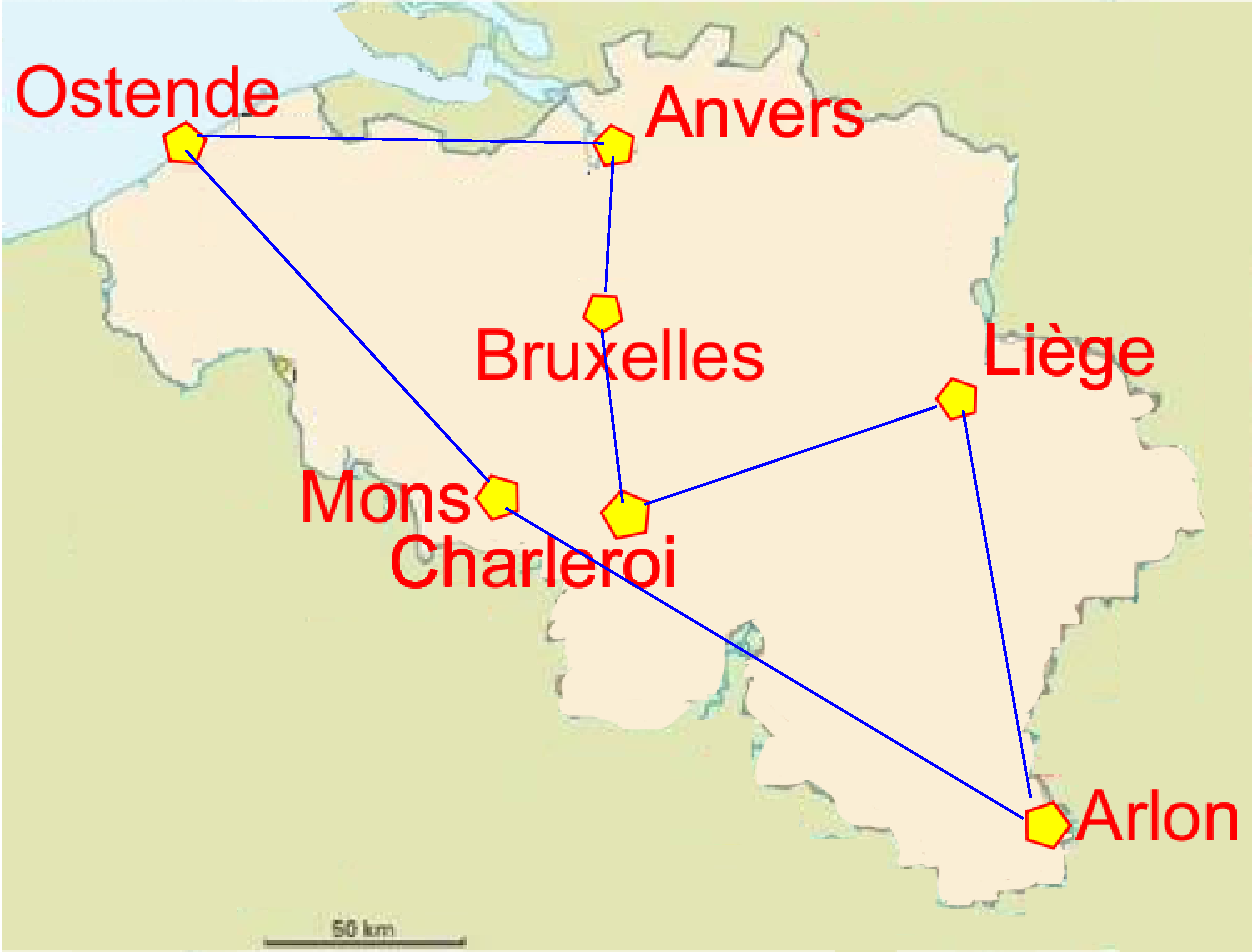
\includegraphics[scale=0.28]{belgiqueDT.pdf}
    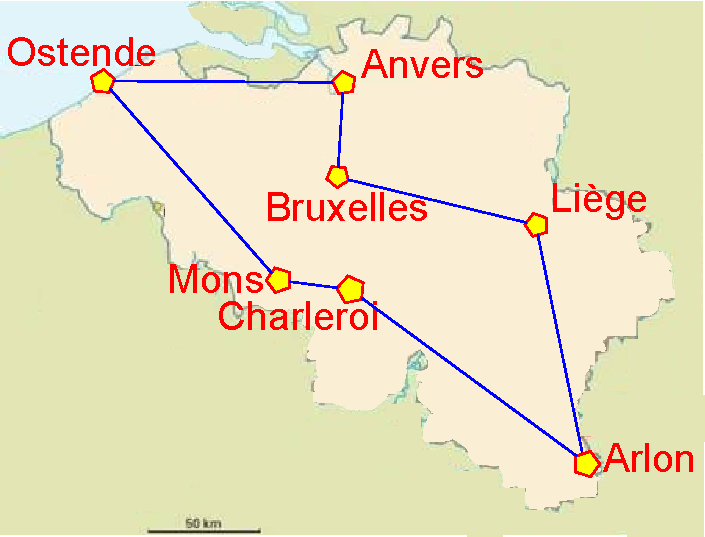
\includegraphics[scale=0.5]{belgiqueOPT.pdf}
    \caption{Solution approchée par \textbf{DoubleTree} et solution optimale}
    \end{center}
\end{figure}
\end{exemple}

L'idée clé utilisée pour prouver que l'algorithme est un algo de $2$-approximation est que le cycle dans un graphe eulérien a un coût
inférieur à $2\ OPT$. Donc, si on trouve un meilleur graphe eulérien, c'est-à-dire un graphe eulérien tel que le coût du cycle est $\leq
\alpha OPT$, alors l'algorithme est d'$\alpha$-approximation. Il existe en effet un meilleur algorithme, donné par \textit{Christophides},
qui est le meilleur algorithme connu à ce jour et qui a un facteur $\frac 3 2$. \\
Parlons d'abord des degrés des sommets d'un graphe et énonçons quelques propriétés :
\begin{enumerate}
\item La somme des degrés d'un graphe, $\Delta(G) = 2m$ où $m$ est le nombre d'arêtes car chaque arête est comptée 2 fois (ses 2
extrémités).
\item La somme des degrés est donc toujours \textbf{paire}.
\item La somme des degrés des sommets ayant un degré pair est toujours paire car c'est une somme de nombres pairs.
\item La somme des degrés des sommets ayant un degré impair est toujours paire. \textit{(par 2. et 3., sinon la somme totale serait
impaire)}
\item Le nombre de sommets de degrés impairs est pair. \textit{(par 4.)}
\end{enumerate}
Dans la suite, nous noterons $O$ l'ensemble des sommets de degré impair d'un graphe.

\begin{exemple}Vérifions ces propriétés sur le graphe G (figure \ref{grapheg}).\\
Le graphe possède $7$ noeuds et $6$ arêtes et les degrés sont :
\begin{center}
\begin{tabular}{c|c}
Sommet $i$ & Degré de $i$ $d(i)$ \\
\hline
$1$ & $2$ \\
$2$ & $1$ \\
$3$ & $3$ \\
$4$ & $1$ \\
$5$ & $2$ \\
$6$ & $2$ \\
$7$ & $1$ \\
\end{tabular}
\end{center}
\begin{itemize}
\item $\sum{d(i)} = 12 = 2\ast6 =$ $2$ fois le nombre d'arêtes et c'est pair.
\item $4$ sommets de degrés impairs et la somme de leur degré $\rightarrow 1+3+1+1 = 6$, c'est pair.
\item $O = {2,3,4,7}$ et $|O| = 2*k$ (par 5)) pour un entier $k$ non négatif (ici $k=2$).
\end{itemize}
\begin{figure}[h!]
    \begin{center}
    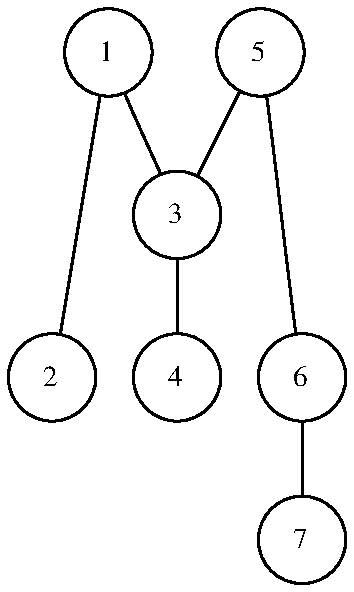
\includegraphics[scale=0.5]{degre.pdf}
    \caption{Graphe G}
    \label{grapheg}
    \end{center}
\end{figure}
\end{exemple}

\newpage

Supposons qu'on groupe les sommets de degrés impairs par paires (ce qui est possible car $|0| = 2k$) : $(i_1,i_2)$, $(i_3,i_4)$ ...
$(i_{2k-1},i_{2k})$. On obtient ainsi un \textbf{perfect matching}, c'est-à-dire un ensemble d'arêtes non incidentes entre elles qui
couvrent tous les sommets (ici, tous les sommets de $O$).

\begin{exemple} Dans l'exemple précédent, associons $(2,3)$ et $(4,7)$ et on obtient un graphe avec des sommets comportants uniquement des
sommets de degrés pairs.
\end{exemple}

\noindent Il existe plusieurs \textbf{perfect matching} \textit{(et plus k est grand plus il y en a)} \\
$\Longrightarrow$ le problème \textbf{MIN Perfect Matching} consiste à trouver le perfect matching de coût minimum. \\
$\rightsquigarrow$ Il existe un algorithme polynomial pour résoudre ce problème, l'algorithme d'\textbf{Edmonds} en $O(n^4)$.\\
\textit{(voire $O(n^3)$ avec des SDD particulières)}

\begin{algorithm}[h!]
\caption{Christophides (informel)}
\begin{algorithmic}[1]
\STATE $MST\leftarrow PRIM(G)$
\STATE $O \leftarrow$ ensemble des sommets impairs de $MST$
\STATE $PM\leftarrow compute\_perfect\_matching(O)$
\STATE $EG\leftarrow MST\cup PM$
\STATE $tour \leftarrow shortcut(EG)$
\RETURN $cost(tour)$
\end{algorithmic}
\end{algorithm}

\begin{rem} \textbf{EG} est eulérien car il est connexe vu que \textbf{MST}  l'était déjà et tous les degrés sont pairs puisque
l'algorithme a ajouté exactement une arête à chaque sommet de degré impair, via le \textbf{perfect matching}.
\end{rem}

\begin{exemple} Appliquons \textbf{Christophides} sur l'exemple de la Belgique. \\
\begin{figure}[h!]
    \begin{center}
    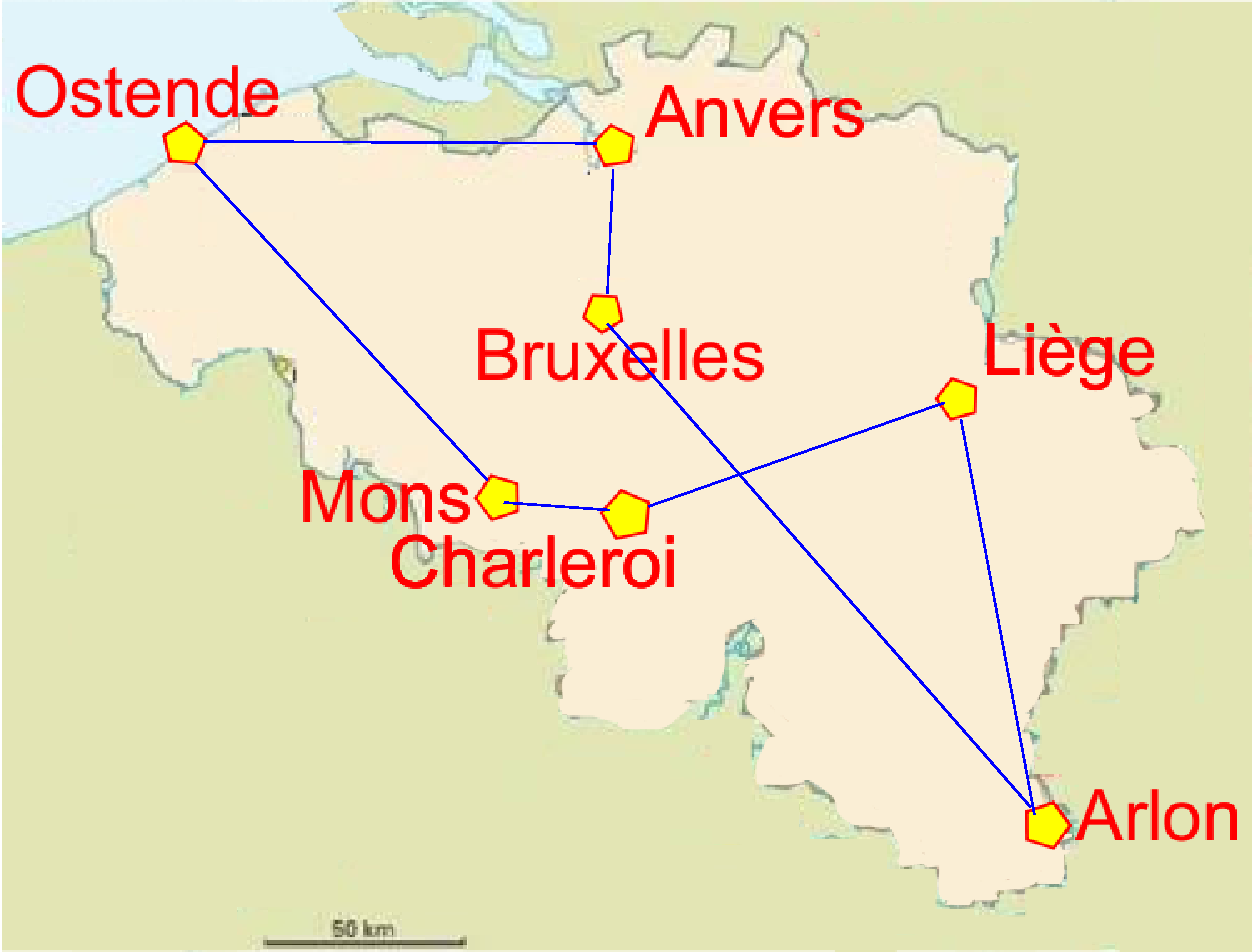
\includegraphics[scale=0.28]{belgiqueCHRIS.pdf}
    \includegraphics[scale=0.5]{belgiqueOPT.pdf}
    \caption{Solution approchée par \textbf{Christophides} et solution optimale}
    \end{center}
\end{figure}

\noindent Seul Liège a un degré pair. \\
Le meilleur \textbf{PM} est : $Anvers-Ostende$, $Charleroi-Mons$, $Bruxelles-Arlon$, avec un poids de $356$ km. \\
Chistophides donne donc le tour : \\ $Anvers-Bruxelles-Arlon-Liege-Charleroi-Mons-Ostende \rightarrow 769$km. \\
\textit{(Rappel : $OPT = 757$ km)}
\end{exemple}

\begin{thm}L'algorithme de Christophides est un algorithme de $\frac 3 2$-approximation pour le problème \textbf{\titre{TSP}-métrique}.
\begin{proof}$ $\\
Il reste à prouver que le graphe eulérien EG a un coût total $\leq \frac 3 2 OPT$. \\
On sait que $cout(EG) = cout(MST) + cout(PM)$ et que $cout(MST)\leq OPT$, on doit donc prouver : $$cout(PM)\leq \frac{OPT}{2}$$.
\begin{enumerate}
\item[a)] Observons d'abord qu'il existe un tour sur les sommets de $O$ qui a un coût $\leq OPT$. Soit un tour optimal sur toutes les
villes, il suffit de prendre des shortcuts sur ce tour optimal pour obtenir un tel tour. Et via les arguments déjà cités (inégalité
triangulaire), le tour ainsi créé est $\leq OPT$.
\item[b)]$ $
\begin{figure}[h!]
    \begin{center}
    \includegraphics[scale=0.5]{pmO.pdf}
    \caption{Exemple de tour sur $6$ villes $\in O$}
    \end{center}
\end{figure}
Sur ce tour, il y a 2 \textbf{Perfect Matching} (pour rappel, il s'agit d'un ensemble d'arêtes non incidentes entre elles
couvrant chaque noeud) (on numérote les arêtes) soit en prenant les arêtes numérotées impaires soit en prenant les arêtes numérotées
paires.\\
Vu que la somme des couts de ces 2 perfect matching $\leq OPT$, au moins un des 2 (le minimum perfect matching est peut-être encore plus
petit) est tel que $PM \leq \frac{OPT}{2}$.
\end{enumerate}
\cqfd
\end{proof}
\end{thm}

Ce facteur d'approximation est serré, nous allons le montrer sur l'exemple suivant.

\begin{exemple}$ $\\
\begin{figure}[h!]
    \begin{center}
    \includegraphics[scale=0.5]{factserre.pdf}
    \caption{Exemple serré pour le facteur d'approximation}
    \end{center}
\end{figure}

Si le tour ne prend que les arêtes vertes, on obtient la solution optimale dont le coût est :
$$(n-1) + 4(1+\epsilon) + (n-2) = 2n - 1 + 4\epsilon$$

Seulement, si l'arbre couvrant donné par l'algorithme est toutes les arêtes rouges (+ les 2 arêtes vertes extérieures), il n'y a que $2$
sommets de degrés impairs : $a_1$ et $a_{n+1}$. Le \textbf{perfect matching} va donc devoir les relier, on obtient alors une solution dont
la valeur est : $$ 2(1+\epsilon) + 2(n-1) +      n       = 3n+2\epsilon $$

Le ratio est donc : $$\dfrac{3n+2\epsilon}{2n+4\epsilon-1} \to_{n\to\infty} \dfrac{3}{2}$$
\end{exemple}

$\Longrightarrow$ \textbf{Il n'y a pas de meilleur d'algorithme d'approximation à ce jour pour le \titre{TSP} métrique.}

\begin{thm}[Résultat d'inapproximabilité pour \titre{TSP}]$ $\\
A moins que $\mathcal{P=NP}$, pour toute constante $\alpha \leq \frac{220}{219}\simeq 1,0045$, il n'existe pas d'algorithme d'approximation
pour le \textbf{\titre{TSP}} métrique.
\end{thm}

\vspace{47em}
\begin{flushright}
$\hookrightarrow$ \begin{large}Voir exercices dans l'annexe~\ref{exoChap3}.\end{large}
\end{flushright}

\newpage

\section{Programmation dynamique et arrondissement (rounding) de données}

La programmation dynamique est une technique classique en algorithmique où une solution optimale est construite à partir de solutions
optimales de sous-problèmes, en général stockées dans une table ou un tableau multidimensionnel. Nous allons utiliser cette technique pour
des problèmes "faiblement" NP-difficiles en ce sens où il existe un algorithme pseudo-polynomial, c'est-à-dire presque polynomial.

\subsection{Le problème du sac à dos (knapsack problem)}

\begin{pblm}
\textbf{MAX sac à dos \titre{\textbf{KP}}}
\begin{itemize}
\item[*]\textbf{\underline{Instance}} :
\begin{itemize}
\item ensemble d'objets $I=\{1,2,\ldots,n\}$, chaque objet a une valeur $v_i$ et
une taille $s_i$,
\item le sac à dos a une capacité $B$;
\end{itemize}
\item[$\hookrightarrow$]\underline{Hypothèses} :
\begin{itemize}
\item toutes les données sont des entiers ($v_i$, $s_i$ et $B$),
\item $\forall i,\ s_i\leq B$
\end{itemize}
\item[*]\textbf{\underline{Solution}} : $S\subseteq I$ tel que $\sum_{i\in S}{(s_i)} \leq B$
\item[*]\textbf{\underline{Mesure}} : le profit, c'est-à-dire $\sum_{i\in S}{(v_i)}.$\\
\end{itemize}
\end{pblm}

\noindent \underline{Quelques applications} :
\begin{itemize}
\item utilisé pour minimiser les chutes dans les problèmes de découpe,
\item sélection de porte-feuilles et d'investissements financiers,
\item génération de clés dans le système cryptographique de \textbf{Merkle-Hellman}.
\end{itemize}

\begin{exemple}$ $\\
$I=\{1,2,3,4\}$ \\
$v_1 = 4$, $s_1=2$\\
$v_2 = 5$, $s_2=3$\\
$v_3 = 3$, $s_3=2$\\
$v_4 = 2$, $s_4=1$\\

\noindent $OPT$ pour $B=8$ ? $\rightarrow$ tout prendre $\longrightarrow$ $size = 8$ et $profit = 14$\\
$OPT$ pour $B=6$ ? $\rightarrow$ $\{1,2,4\}$ $\longrightarrow$ $size = 6$ et $profit = 11$\\
$OPT$ pour $B=5$ ? $\rightarrow$ $\{1,2\}$ ou $\{1,3,4\}$ $\longrightarrow$ $size = 5$ et $profit = 9$\\
$OPT$ pour $B=4$ ? $\rightarrow$ $\{1,3\}$ ou $\{2,4\}$ $\longrightarrow$ $size = 4$ et $profit = 7$
\end{exemple}

$ $\\

Pourquoi ne pas essayer un algorithme glouton sur ce problème ? L'idée est de trier les objets selon un ordre choisi puis les ajouter dans
cet ordre dans le sac. Nous allons envisager plusieurs ordres et montrer qu'à chaque ordre il existe une instance où on peut faire aussi
mauvais que possible. \\

\begin{algorithm}[h!]
\caption{GloutonKPGeneral}
\begin{algorithmic}[1]
\STATE Trier les objets selon une certaine règle.
\STATE Placer les objets dans le sac dans cet ordre jusqu'à ce que le sac soit trop plein.
\end{algorithmic}
\end{algorithm}

\textbf{\underline{Les règles possibles}} :
\begin{itemize}
\item \textbf{taille croissante} : on prend un objet de taille $1$ et de valeur $1$ et un objet de taille $B$ et de valeur $M>1$. La valeur
optimale est $M$ et la valeur approchée est $1$. Le ratio est donc $1/M$ et on peut faire grandir $M$ tant que l'on veut.
\item \textbf{valeur décroissante} : on prend un objet de taille $B$ et de valeur $M$ et $B$ objets de taille $1$ et de valeur $M-\epsilon$
($\epsilon$ petit). La valeur optimale est donc $B(M-\epsilon) \sim BM$ (avec $\epsilon\to 0$) et la valeur approchée est $M$. Le ratio est
donc $1/B$ avec $B$ que l'on peut faire grandir tant que l'on veut.
\item \textbf{ratio valeur/taille décroissant} : on prend un objet de taille $1$ et de valeur $1+\epsilon$ et un objet de taille $B$ et de
valeur $B$. La valeur optimale est donc $B$ et la valeur approchée est $1+\epsilon\sim 1$. Le ratio est donc $1/B$ avec $B$ que l'on peut
faire grandir tant que l'on veut.
\end{itemize}

\textbf{$\Rightarrow$ les algorithmes gloutons ne sont pas très bons.} \\

\noindent Posons nous les bonnes questions : dans le cas d'une recherche exhaustive,
\begin{itemize}
\item combien y a-t-il de possibilités ? $\rightarrow 2^n$
\item comment représenter graphiquement cela ? $\rightarrow$ arbre binaire complet où chaque niveau $i$ représente la question "prend-on
l'objet $i$ dans le sac ?".
\end{itemize}

\begin{figure}[h!]
    \begin{center}
    \includegraphics[scale=0.5]{arbredec1.pdf}
    \caption{Arbre de décision type}
    \end{center}
\end{figure}

\begin{exemple}(exemple précédent) La figure \ref{bigtree} contient l'arbre de décision relatif à l'exemple précédent. Chaque noeud contient
un couple $(x,y)$, où $x=$ taille de la solution partielle et $y=$ profit de cette solution partielle. \\

\begin{rems}(sur l'exemple)
\begin{itemize}
\item On peut ne pas énumérer tout l'arbre car à certains niveaux, on a des noeuds qui ont la même taille mais pas le même profit, ce qui
signifie que pour les mêmes éléments avec la même taille on a un meilleur profit, il est donc inutile de générer le reste du sous-arbre
concerné.
\item On peut également avoir une situation identique si on a le même profit et que la taille est plus petite.
\item On peut également supprimer 2 branches donnant la même taille et le même profit, vu que les 2 solutions intermédiaires sont identiques,
on choisit celle que l'on veut.
\end{itemize}
\end{rems}

\begin{figure}[h!]
    \begin{center}
    \includegraphics[scale=0.4]{arbredec2.pdf}
    \caption{Arbre de décision relatif à l'exemple}
    \label{bigtree}
    \end{center}
\end{figure}
\end{exemple}
$ $\\

\noindent \underline{Formalisons nos observations} : soient $P$ et $Q$, $2$ sous-problèmes au ``même niveau''  \\ (i.e. qui ont considérés
les mêmes objets) de $1$ à $j$ :
\begin{itemize}
\item[si] $taille(P) = taille(Q)$
	\begin{itemize}
	\item[si] $profit(P) \geq profit(Q)$ alors calculer $P$
	\item[sinon] calculer $Q$
	\end{itemize}
\item[sinon si] $profit(P) = profit(Q)$
	\begin{itemize}
	\item[si] $taille(P) > taille (Q)$ alors calculer $Q$
	\item[sinon] calculer $P$ \\
	\end{itemize}
\end{itemize}

\noindent Pour \textbf{\titre{KP}} :
\begin{itemize}
\item la notion de sous-problème est simple et naturelle,
\item il y a beaucoup de redondance dans la recherche exhaustive, d'où l'interêt d'avoir des données entières.
\end{itemize}

\newpage

\subsubsection{Programmation dynamique pour \titre{KP} (1ère version)}
\begin{itemize}
\item[$\rightarrow$] on suppose qu'on a considéré les objets de $1$ à $i$,
\item[$\rightarrow$] on veut se souvenir des profits qui sont possibles,
\item[$\rightarrow$] pour chaque profit possible on veut minimiser la taille associée.
\end{itemize}

Nous allons utiliser les notations suivantes,
\begin{itemize}
\item $S(i,p)$ est le sous-ensemble de $I$ tel que le \textbf{profit} est égal à $p$ et la \textbf{taille} est \textbf{minimisée},
\item $A(i,p)$ représente la taille de $S(i,p)$, vaut $\infty$ si il n'existe pas d'ensemble $S(i,p)$.
\end{itemize}

\begin{exemple} \textit{(exemple précédent)}
\begin{eqnarray}
\nonumber A(1,p) & = & s_1 \text{ si }p=v_1 \\
\nonumber 	     & = & 0 \text{ sinon si } p = 0 \\
\nonumber 		 & = & \infty \text{ sinon}
\end{eqnarray}

\newpage

Le tableau $A$ est donc de la forme :
\begin{center}\begin{tabular}{c|cccccc}
$Objet\backslash P$ & $0$ & $1$ & $2$ & $3$ & $4$ & $\ldots$ \\
\hline
$1$ & $0$ & $\infty$ & $\infty$ & $\infty$ & $2$ & $\ldots$ \\
$2$ & $\ldots$ & $\ldots$ & $\ldots$ & $\ldots$ & $\ldots$ & $\ldots$ \\
$3$ & $\ldots$ & $\ldots$ & $\ldots$ & $\ldots$ & $\ldots$ & $\ldots$ \\
$\vdots$ & $\ldots$ & $\ldots$ & $\ldots$ & $\ldots$ & $\ldots$ & $\ldots$ \\
\end{tabular}\end{center}$ $\\
Il y a $V$ colonnes, où $V = \sum_{k=1}^n v_k$ et $n$ lignes, c'est donc une matrice $n\times V$.
\end{exemple}

Nous voulons trouver une formule inductive pour calculer le tableau $A$, c'est-à-dire une formule pour calculer la $(i+1)^{\text{ème}}$ ligne
à partir de la ligne $i$.
\begin{eqnarray}
\nonumber A(i,p) & = & \text{taille minimum pour un profit p en utilisant les $i$ premiers objets}\\
\nonumber A(i+1,p) & = & A(i,p) \text{ si on a pas pris } i+1 \\
\nonumber 		& = & A(i,p-v_{i+1}) + s_{i+1} \text{ si on prend } i+1\\
\nonumber 		& = & \text{en fait le minimum de ces 2 valeurs vu qu'on prend la taille minimum}
\end{eqnarray}

\begin{exemple}
Remplir la table $A(i,p)$ pour l'exemple. \textit{(case blanche = $\infty$)} \\

\begin{tabular}{c|ccccccccccccccc}
$A$ & $0$ & $1$ & $2$ & $3$ & $4$ & $5$ & $6$ & $7$ & $8$ & $9$ & $10$ & $11$ & $12$ & $13$ & $14$ \\
\hline
$1$ & $0$ &   &   &   & $2$ &   &   &   &   &   &    &    &    &    &    \\
$2$ & $0$ &   &   &   & $2$ & $3$ &   &   &   & $5$ &    &    &    &    &    \\
$3$ & $0$ &   &   & $2$ & $2$ & $3$ &   & $4$ & $5$ & $5$ &    &    &  $7$ &    &    \\
$4$ & $0$ &   & $1$ & $2$ & $2$ & $3$ & $3$ & $4$ & $5$ & $5$ &  $6$ &  $6$ &  $7$ &    &  $8$ \\
\end{tabular}
$ $\\

\noindent On peut calculer l'optimum facilement, par exemple pour $B = 6$, le $6$ plus à droite donne $11$.
\end{exemple}

L'algorithme utilisant cette table est donc en $O(n\times V)$, ce qui semble polynomial mais le problème est que $V$ n'est pas une
constante vu qu'elle dépend des valeurs que prennent les entrées. \\
De \textbf{manière intuitive}, si $V$ est beaucoup plus grand que $n$, le nombre de colonnes dans le tableau ne pourra pas être bornée par
un polynôme en $n$. \\
De \textbf{manière plus formelle}, soit ``$size$'' la taille utilisée pour représenter $V$, quelle est la complexité de notre programme
dynamique en fonction de $n$ et ``$size$'' ? Sur nos machines \textit{(binaires)} : $size = \log_2{(V)}$ et donc $V = 2^{size}$,
$\Rightarrow O(n \times 2^{size})$. \\

\begin{de}
Un algorithme \textbf{polynomial} quand les entrées sont représentées sous forme unaire est un algorithme \textbf{pseudopolynomial}.
\end{de}

\begin{rem}
En unaire : $(7)_{10} = (1111111)_1$, et dans ce cas $size = O(V)$ et donc $O(n\times size)$ mais évidemment size peut être énorme.
\end{rem}

\subsubsection{Variation du programme dynamique}

Nous allons utiliser un tableau de listes de paires : \\
$A(j)$ pour $j = 1,...,n$ contient une liste de paires $(t,w)$ où une paire signifie qu'il existe un sous ensemble $S\subseteq I$ utilisant
les $j$ premiers objets avec une \textbf{taille} $t$ et un \textbf{profit} $w$. \\
En d'autres mots si $(t,w)$ est dans la liste $A(j)$, alors il existe $S\subseteq \{1,2,...,j\}$ tel que $\sum_{j\in S} s_i = t \leq B$ et
$\sum_{i\in S} v_i = w$.

\begin{de}
On dit qu'une paire $(t,w)$ \textbf{domine} une paire $(t',w')$ si $t\leq t'$ et
$w \geq w'$. (relation transitive)
\end{de}

Nous allons nous assurer que dans une liste, aucune paire n'en domine une autre. On peut donc supposer que $A(j)$ est de la forme $(t_1,w_1),
\ (t_2,w_2),\ \ldots ,\ (t_k,w_k)$ et est telle que :
\begin{eqnarray}
\nonumber t_1 & < & t_2 < \ldots < t_k \\
\nonumber w_1 & < & w_2 < \ldots < w_k
\end{eqnarray}
$ $\\
$ $\\
$ $\\

\noindent Comme pour tout $i$, $v_i$ et $s_i$ sont des entiers :
\begin{enumerate}
\item[a)] dans chaque liste, il y a au plus $B+1$ paires ($+1$ car il y a la taille $0$)
\item[b)] dans chaque liste, il y a au plus $V+1$ paires ($+1$ car il y a le profit $0$)
\item[c)] pour tout sous-ensemble $S\subseteq \{1,...,j\}$ réalisable (i.e $\sum_{i\in S}(s_i) \leq B$), la liste $A(j)$ contient une paire
$(t,w)$ qui donne la paire ($\sum_{i\in S}(s_i)$,$\sum_{i\in S}(v_i)$).
\end{enumerate}

\begin{algorithm}[h!]
\caption{DynProg\_KP}
\begin{algorithmic}[1]
\STATE $A(1)\leftarrow \{(0,0),(s_1,v_1)\}$
\FOR{$j$ allant de $2$ à $n$}
\STATE $A(j)\leftarrow A(j-1)$
\FOR{chaque paire $(t,w) \in A(j-1)$}
\IF{$t+s_j \leq B$}
\STATE Ajouter ($t+s_j$,$w+v_j$) à $A(j)$
\ENDIF
\ENDFOR
\STATE Retirer les paires dominées de $A(j)$
\ENDFOR
\STATE Retourner $\max_{(t,w)\in A(n)}(w)$
\end{algorithmic}
\end{algorithm}

$\Longrightarrow O(n\times min(B,V))$

\begin{exemple}
\noindent $A(1) \leftarrow \{(0,0),(2,4)\}$ \\
Itération $j = 2$ \\
\indent $A(2) \leftarrow \{(0,0),(2,4)\}$
\indent \begin{itemize}
\item $(0,0)$ : $0+3 \leq_? 5 \rightarrow$ oui donc ajouter $(3,5)$
\item $(2,4)$ : $2+3 \leq_? 5 \rightarrow$ oui donc ajouter $(5,9)$
\end{itemize}
$\ldots$
\end{exemple}

\begin{thm}
\textbf{DynProg\_KP} calcule la valeur exacte pour \textbf{\titre{KP}}.
\end{thm}

\begin{de}
Un \textbf{schéma d'approximation en temps polynomial} (\textbf{PTAS}) est une famille d'algorithmes $\{A_\epsilon\}$ telle qu'il existe un
algorithme pour chaque valeur $\epsilon > 0$ de sorte que $A_\epsilon$ est un algorithme de \\ \indent $\qquad\qquad\qquad \left\{
\begin{array}{c}
(1-\epsilon) \text{ (pour un MAX)}\\
(1+\epsilon) \text{ (pour un MIN)}
\end{array}\right.$-approximation.
\end{de}

\begin{de}
Si pour un \textbf{PTAS} chaque algorithme $A_\epsilon$ a un temps d'exécution borné par un polynome en $\frac{1}{\epsilon}$, alors on parle
de schéma d'approximation complet (\textbf{FPAS}).
\end{de}

\begin{algorithm}[h!]
\caption{FPAS\_KP}
\begin{algorithmic}[1]
\REQUIRE $\epsilon > 0$
\STATE $M \leftarrow \max_{i\in I}(v_i)$
\STATE $\mu \leftarrow \frac{(\epsilon M)}{n}$
\FOR{tous les $i \in I$}
\STATE $v_i' \leftarrow \cdil{(\frac{v_i}{\mu})}$
\ENDFOR
\STATE Exécuter \textbf{DynProg\_KP} sur instance modifiée
\end{algorithmic}
\end{algorithm}

On peut réellement avec cet algorithme donner la précision désirée. Evidemment, plus la précision est grande plus l'algorithme sera lent.
Pour une idée sur la précision, si on prend par exemple $\mu = 100$, on ne fait plus la différence entre la valeur $2000$ et la valeur
$2099$.\\
$ $\\$ $\\$ $\\

$\hookrightarrow$ Comment pouvons-nous être sûrs que la garantie est bien $\epsilon$ ?\\
\underline{Idées} :
\begin{itemize}
\item ``mesurer'' les profits en multiples entiers de $\mu$,
\item exécuter sur instance $(s_i,v_i')$ $\rightarrow$ le nombre de colonnes diminue,
\item retourner la valeur de l'instance modifiée comme la valeur approchée de l'instance originale.
\item $M = \max_{i\in I}(v_i) \Rightarrow M \leq OPT$ \textbf{(1)} \\
\end{itemize}

Pourquoi choisir $\mu = \frac{\epsilon M}{n}$ ?
\begin{itemize}
\item[$\rightarrow$] supposons qu'on accepte une erreur d'au plus $\mu$ pour un profit,
\item[$\rightarrow$] au total on a un profit maximum qui a été changé d'au plus $n\mu$,
\item[$\rightarrow$] on veut que cette erreur ($n\mu$) soit au plus un paramètre $\epsilon$ multiplié par une borne inférieur sur $OPT$ ($M$
par exemple) $\longrightarrow$ Choisissons $n\mu = M\epsilon$.
\end{itemize}

\begin{thm}
L'algorithme \textbf{FPAS\_KP} est un \textbf{FPAS} pour \textbf{\titre{KP}}.
\begin{proof}$ $
\begin{enumerate}
\item[a)] Le temps d'exécution est borné par un polynôme en $\dfrac{1}{\epsilon}$. \\
On observe :
\begin{eqnarray}
\nonumber V' & = & \sum_{i=1}^n(v'_i) \\
\nonumber    & = & \sum_{i=1}^n\cdil{\dfrac{v_i}{\mu}} \\
\nonumber    & = & \sum_{i=1}^n \cdil{\dfrac{v_i}{\dfrac{\epsilon M}{n}}} \\
\nonumber    & \leq & \sum_{i=1}^n \dfrac{Mn}{\epsilon M} \\
\nonumber    & = & \dfrac{n\times n}{\epsilon} \\
\nonumber    & = & n^2\left(\dfrac{1}{\epsilon}\right)
\end{eqnarray}
$\Rightarrow V'= O\left(n^2\left(\dfrac{1}{\epsilon}\right)\right)$\\
$\Longrightarrow$ Temps d'exécution $O(n\min(B,V)) = O\left(n^3\times \left(\dfrac{1}{\epsilon}\right)\right)$

\item[b)]Le facteur d'approximation est de $1-\epsilon$, c'est-à-dire $APP \geq (1-\epsilon) OPT$.\\
Soit $S$ l'ensemble des objets utilisés dans la solution approchée (c'est-à-dire celui retourné par \textbf{FPAS\_KP}).\\
Soit $O$ l'ensemble optimal d'objets, on sait déjà que $M\leq OPT$, de plus, $\mu v'_i \leq_{(2)} v_i \leq_{(3)} \mu (v'_i+1)$\\
$\Longrightarrow$ par \textbf{(3)}, $\mu v_i' \geq v_i-\mu$ \textbf{(4)}\\
Dès lors,
\begin{eqnarray}
\nonumber APP & = & \sum_{i\in S} v_i \\
\nonumber 	& \geq & \sum_{i\in S}\mu v_i' \text{ (par \textbf{(2)})}\\
\nonumber 	& \geq & \sum_{i\in O}\mu v_i' \text{ (parce que $S$ est optimal sur les $v_i'$ et $O$ reste réalisable sur les $v_i'$ et vu que
\nonumber c'est une maximisation,}\\ \nonumber & & \text{la valeur de $S$ est la plus grande et donc plus grande que celle de $O$ en
particulier)} \\
\nonumber 	& \geq & \sum_{i\in O} (v_i-\mu) \text{ par \textbf{(4)}}\\
\nonumber   &  =  & \sum_{i\in O} (v_i) - |O|\mu \\
\nonumber   &  =  & OPT - |O|\mu \\
\nonumber   & \geq & OPT - n\mu \text{ car $n\geq |O|$} \\
\nonumber   &  =  & OPT - M\epsilon \text{ par définition de $\mu$} \\
\nonumber   & \geq & OPT - OPT\epsilon \text{ par \textbf{(1)}} \\
\nonumber   &  =   & (1-\epsilon)\ OPT
\end{eqnarray}
\end{enumerate}
\end{proof}
\cqfd
\end{thm}

\vspace{38em}
\begin{flushright}
$\hookrightarrow$ \begin{large}Voir exercices dans l'annexe~\ref{exoChap4}.\end{large}
\end{flushright}

\newpage

\appendix

\section{Annexe A : Exercices chapitre 1}\label{exochap1}

\subsection{Vertex Cover attaqué par un algorithme glouton simple}

\subsubsection*{Donner un algo/une heuristique qui va donner une solution approchée}

\begin{itemize}
\item[]
\begin{algorithm}[h!]
\caption{MonAlgorithme}
\begin{algorithmic}[1]
\STATE sommetsPris $\rightarrow 0$
\WHILE{sommetsPris $<$ nombreDeSommets}
\STATE Ajouter le sommet de degré max à la couverture et le supprimer du graphe.
\ENDWHILE
\end{algorithmic}
\end{algorithm}
\item[]
\begin{algorithm}[h!]
\caption{AlgorithmeMélot}
\begin{algorithmic}[1]
\STATE Trouver un sommet $v$ de degré maximum
\STATE Ajouter v dans la solution et retirer $v$ et toutes les arêtes incidentes à $v$
\STATE Répéter jusqu'à ce qu'il n'y ait plus d'arêtes.
\end{algorithmic}
\end{algorithm}
\end{itemize}

\subsubsection*{Essayer l'algo sur l'exemple et trouver un facteur d'approx}

\begin{figure}[h!]
    \begin{center}
    \includegraphics[width=\textwidth]{exo_1_5.pdf}
    \caption{Exemple pour le Vertex Cover}
    \end{center}
\end{figure}

$\boxed{OPT = 6 = k!}$ \textit{(on prend tous les rouges)}. \\

Il y a 8 sommets de degré maximal, les 6 \rouge{rouges} et les 2 \gre{verts}, supposons qu'on
fasse les mauvais choix à chaque fois (on prend les \gre{verts}). Ensuite on a plus que des degrés 2 (les \rouge{rouges}) et les
\blu{bleus}. On prend les \blu{bleus} (mauvais choix) (...) $\Rightarrow$ \textbf{Au final on a 11 noeuds.}

\subsubsection*{Y a-t-il moyen de généraliser le facteur d'approximation ?}

Analysons les sommets et leurs degrés, on a :
\begin{itemize}
\item les sommets $1,2,3,4,5$ et $6 \rightarrow k!$ sommets de degrés $k$,
\item les sommets $7$ et $8 \rightarrow \frac{k!}{k}$ sommets de degrés $k$,
\item les sommets $9,10$ et $11 \rightarrow \frac{k!}{k-1}$ sommets de degrés $k-1$,
\item les sommets $12,13,14,15,16$ et $17 \rightarrow k!$ sommets de degrés $1$.
\end{itemize}

En sachant que : $$ \frac{1}{k} + \frac{1}{(k-1)} + \ldots + 1 \sim \log{k} $$

On a $$SOL = \frac{k!}{k} + \frac{k!}{(k-1)} + k! = k! \left(\frac{1}{k} + \frac{1}{(k-1)} + 1\right) \sim k! \log{k}$$

Et donc,  $$\boxed{\frac{SOL}{OPT} \sim \frac{k!\log{k}}{k!} \sim \log{k}}$$

\subsubsection*{Cet algorithme possède-t-il un facteur d'approximation $\alpha$ constant ?}

Peut-être, mais on a pas prouvé que c'était le cas ni que c'était pas le cas, on a juste vu que dans ce cas là on avait un ratio de
l'ordre de $\log{k}$.

\newpage

\section{Annexe B : Exercices chapitre 2}\label{exochap2}

\subsection*{Montrer par un exemple que \titre{VC} est un cas particulier de \titre{SC}}

\begin{itemize}
\item Instance de $VC$ : $G=(V,F) \rightarrow F$ qui doit être couvert.

\begin{figure}[h!]
	\begin{center}
    \includegraphics[width=0.15\textwidth]{annexBEx.pdf}
    \caption{$OPT = C = \{1,3,4\}$}
    \end{center}
\end{figure}

\item Instance de $SC$ : $E = F$, $S_j$ correspond à $V$ et contient toutes les arêtes incidentes au sommet $j$. \\

\begin{multicols}{2}
\begin{verbatim}
   a    b


 e   d   c
\end{verbatim}
$ $\\
\begin{itemize}
\item[$\bigstar$] $S1 = \{a,e\}$
\item[$\bigstar$] $S2 = \{a,b\}$
\item[$\bigstar$] $S3 = \{b,c\}$
\item[$\bigstar$] $S4 = \{c,d\}$
\item[$\bigstar$] $S5 = \{d,e\}$\\
\end{itemize}
\end{multicols}

\end{itemize}

\noindent Pour tout couverture $C$ dans $G$, il y a un set cover $I = C$. Vérifions donc que $S_1$, $S_3$ et $S_4$ couvrent bien $E$ ...
c'est le cas ! $\longrightarrow$ \textbf{En particulier, c'est également vrai pour les solutions optimales.}

\subsection{Programmation Linéaire et Set Cover}

\subsubsection*{Écrire un problème \textbf{\titre{SC}} sous la forme d'un \textbf{\titre{PL}} en nombre entiers}

Cet \textbf{IP} est donné par :
\begin{enumerate}
\item[a)] une solution $I \subseteq \{ 1,2,...,m\} \rightarrow $ ``Le sous-ensemble $j$ est dans la solution'' \\
$$\Rightarrow \text{Pour chaque } j,\ x_j = 1 \text{ si } j \in I, 0 \text{ sinon}.$$
\item[b)] ``Chaque élément doit être couvert'' \\
$$\Rightarrow \sum_{j:e_i\in S_j}{(x_j) \geq 1}, \forall i \in \{1,...,n\}$$
\item[c)] ``Il faut minimiser le poids total''\\
$$\Rightarrow f_{obj} = \sum_j{x_j.w_j}$$
\end{enumerate}

On peut construire un \textbf{LP} en relaxant la contrainte $x_j \in \{0,1\}$ en la modifiant en $x_j \geq 0$ et on obtient : \\
$\min \sum_{j=1}^m{w_j.x_j}$ \\
\indent $\text{\textbf{s.l.c} } \sum_{j:e_i \in S_j}{(x_j)} \geq 1,\ \forall i = 1, ..., n$ \\
\indent $\qquad x_j \geq 0,\ \forall j = 1,...,m$

\subsubsection*{Formuler l'\titre{IP} de l'exemple ci-dessous}

\begin{figure}[h!]
    \begin{center}
    \includegraphics[scale=0.4]{ens_1.pdf}
    \caption{Exemple d'instance de \titre{SC}}
    \end{center}
\end{figure}

$\min\ 5x_1 + 5x_2 + 2x_3 + 3x_4 + 4x_5$\\
\indent $\text{\textbf{s.l.c} } x_1 + x_3 \geq 1$\\
\indent $\qquad x_1 + x_4 \geq 1$\\
\indent $\qquad x_1 + x_5 \geq 1$\\
\indent $\qquad x_2 + x_3 \geq 1$\\
\indent $\qquad x_2 + x_4 \geq 1$\\
\indent $\qquad x_2 + x_5 \geq 1$\\
$ $\\
\indent $\qquad x_1$, $x_2$, $x_3$, $x_4$, $x_5 \in \{0,1\}$

\subsubsection*{Formuler l'\titre{IP} du Vertex Cover}

Pour une instance $G=(V,E)$ :\\

$\min \sum_{v\in V} (x_v)$\\
\indent $\text{\textbf{s.l.c} } x_u + x_v \geq 1,\ \forall (u,v) \in E$\\
\indent $\qquad x_v \in \{0,1\},\ \forall v\in V$

\begin{center}\includepdf[pages={1-10},offset=60 0]{exoChap2.pdf}\end{center}

\newpage

\section{Annexe C : Exercices chapitre 3}\label{exoChap3}

\subsubsection*{Appliquer \textbf{EDD\_SSM} à l'instance suivante}
$(p_j,r_j,d_j) =$
\begin{enumerate}
\item $(2,0,-12)$
\item $(1,2,-10)$
\item $(4,1,-1)$
\end{enumerate}
L'algorithme donne la solution optimale \textit{(ordonnancement \textbf{ABC} mais c'est un coup de chance)}.

\newpage

\section{Annexe D : Exercices chapitre 4}\label{exoChap4}

(cf pdf inclus à la page suivante)

\begin{center}\includepdf[pages={1-10},offset=60 0]{exoChap4.pdf}\end{center}

\end{sffamily}\end{document}
